\documentclass[12pt,letterpaper]{report}

\usepackage[utf8]{inputenc}
\usepackage[T1]{fontenc}
\usepackage[spanish,es-tabla]{babel}
\usepackage{geometry}
\usepackage{graphicx}
\usepackage{xcolor}
\usepackage{hyperref}
\usepackage{longtable}
\usepackage{array}
\usepackage{booktabs}
\usepackage{tabularx}
\usepackage{enumitem}
\usepackage{float}
\usepackage{caption}
\usepackage{fancyhdr}
\usepackage{titlesec}
\usepackage{listings}
\usepackage{url}
\usepackage{multicol}
\usepackage{makecell}
\usepackage{tikz}
\usepackage{setspace}
\usepackage{anyfontsize}
\usepackage{amsmath,amssymb,textcomp,textpos,mathtools}
\usepackage{tcolorbox}
\tcbuselibrary{listings,skins,breakable}

\setlength{\headheight}{14.5pt}

\geometry{top=2.4cm,bottom=2.4cm,left=2.4cm,right=2.4cm}
\setlength{\parskip}{0.45em}
\setlength{\parindent}{0pt}
\renewcommand{\arraystretch}{1.22}

% Paleta de colores de HostSigchos
\definecolor{sigchosGreen}{HTML}{41C717}
\definecolor{sigchosDarkGreen}{HTML}{1CA81F}
\definecolor{sigchosDark}{HTML}{172033}
\definecolor{sigchosMuted}{HTML}{64748B}
\definecolor{sigchosLight}{HTML}{E8EEF5}
\definecolor{codeBack}{HTML}{F6F8FA}
\definecolor{codeFrame}{HTML}{D0D7DE}
\definecolor{verdeC}{RGB}{65,199,23}
\definecolor{verdeO}{RGB}{28,168,31}

\hypersetup{
  colorlinks=true,
  linkcolor=black,
  citecolor=black,
  urlcolor=black,
  pdftitle={Informe final del proyecto HostSigchos},
  pdfauthor={Andrade Danna, Lainez Ricardo, Santi Jeancarlo, Tufiño Erick}
}



\titleformat{\chapter}{\normalfont\Huge\bfseries}{\thechapter}{1em}{}
\titleformat{\section}{\normalfont\Large\bfseries}{\thesection}{1em}{}
\titleformat{\subsection}{\normalfont\large\bfseries}{\thesubsection}{1em}{}

\lstdefinestyle{codeblock}{
  backgroundcolor=\color{codeBack},
  frame=single,
  rulecolor=\color{codeFrame},
  basicstyle=\ttfamily\footnotesize,
  keywordstyle=\bfseries,
  breaklines=true,
  breakatwhitespace=true,
  columns=fullflexible,
  keepspaces=true,
  showstringspaces=false,
  tabsize=2,
  captionpos=b,
  literate={á}{{\'a}}1 {é}{{\'e}}1 {í}{{\'i}}1 {ó}{{\'o}}1 {ú}{{\'u}}1 {Á}{{\'A}}1 {É}{{\'E}}1 {Í}{{\'I}}1 {Ó}{{\'O}}1 {Ú}{{\'U}}1 {ñ}{{\~n}}1 {Ñ}{{\~N}}1
}

\newcommand{\tech}[1]{\textbf{#1}}
\newcommand{\important}[1]{\textbf{#1}}
\newcommand{\pathtext}[1]{\texttt{\detokenize{#1}}}

\begin{document}

% ═══════════════ PORTADA ═══════════════
\begin{titlepage}
\thispagestyle{empty}
\newgeometry{left=2cm, right=1cm, top=2cm, bottom=2cm}
\begin{tikzpicture}[overlay, fill opacity=0.7]
    \fill[verdeC] (15,-27) rectangle (18,4);
      \rotatebox{-90}{\fill[verdeO] (0,-9) rectangle (2,20);}
\end{tikzpicture}
\begin{spacing}{1.5}
{\huge \bfseries UNIVERSIDAD DE LAS FUERZAS ARMADAS}\\[10pt]
\centering
\end{spacing}
\vspace{0.5cm}
\begin{minipage}{2cm}
\hspace{0.5cm}\rotatebox{90}{\huge INGENIERIA EN SOFTWARE}
\end{minipage}\hfill
\begin{minipage}{9cm}
    
\includegraphics[scale=0.6]{ImagenesLab1/1.png}
\end{minipage}\hfill
\begin{minipage}{3cm}
\hspace{1cm}
\vspace{1.cm}
\begin{spacing}{4}
{\color{white}\fontsize{60}{70}\selectfont\bfseries 2\\0\\2\\6}
\end{spacing}
\end{minipage}

\vspace{1cm}
\begin{flushleft}
{\LARGE
\textbf{Estudiantes:}\\
\hspace{1cm} Andrade Danna, Lainez Ricardo, \\
\hspace{1cm} Santi Jeancarlo, Tufiño Erick\\[10pt]
\textbf{Asignatura:} Desarrollo de Aplicaciones Móviles\\
\textbf{Tema:} Informe Sistema de Reservas HostSigchos\\
\textbf{NRC:} 30738\\
\textbf{Docente:} Doris Karina Chicaiza Angamarca\\
\textbf{Fecha:} \today\\}
\end{flushleft}
\end{titlepage}
\restoregeometry
\newpage


\pagestyle{fancy}
\fancyhf{}
\fancyhead[L]{\small\textit{Informe Final HostSigchos}}
\fancyhead[R]{\small\textit{Andrade, Lainez, Santi, Tufiño}}
\fancyfoot[C]{\thepage}
\renewcommand{\headrulewidth}{0.4pt}

\pagenumbering{roman}
\tableofcontents
\listoffigures
\listoftables
\clearpage
\pagenumbering{arabic}

\chapter*{Resumen ejecutivo}
\addcontentsline{toc}{chapter}{Resumen ejecutivo}
HostSigchos es una solución integral para la gestión de reservas de hosterías en el cantón Sigchos, Cotopaxi. El sistema moderniza el flujo de reservaciones mediante una aplicación móvil Flutter (para los turistas) y un panel administrativo web React (para los propietarios), respaldados por un backend en Firebase. El objetivo del proyecto es mitigar problemáticas críticas como el \textit{overbooking} (sobreventa) y la falta de digitalización en el sector turístico de la zona.

El presente documento aborda detalladamente el planteamiento del problema, los objetivos generales y específicos, y el alcance. Describe la arquitectura del sistema implementada bajo los principios de \tech{Clean Architecture} y el patrón \tech{MVVM}, incluye el diagrama de carpetas completo y explica el modelo de datos no relacional alojado en \tech{Cloud Firestore}. Finalmente, presenta un recorrido funcional con capturas del aplicativo y documenta la evidencia de pruebas de validación, concluyendo con el impacto tecnológico de la solución.

\chapter{Tema, introducción y objetivos}

\section{Tema}
Implementación y documentación de \textbf{HostSigchos}, un sistema móvil y web para la gestión automatizada de reservaciones turísticas de hosterías en el cantón Sigchos, integrando disponibilidad en tiempo real, inteligencia artificial, mapas interactivos, hardware del dispositivo y administración centralizada mediante arquitecturas limpias y Firebase.

\section{Introducción}

\begin{figure}[H]
  \centering
  
\includegraphics[width=0.3\textwidth]{img/logo_app.png}
  \caption{Logotipo oficial de la aplicación móvil HostSigchos.}
  \label{fig:logo_app}
\end{figure}

El cantón Sigchos, ubicado en la provincia de Cotopaxi, posee un inmenso atractivo turístico gracias a su proximidad con el cráter del Quilotoa y sus paisajes andinos. Sin embargo, su infraestructura de servicios hoteleros carece de una digitalización adecuada, lo que limita su capacidad para atraer turistas modernos que esperan procesos ágiles y automatizados \cite{satanasaowapak2021qr}. 

``HostSigchos'' nace como una solución tecnológica integral que cierra esta brecha. Está compuesto por una aplicación móvil multiplataforma desarrollada en Flutter para los turistas, que les permite explorar hosterías, verificar disponibilidad de habitaciones con cruce de fechas, chatear con un asistente virtual y confirmar reservas. A su vez, se ha desarrollado un panel de administración web en React JS para que los propietarios gestionen su infraestructura, precios y el estado de sus reservas. El ecosistema completo está orquestado mediante Firebase, utilizando bases de datos en tiempo real (Firestore) y un sólido manejo de autenticación biométrica y tradicional.

El código fuente completo de la solución puede ser consultado en el siguiente repositorio oficial: \url{https://github.com/Dval05/HostSigchos-AppMovil}.

\section{Planteamiento del problema}
Actualmente, la gestión de reservaciones en la gran mayoría de las hosterías del cantón Sigchos se realiza a través de métodos convencionales y empíricos. Las reservaciones se toman mediante llamadas telefónicas, mensajes de WhatsApp o agendas físicas. Esto genera una serie de problemáticas graves:

\begin{itemize}[label=$\blacksquare$]
    \item \textbf{Sobreventa (Overbooking):} La falta de sincronización en tiempo real causa que múltiples clientes puedan reservar la misma habitación para las mismas fechas de forma simultánea.
    \item \textbf{Gestión ineficiente de tarifas:} Los propietarios no pueden actualizar dinámicamente sus precios en temporadas altas o bajas de forma centralizada y transparente.
    \item \textbf{Falta de visibilidad digital:} Los turistas externos no tienen un catálogo centralizado donde comparar opciones, leer reseñas de otros huéspedes o verificar los servicios disponibles con geolocalización.
    \item \textbf{Fricción en el proceso de reserva:} El proceso manual requiere que el cliente espere la confirmación humana y envíe comprobantes que muchas veces se traspapelan.
\end{itemize}

\section{Objetivo general}
Desarrollar, implementar y documentar un sistema integral de gestión de reservas turísticas (Aplicación Móvil + Panel Web) para el cantón Sigchos, que automatice el control de disponibilidad de habitaciones, integre autenticación biométrica, y sincronice datos en tiempo real mediante arquitectura Clean Architecture, Provider y los servicios en la nube de Firebase.

\section{Objetivos específicos}
\begin{enumerate}[label=\textbf{OE\arabic*.}]
  \item Aplicar el patrón \tech{Clean Architecture} y \tech{MVVM} en la aplicación móvil (Flutter) empleando \tech{Provider} como gestor de estados para separar la interfaz gráfica de la lógica de negocio y el acceso a datos.
  \item Implementar el diseño de base de datos en \tech{Cloud Firestore} relacionando usuarios, hosterías, habitaciones y reservas, evitando el solapamiento de fechas al momento de realizar transacciones asíncronas.
  \item Integrar funcionalidades de hardware móvil avanzadas como la ubicación (GPS), la cámara (captura de avatares), brújula y lectura biométrica.
  \item Construir un panel web en React que funcione como punto administrativo para los dueños de las hosterías.
  \item Desplegar las aplicaciones (APK en el caso móvil y plataforma en la nube para el frontend web) realizando las pruebas pertinentes funcionales y unitarias.
\end{enumerate}

\section{Alcance}
El ecosistema HostSigchos abarca de forma completa las necesidades tecnológicas para llevar un control estricto y en tiempo real de los arrendamientos turísticos. Su alcance involucra tres perfiles funcionales, divididos en dos plataformas:

\begin{enumerate}
    \item \textbf{Turistas (App Móvil Flutter):} Tienen acceso al catálogo de hosterías (filtrable y con detalle de reseñas), geolocalización utilizando mapas interactivos con Leaflet, interacción con IA para obtener recomendaciones climáticas y sugerencias del entorno, flujo transaccional de carrito y confirmación de la reserva.
    \item \textbf{Propietarios (Dashboard Web React):} Cuentan con un panel administrativo web desplegado en Vercel, el cual les permite autorizar nuevas reservas (cambio de estado), deshabilitar inventario de habitaciones e intervenir en caso de inconsistencias, controlando el backend en tiempo real.
    \item \textbf{Módulos transaccionales y de hardware:} El alcance incorpora validaciones biométricas al momento de iniciar sesión, uso de la brújula y el geolocador en el módulo de mapas y la posibilidad de cambiar idiomas y temas dentro de la aplicación móvil de manera reactiva.
\end{enumerate}

\chapter{Marco Conceptual y Trabajos Relacionados}

\section{Trabajos relacionados}
Los sistemas de reservaciones hoteleras y turísticas han evolucionado hacia la digitalización mediante ecosistemas web y móviles. Investigaciones recientes destacan la importancia de centralizar inventarios para prevenir la sobreventa. Por ejemplo, Satanasaowapak et al. proponen el uso de validaciones en tiempo real mediadas por la nube para mejorar la seguridad transaccional \cite{satanasaowapak2021qr}. 
A diferencia de los sistemas tradicionales, HostSigchos no solo permite la visualización del inventario, sino que delega la validación de solapamiento temporal matemáticamente a la lógica de negocio local (Clean Architecture) antes de enviar la transacción a Firebase, optimizando el ancho de banda y la velocidad de respuesta.

\begin{longtable}{p{3.4cm}p{5.1cm}p{5.4cm}}
\caption{Relación entre trabajos relacionados y decisiones del proyecto.}\\
\toprule
\textbf{Enfoque previo} & \textbf{Hallazgo principal} & \textbf{Aplicación en HostSigchos}\\
\midrule
\endfirsthead
\toprule
\textbf{Enfoque previo} & \textbf{Hallazgo principal} & \textbf{Aplicación en HostSigchos}\\
\midrule
\endhead
Arquitecturas en capas \cite{cleanArchitecture} & Separación de la UI y la lógica de negocio para mantenibilidad. & Uso estricto de \tech{Clean Architecture} y MVVM con \tech{Provider}.\\
Bases de datos en tiempo real & Sincronización inmediata para evitar discrepancias de estado. & \tech{Cloud Firestore} con WebSockets y Transacciones atómicas.\\
Inteligencia artificial en turismo & Personalización y asistencia al viajero 24/7. & Integración de \tech{Gemini API} para un Chatbot interactivo.\\
Sistemas reactivos & Actualización de interfaces sin recargar la pantalla. & Renderizado reactivo desde \tech{ViewModels} a las Vistas de Flutter.\\
\bottomrule
\end{longtable}

\section{Conceptos Clave}
\subsection{Overbooking (Sobreventa)}
El \textit{overbooking} ocurre cuando se reservan más habitaciones de las que físicamente están disponibles para una misma fecha. En HostSigchos, este problema se mitiga cruzando matemáticamente las fechas de \textit{Check-in} y \textit{Check-out} y bloqueando la reserva si el total ocupado iguala o supera el inventario disponible.

\subsection{Clean Architecture y MVVM}
Arquitectura Limpia es una filosofía de diseño donde las reglas del negocio (Domain) no dependen de bases de datos ni de interfaces (Data y Presentation). MVVM (\textit{Model-View-ViewModel}) facilita esto al usar el ViewModel como intermediario para manejar el estado de la vista.

\subsection{Transacciones Atómicas}
Una transacción atómica en Firebase garantiza que un conjunto de lecturas y escrituras se completen de manera íntegra, o fallen por completo. HostSigchos usa esto para asegurar que si dos usuarios confirman el pago al mismo tiempo, solo uno obtenga la última habitación.

\subsection{Geolocalización Operativa y Magnetometría}
Uso del hardware GPS (Sistema de Posicionamiento Global) del dispositivo combinado con el magnetómetro (brújula) para posicionar al turista en el cantón Sigchos. Esto permite mostrar su orientación física real mediante cálculos de azimut y trazar puntos cartográficos (hosterías) en el mapa interactivo.

\subsection{Inteligencia Artificial Generativa y NLP}
Los Modelos de Lenguaje Grande (LLMs), como Gemini de Google, procesan secuencias de texto mediante Redes Neuronales Transformer. En este proyecto se combinan con algoritmos de Procesamiento de Lenguaje Natural (NLP), Reconocimiento de Voz (\textit{Speech-to-Text}) y síntesis vocal (\textit{Text-to-Speech}) para crear un agente conversacional omnicanal y empático.

\subsection{Sistemas Reactivos y WebSockets}
La arquitectura orientada a eventos permite la comunicación bidireccional asíncrona. Mediante \textit{WebSockets}, Firebase mantiene una conexión TCP persistente, logrando que cualquier mutación de la base de datos (Ej. cuando el propietario aprueba una reserva) se notifique instantáneamente al cliente móvil sin necesidad de hacer \textit{HTTP Long-Polling}.

\subsection{Modelo de Seguridad Zero Trust y JWT}
A diferencia de los modelos perimetrales clásicos, \textit{Zero Trust} (Confianza Cero) asume que la red y el cliente ya están comprometidos. Las bases de datos backend exigen que cada solicitud esté firmada criptográficamente con un JSON Web Token (JWT) emitido por un proveedor OAuth 2.0. Las \textit{Security Rules} validan esta firma matemática antes de autorizar cualquier mutación de datos.

\subsection{Entornos de Ejecución Confiables (TEE)}
La información biométrica nunca se transmite a la nube ni se expone al sistema operativo principal. Se cifra físicamente en un microprocesador aislado llamado \textit{Secure Enclave} (iOS) o \textit{Keystore} (Android). La validación se realiza a nivel de hardware local y solo devuelve un hash o token asíncrono a la aplicación.

\subsection{Ofuscamiento y Mitigación de Ingeniería Inversa}
La ingeniería inversa implica descompilar el archivo binario empaquetado (APK/AAB) para extraer propiedad intelectual, lógica de negocio o credenciales. El ofuscamiento es una técnica algorítmica de encriptación léxica que destruye y reduce los nombres de variables, clases y flujos (\textit{symbols}) durante la compilación AOT (\textit{Ahead-of-Time}), blindando el código fuente.

\chapter{Arquitectura y Estructura}

\section{Arquitectura del Sistema}
El desarrollo del aplicativo móvil en Flutter se sustenta fuertemente en los lineamientos de \textbf{Clean Architecture} definidos por Robert C. Martin \cite{cleanArchitecture}, complementado con el patrón arquitectónico de interfaz de usuario \textbf{MVVM (Model-View-ViewModel)} mediado por la librería \tech{Provider} \cite{providerFlutter}.

\subsection{Capas de Arquitectura Limpia}
La principal meta de esta arquitectura es la mantenibilidad a largo plazo y la capacidad de realizar pruebas aisladas. Se divide estrictamente en tres capas independientes:

\begin{itemize}[label=$\blacksquare$]
    \item \textbf{Capa Domain (Dominio - Lógica central):} Totalmente independiente de Flutter, Firebase o cualquier API externa. Define las \pathtext{Entities} puras (como \pathtext{Usuario}, \pathtext{Reserva}, \pathtext{Habitacion}), los \pathtext{UseCases} (orquestadores de lógica de negocio, por ejemplo \linebreak \pathtext{VerificarDisponibilidadUseCase}) y los contratos abstractos de los repositorios.
    \item \textbf{Capa Data (Datos):} Su responsabilidad es consumir las interfaces definidas en el dominio. En ella residen los \pathtext{DataSources} (por ejemplo \pathtext{auth_datasource.dart} que consume la SDK de Firebase) y los \pathtext{Models} (encargados de serializar y deserializar JSON \pathtext{fromFirestore}, \pathtext{toJson}).
    \item \textbf{Capa Presentation (Presentación - UI):} Implementa el patrón \tech{MVVM}. Consta de los \pathtext{ViewModels} que manejan variables reactivas y exponen métodos a las \pathtext{Views} (Widgets de Flutter). Las vistas reaccionan al estado reconstruyéndose de forma limpia a través de \pathtext{context.watch<T>()}.
\end{itemize}

\subsection{Inversión de Dependencias (GetIt)}
HostSigchos centraliza la inyección de todas las dependencias a través del archivo \linebreak \pathtext{injection\_container.dart} utilizando \tech{GetIt}. Todas las clases, incluyendo los \pathtext{ViewModels}, \pathtext{UseCases} y \pathtext{DataSources} se registran aquí. Esto desacopla totalmente a la interfaz de usuario de las implementaciones concretas, haciendo posible, por ejemplo, inyectar Mock Repositories durante la ejecución de los tests.

\begin{figure}[H]
  \centering
  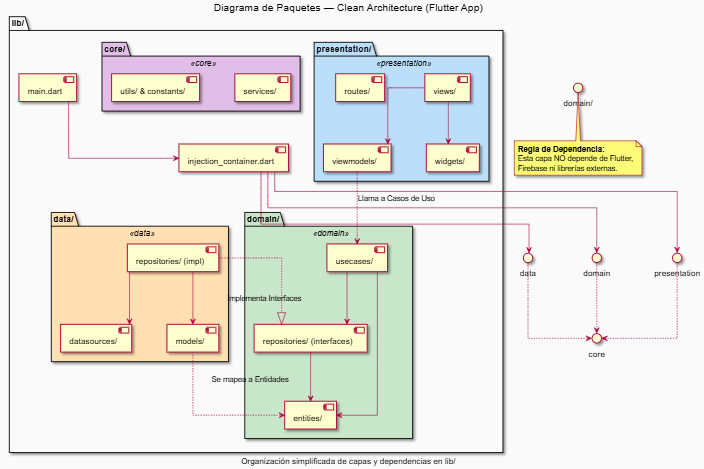
\includegraphics[width=0.8\textwidth]{img/arquitectura_clean.png}
  \caption{Flujo de datos bidireccional desde la capa de Presentación hasta el Origen de Datos mediado por los Casos de Uso.}
\end{figure}

\subsection{Diagrama de Despliegue}
Para comprender cómo interactúan físicamente los componentes de software desarrollados, se modeló la distribución de los nodos del sistema. Este diagrama evidencia la separación entre el dispositivo móvil (Turista), el navegador web (Propietario) y la infraestructura en la nube (Firebase).

\begin{figure}[H]
  \centering
  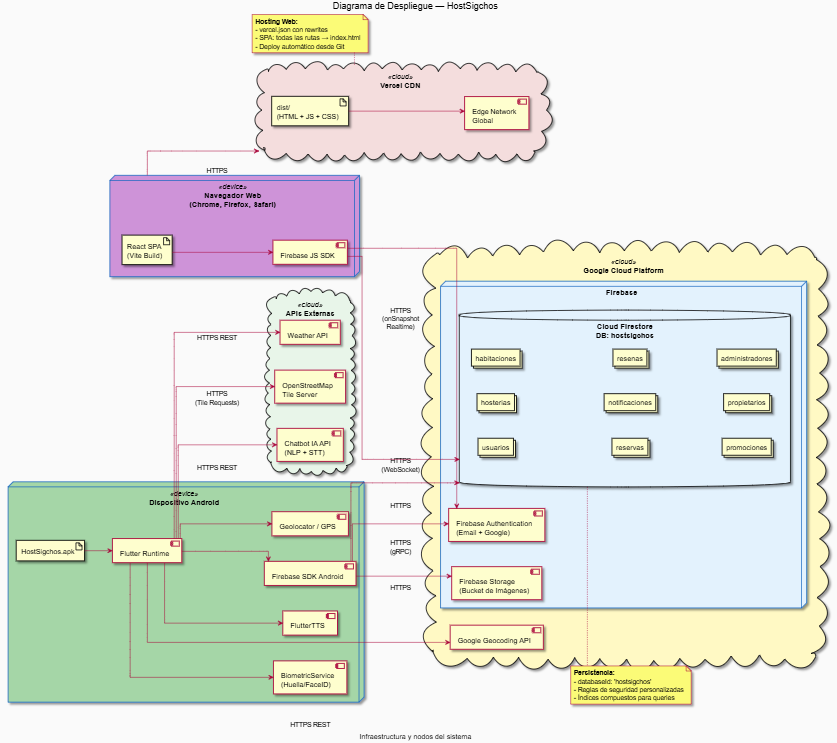
\includegraphics[width=0.8\textwidth]{img/uml_despliegue.png}
  \caption{Diagrama de Despliegue mostrando la topología física y los protocolos de comunicación.}
\end{figure}

\section{Stack Tecnológico, Herramientas y APIs Integradas}
Para construir un ecosistema altamente escalable e interactivo, HostSigchos se apoyó en un robusto abanico de tecnologías, librerías y APIs de terceros:

\begin{itemize}[label=$\blacksquare$]
    \item \textbf{Frameworks y Lenguajes:} \tech{Flutter} con el lenguaje \tech{Dart} para la aplicación móvil multiplataforma, y \tech{React JS} estilizado con \tech{Tailwind CSS} para el panel administrativo web.
    \item \textbf{Backend-as-a-Service (BaaS):} La infraestructura entera descansa sobre \tech{Google Firebase}. Se utilizan los módulos de \tech{Firebase Authentication} (OAuth 2.0 y Correo), \tech{Cloud Firestore} (Base de datos NoSQL en tiempo real mediante WebSockets), \tech{Firebase Storage} (Almacenamiento de imágenes de hosterías y perfiles) y \tech{Firebase Hosting} (Para desplegar los documentos legales estáticos).
    \item \textbf{APIs de Inteligencia Artificial y Datos:} Integración asíncrona (RESTful) con la \tech{Gemini API} (Google) para dotar de razonamiento al chatbot turístico, y \tech{OpenWeatherMap API} para consultas climatológicas en tiempo real de la zona de Sigchos.
    \item \textbf{Librerías de Hardware Nativo:} 
        \begin{itemize}
            \item \tech{local\_auth}: Para vincular el \textit{Secure Enclave} y habilitar autenticación con huella dactilar o FaceID.
            \item \tech{geolocator} y \tech{flutter\_compass}: Para acceder a la antena GPS y al magnetómetro (brújula) del celular.
            \item \tech{flutter\_tts} y \tech{speech\_to\_text}: Para proveer síntesis y reconocimiento de voz bidireccional en el chatbot.
        \end{itemize}
    \item \textbf{Servicios Cartográficos:} Se integró el motor \tech{flutter\_map} (basado en \textit{Leaflet}) consumiendo la capa de mapas de código abierto \tech{OpenStreetMap}.
    \item \textbf{Herramientas de Arquitectura:} \tech{Provider} como gestor de estado reactivo, \tech{GetIt} para la inyección de dependencias, y el paquete \tech{shimmer} para la ergonomía visual durante tiempos de carga por red (\textit{latencia}).
    \item \textbf{Asistencia de Desarrollo (Ingeniería de Software):} Se empleó la plataforma \tech{Google Antigravity} (IA Agentiva) para estandarizar la base de código y asegurar el cumplimiento de principios SOLID durante la estructuración de la Arquitectura Limpia, y el empaquetador \tech{MiKTeX} para compilar el presente documento LaTeX.
\end{itemize}

\section{Diagrama de carpetas}
La estructura física del proyecto móvil es un reflejo de la arquitectura descrita. La raíz `lib/` está compuesta por:

\begin{lstlisting}[style=codeblock]
HostSigchos/lib/
|-- core/                     # Elementos transversales al proyecto
|   |-- constants/            # Rutas de Firestore, variables ENV
|   |-- errors/               # Manejo global de excepciones (Failures)
|   |-- l10n/                 # Archivos de internacionalizacion
|   |-- services/             # Servicios de Hardware (Biometric, Notification)
|   +-- utils/                # Validadores, formateadores de fechas/precios
|
|-- data/                     # Capa de Acceso a Datos
|   |-- datasources/
|   |   |-- api/              # (Ej. openweathermap api)
|   |   |-- firebase/         # (Ej. auth_datasource.dart, reserva_datasource.dart)
|   |   +-- remote/           # (Ej. geocoding y chatbot Gemini api)
|   |-- models/               # Clases con fromJson/toJson
|   +-- repositories/         # Implementaciones concretas (...RepositoryImpl.dart)
|
|-- domain/                   # Capa de Dominio Pura (Dart Vainilla)
|   |-- entities/             # Entidades como Reserva, Habitacion, Hosteria
|   |-- repositories/         # Contratos/Interfaces abstractas
|   +-- usecases/             # Logica de negocio orquestada
|       |-- auth/
|       |-- habitacion/       # Ej: check_disponibilidad_usecase.dart
|       +-- reserva/          # Ej: crear_reserva_usecase.dart
|
|-- presentation/             # Capa Visual y Gestores de Estado
|   |-- routes/               # Tabla de enrutamiento (app_routes.dart)
|   |-- viewmodels/           # Gestores de estado (AuthViewModel, ReservaViewModel)
|   |-- views/                # Pantallas UI (19 pantallas en total)
|   |   |-- auth/
|   |   |-- chatbot/
|   |   |-- hosteria/
|   |   +-- reserva/
|   +-- widgets/              # Componentes UI reusables (Botones, Modales, Tarjetas)
|
|-- themes/                   # Definicion del ThemeData general (Colores, Tipografias)
|-- injection_container.dart  # Locator (GetIt) para inyeccion de dependencias
+-- main.dart                 # Inicializacion de Firebase, GetIt, Providers y RunApp
\end{lstlisting}

\section{Modelo de datos}
El backend principal se sostiene en \textbf{Cloud Firestore}. A pesar de ser una base de datos NoSQL documental, se modeló cuidadosamente simulando claves foráneas (como \pathtext{hosteriaId} o \pathtext{usuarioId}) que permiten realizar consultas robustas.

\begin{figure}[H]
  \centering
  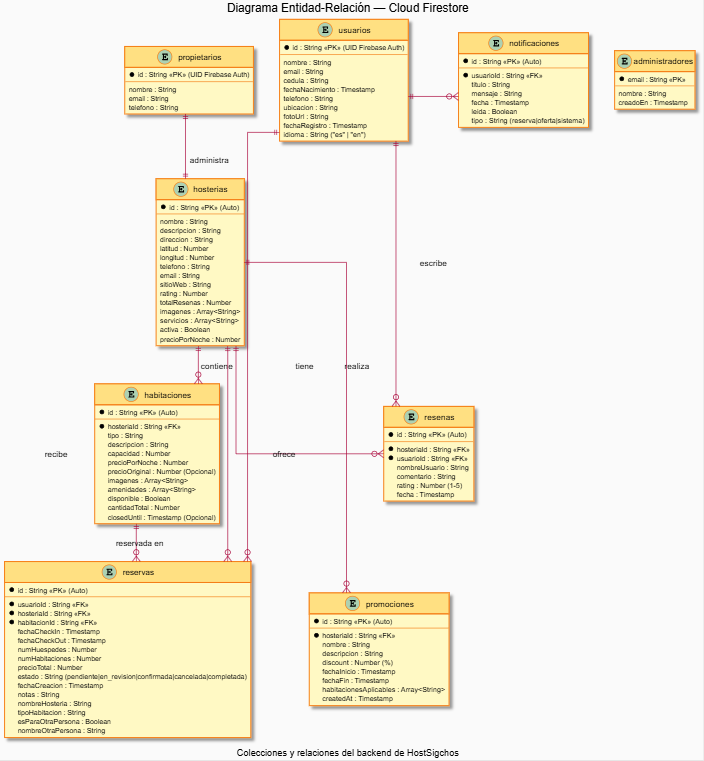
\includegraphics[width=0.8\textwidth]{img/modelo_firestore.png}
  \caption{Estructura documental y referencias simuladas (Foreign Keys) en Cloud Firestore.}
\end{figure}

Las colecciones principales operativas son:
\begin{itemize}
    \item \textbf{\pathtext{usuarios}:} Almacena información del turista (cédula, correo, avatar vinculado a Firebase Storage) y el UID proporcionado por Firebase Auth.
    \item \textbf{\pathtext{hosterias}:} Almacena coordenadas geográficas, imágenes de carrusel, amenidades, calificación media (rating) y descripción.
    \item \textbf{\pathtext{habitaciones}:} Colección dependiente lógicamente de la hostería (relacionada vía \linebreak \pathtext{hosteriaId}). Contiene precio por noche, cantidad disponible, capacidad y tipo de cama.
    \item \textbf{\pathtext{reservas}:} Documento transaccional central que guarda los detalles temporales (Check-in, Check-out), montos financieros (\pathtext{precioTotal}) y el \pathtext{estado} (Pendiente, Confirmada, Cancelada, Completada).
\end{itemize}

\section{Diagramas UML del Sistema}
Para proporcionar una vista integral de la ingeniería de software, se extrajeron los siguientes modelos unificados del proyecto, que abarcan la estructura estática, el comportamiento dinámico y la arquitectura:

\subsection{Diagrama de Componentes (Clean Architecture)}
Muestra la división macroscópica de los grandes bloques de software en capas de Dominio, Datos y Presentación, demostrando la alta cohesión y el bajo acoplamiento del código fuente.

\begin{figure}[H]
  \centering
  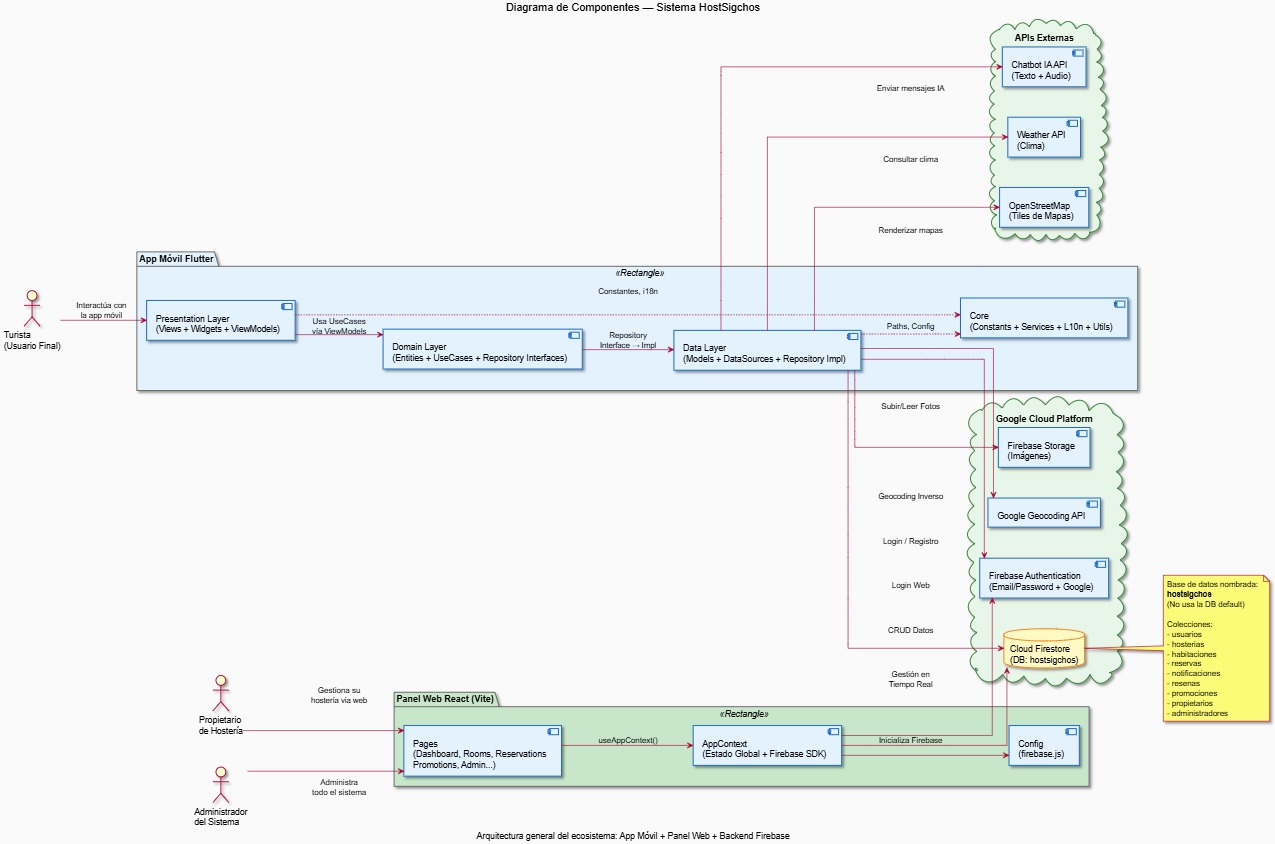
\includegraphics[width=0.8\textwidth]{img/uml_componentes.png}
  \caption{Diagrama de Componentes de la Arquitectura.}
\end{figure}

\subsection{Diagrama de Clases del Dominio}
Este diagrama ilustra la estructura estática de las Entidades Vainilla (Usuario, Reserva, Hostería, Habitación) y las relaciones semánticas entre ellas, siendo el núcleo de la aplicación, libre de dependencias de bases de datos externas.

\begin{figure}[H]
  \centering
  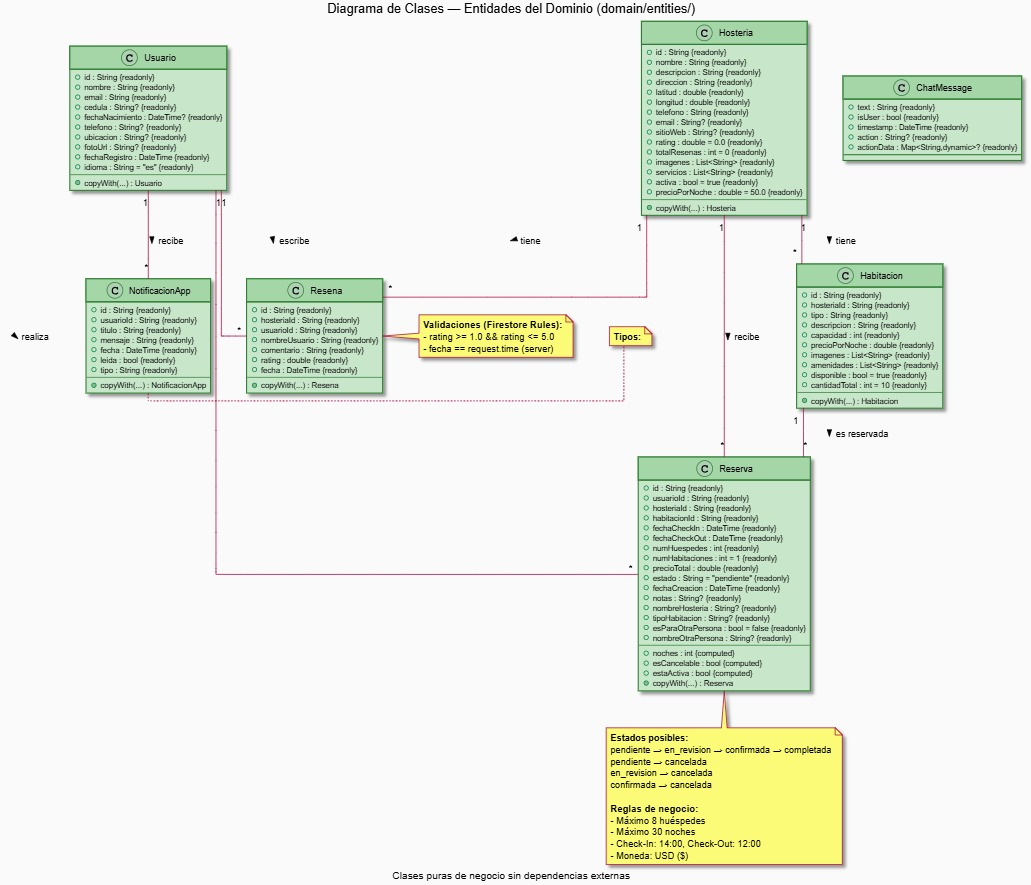
\includegraphics[width=0.8\textwidth]{img/uml_clases.png}
  \caption{Diagrama de Clases de las Entidades de Dominio.}
\end{figure}

\subsection{Diagrama de Casos de Uso}
Muestra la interacción fundamental entre los Turistas (Usuarios Móviles) y los Propietarios (Administradores) con los módulos principales del ecosistema, como exploración de hosterías, uso de IA, reservas y gestión de inventario.

\begin{figure}[H]
  \centering
  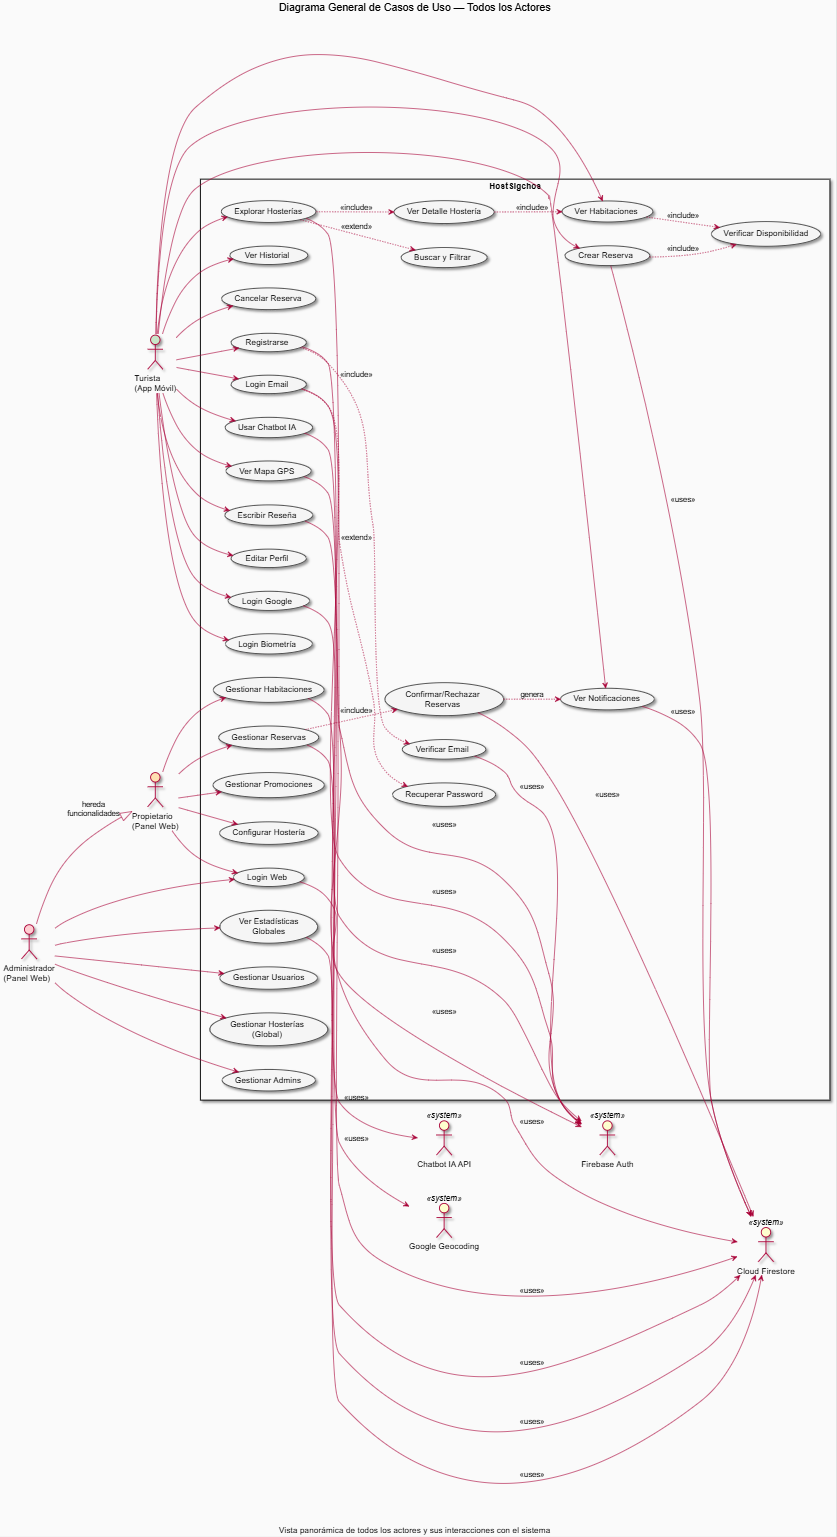
\includegraphics[width=0.7\textwidth]{img/uml_casos_uso.png}
  \caption{Diagrama de Casos de Uso general del sistema HostSigchos.}
\end{figure}

\subsection{Diagrama de Secuencia (o Actividad)}
Detalla el flujo lógico de comunicación transaccional entre el Cliente (Móvil), el Controlador de lógica (UseCase) y la Base de Datos (Firestore) para prevenir el cruce de fechas.

\begin{figure}[H]
  \centering
  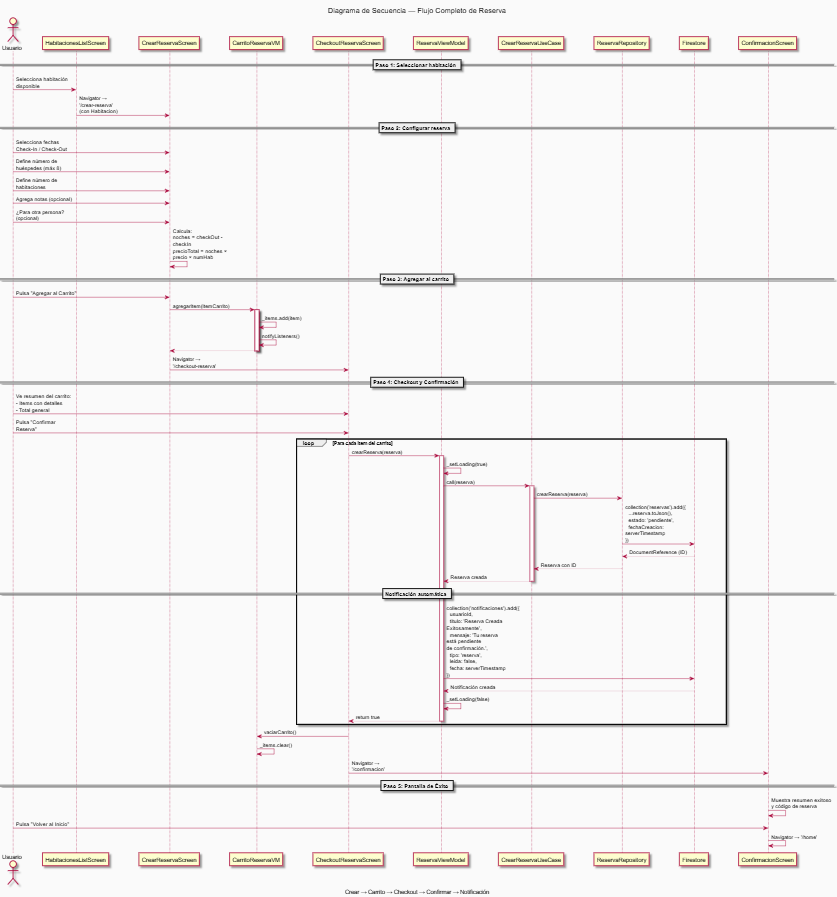
\includegraphics[width=0.8\textwidth]{img/uml_secuencia.png}
  \caption{Diagrama UML del flujo de reservas y validación.}
\end{figure}

\subsection{Máquina de Estados de Reserva}
Demuestra el ciclo de vida estricto de un documento de reserva dentro del ecosistema, mutando su estado asíncronamente (Pendiente, Confirmada, Cancelada, Completada) según la interacción del Administrador.

\begin{figure}[H]
  \centering
  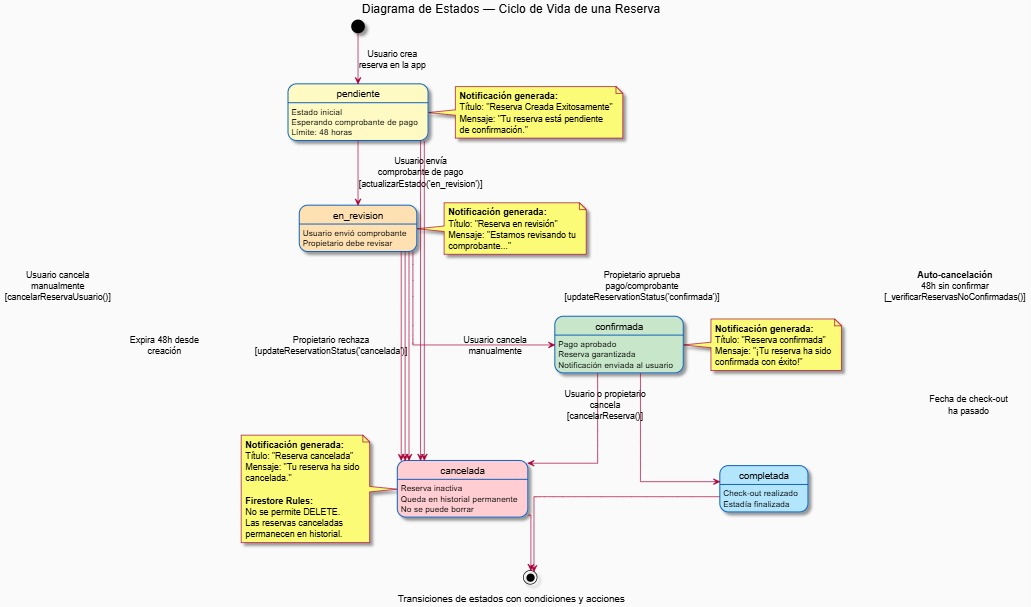
\includegraphics[width=0.8\textwidth]{img/uml_estados.png}
  \caption{Diagrama de Estados para el ciclo de vida transaccional.}
\end{figure}

\subsection{Diagrama Entidad-Relación Extendido (ER)}
A pesar de que Firebase Firestore es una base de datos documental (NoSQL), HostSigchos maneja dependencias lógicas fuertes. Este diagrama refleja cómo se conectan los documentos mediante referencias (Ej: \pathtext{hosteriaId}), simulando claves foráneas convencionales.

\begin{figure}[H]
  \centering
  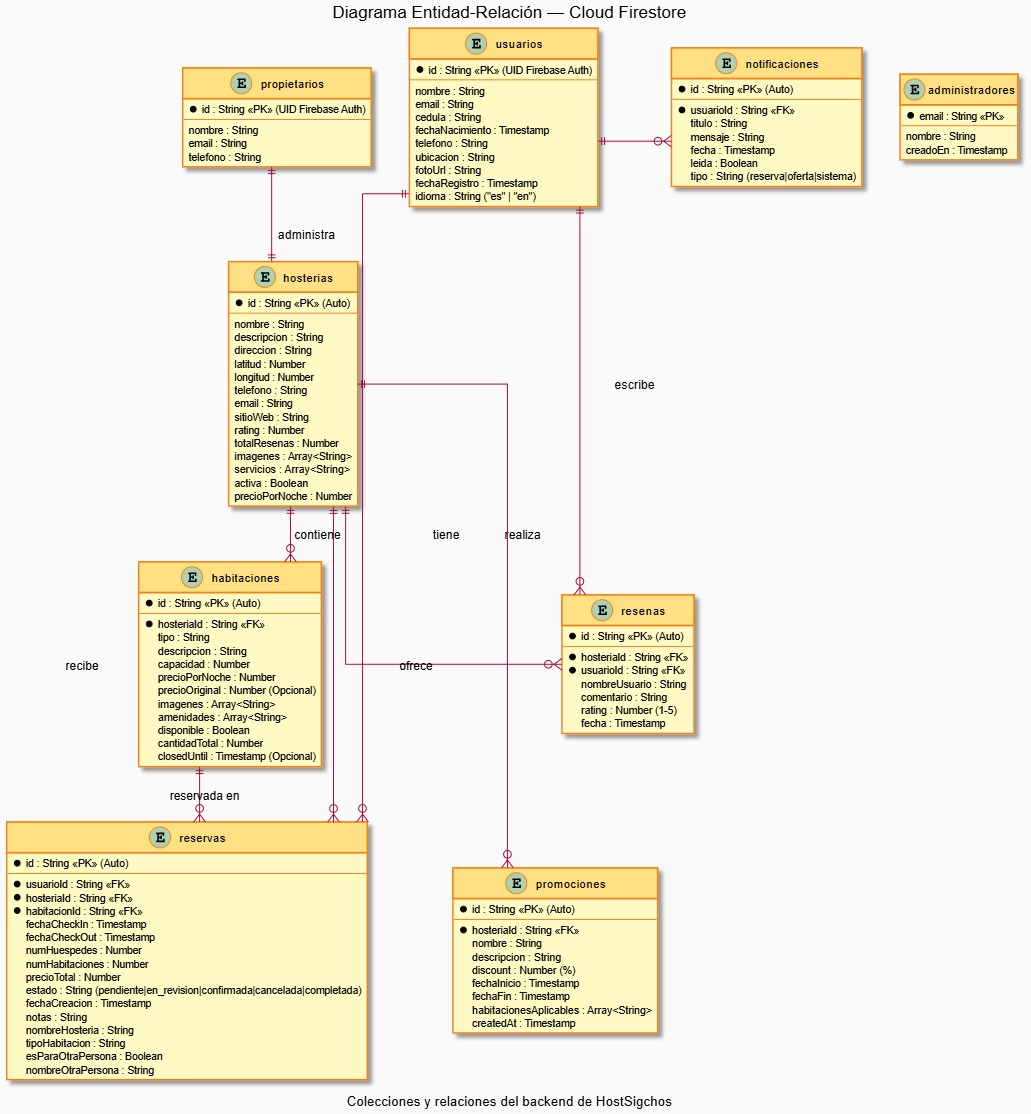
\includegraphics[width=0.8\textwidth]{img/uml_er.png}
  \caption{Diagrama ER lógico de las colecciones de Firestore.}
\end{figure}

\chapter{Desarrollo y capturas del aplicativo}

El sistema abarca diversas funcionalidades complejas que requieren sincronización asíncrona y uso intensivo del hardware del dispositivo móvil. Durante el ciclo de vida del proyecto, se estandarizó la base de código empleando arquitecturas limpias asistidas por \textbf{Antigravity}, una IA agentiva que aseguró el cumplimiento de principios SOLID. 
Se desarrollaron en total 19 rutas de pantalla (incluyendo interfaces móviles y web) completamente funcionales y validadas, orquestadas mediante 11 ViewModels (Provider) y 7 entidades de negocio. Adicionalmente, se integró una política incipiente de caché offline para mitigar pérdidas de conexión en zonas geográficas apartadas. A continuación se detalla con precisión milimétrica el desarrollo de todos los módulos.


\section{Módulo Web y Entorno Legal}
Previo al uso de la plataforma, los usuarios y propietarios interactúan con el portal web institucional. Este módulo aloja la \textbf{Landing Page} promocional, la cual explica las virtudes del sistema y fomenta la descarga del aplicativo móvil. Además, desde esta pantalla inicial, el usuario tiene la capacidad de cambiar el idioma de toda la plataforma gracias a un selector de internacionalización (\texttt{l10n}), garantizando accesibilidad inmediata para turistas extranjeros.
Asimismo, debido a las normativas estrictas de las tiendas de aplicaciones (Play Store y App Store), se redactaron e inyectaron las normativas legales mediante páginas web estáticas alojadas en Firebase Hosting.

\begin{figure}[H]
  \centering
  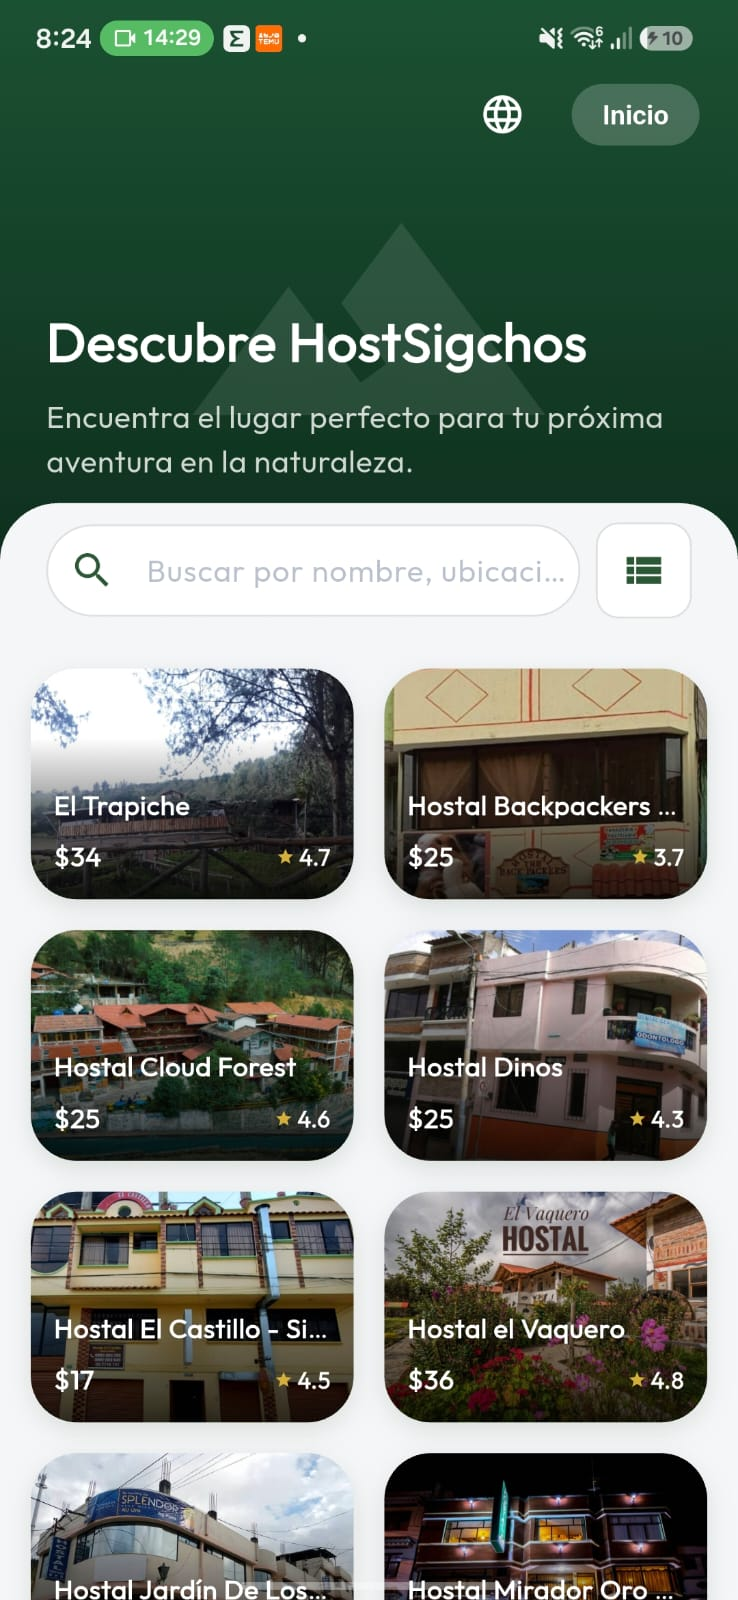
\includegraphics[width=0.45\textwidth]{img/landing_page.png}
  \caption{Landing Page promocional del ecosistema HostSigchos.}
\end{figure}

El usuario puede revisar las políticas y términos en cualquier momento, tanto desde la web como desde la aplicación móvil.
\begin{itemize}
    \item \textbf{Políticas de Privacidad:} \url{https://hostsigchos.web.app/politicas.html}
    \item \textbf{Términos y Condiciones:} \url{https://hostsigchos.web.app/terminos.html}
\end{itemize}

\begin{figure}[H]
  \centering
  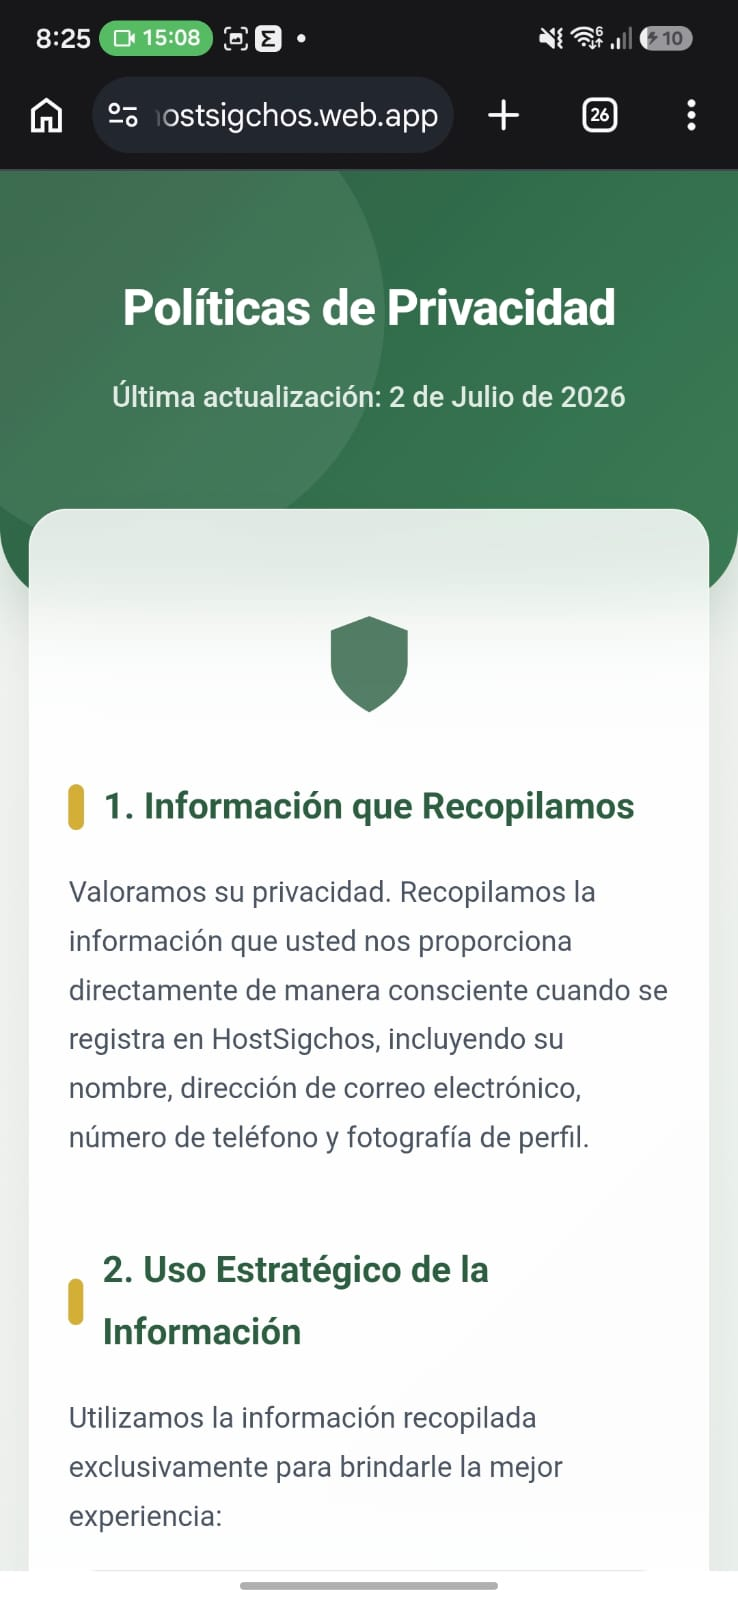
\includegraphics[width=0.45\textwidth]{img/politicas_privacidad.png}
  \caption{Visualización de las Políticas de Privacidad.}
\end{figure}

\begin{figure}[H]
  \centering
  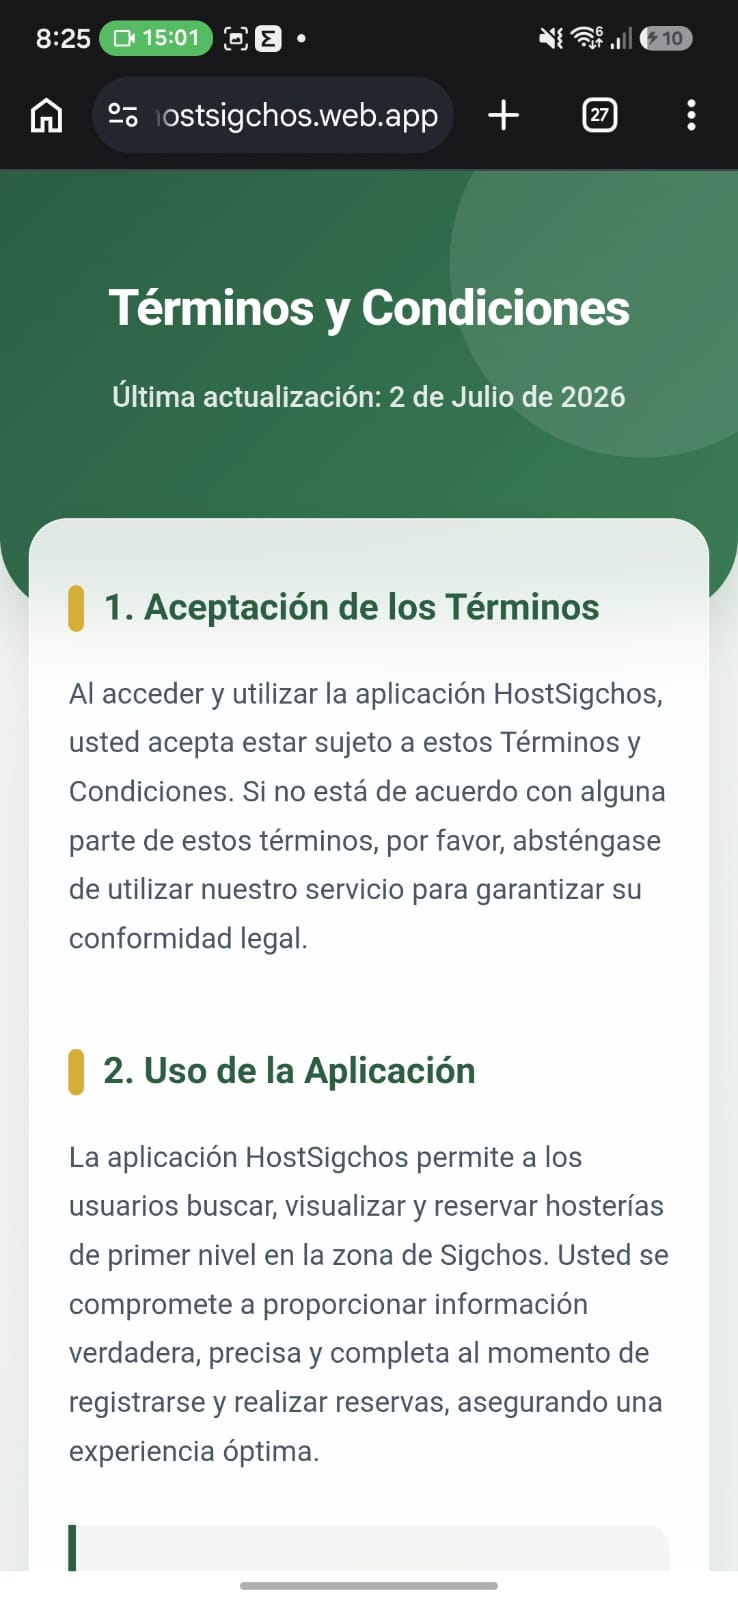
\includegraphics[width=0.45\textwidth]{img/terminos_condiciones.png}
  \caption{Documento legal de Términos y Condiciones.}
\end{figure}

\section{Módulo de Autenticación, Registro y Biometría}
El sistema de seguridad está diseñado para proteger los datos del turista y facilitar el acceso. El flujo principal comienza con la creación de una cuenta en Firebase Auth. El usuario puede ingresar mediante correo electrónico y contraseña o mediante un proveedor de OAuth 2.0 (Google Sign-In). 
Desde el punto de vista del desarrollo, el \pathtext{AuthViewModel} maneja los estados de \textit{cargando} (mostrando indicadores de progreso circular) y captura excepciones como contraseñas débiles o correos ya registrados, devolviendo al usuario un \textit{SnackBar} amigable. 

\begin{figure}[H]
  \centering
  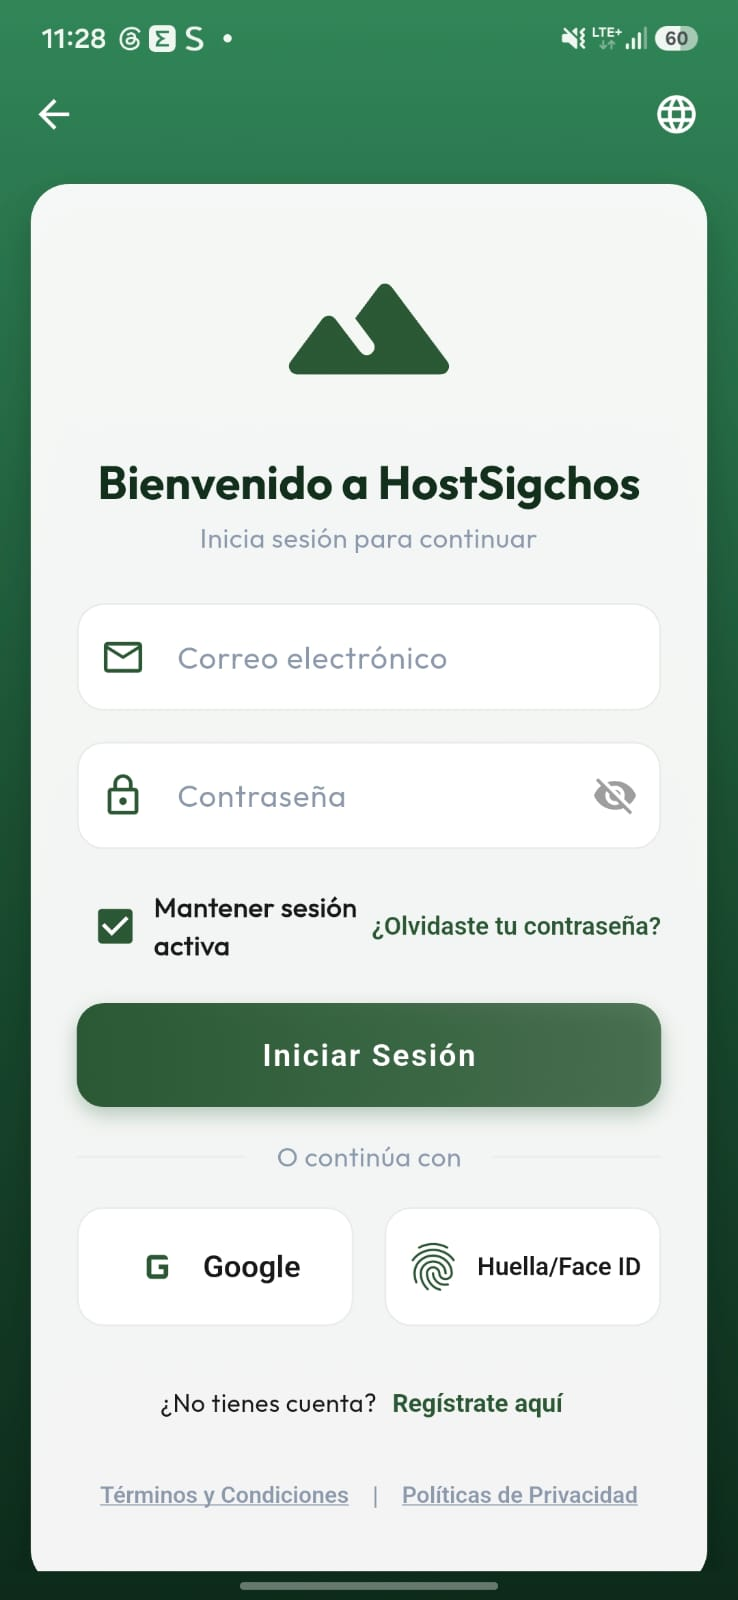
\includegraphics[width=0.45\textwidth]{img/login_screen.png}
  \caption{Pantalla de inicio de sesión clásica y SSO (Google).}
\end{figure}

\begin{figure}[H]
  \centering
  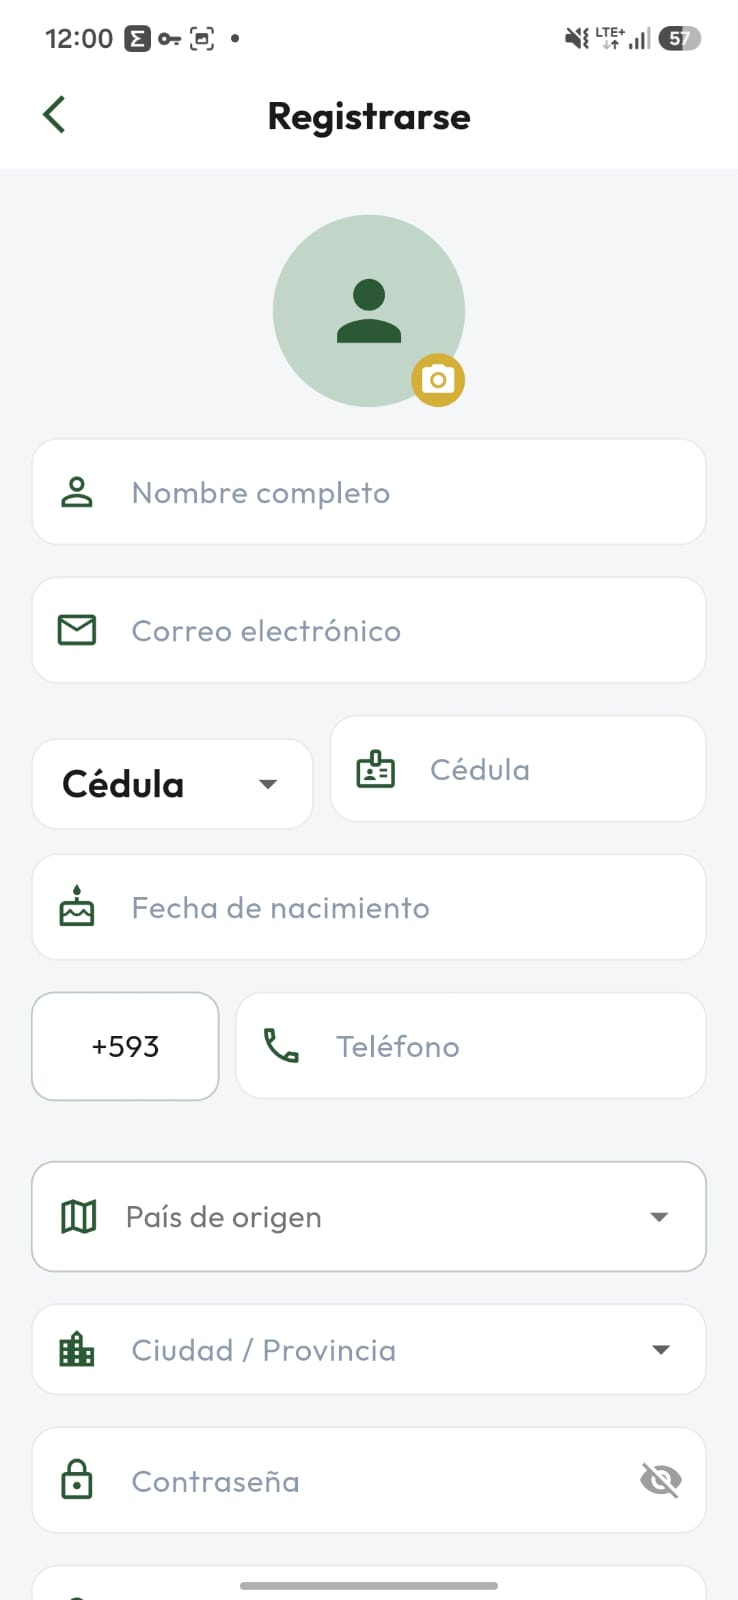
\includegraphics[width=0.45\textwidth]{img/registro_screen.png}
  \caption{Pantalla de registro con validaciones de formulario en tiempo real.}
\end{figure}

En caso de que el usuario pierda su acceso, se implementó un flujo de \textbf{Recuperación de Contraseña} mediante un enlace seguro enviado al correo del turista, posibilitando el auto-servicio en la gestión de credenciales.

\begin{figure}[H]
  \centering
  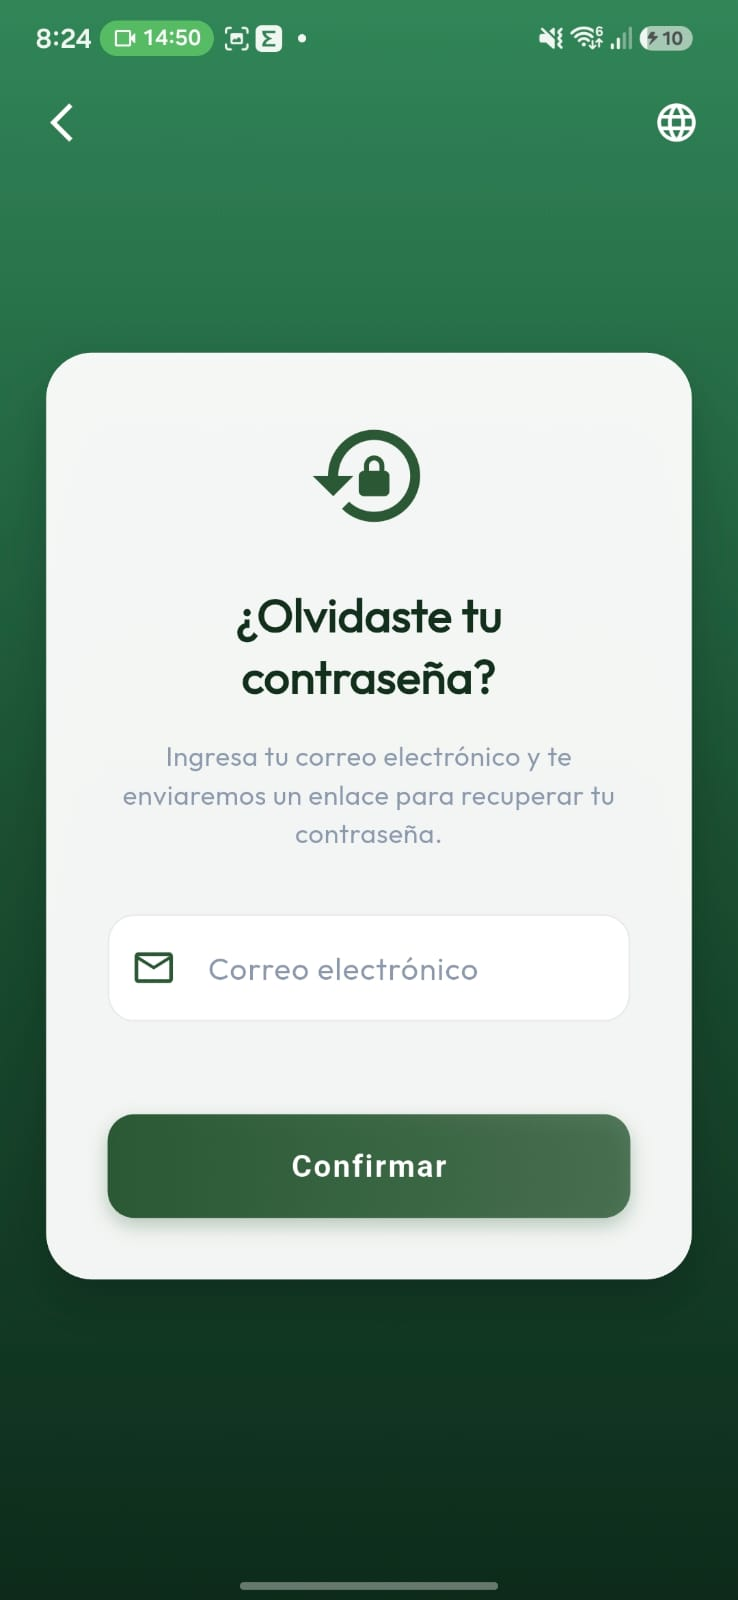
\includegraphics[width=0.45\textwidth]{img/forgot_password.png}
  \caption{Módulo de recuperación de contraseña vía correo electrónico.}
\end{figure}

Adicionalmente, desde la propia pantalla de Login, el usuario puede acceder al selector de idioma para adaptar la interfaz a su lengua materna de manera instantánea, sin necesidad de autenticarse previamente.

Para elevar el estándar de seguridad y mejorar la experiencia de usuario (UX), se integró la verificación biométrica del hardware (Huella Dactilar o Reconocimiento Facial) usando la librería \tech{local\_auth}. Esta validación se apoya en el \textit{Secure Enclave} del dispositivo para evitar robos de identidad \cite{firebaseDocs}.

\begin{lstlisting}[style=codeblock,caption={Lógica asíncrona de autenticación biométrica utilizando el hardware nativo.}]
// Función inyectada en el AuthViewModel
Future<bool> autenticarConBiometria() async {
  final LocalAuthentication auth = LocalAuthentication();
  bool canAuthenticateWithBiometrics = await auth.canCheckBiometrics;
  
  if (canAuthenticateWithBiometrics) {
    return await auth.authenticate(
      localizedReason: 'Por favor, autentícate para acceder a HostSigchos',
      options: const AuthenticationOptions(biometricOnly: true),
    );
  }
  return false; // Fallback a contraseña manual
}
\end{lstlisting}

\begin{figure}[H]
  \centering
  %\includegraphics[width=0.45\textwidth]{img/biometrica.png}
  \caption{Autenticación biométrica habilitada por el hardware nativo.}
\end{figure}

\section{Módulo de Exploración (Dashboard) y Visualización de Hosterías}
Una vez autenticado, el turista ingresa al \pathtext{Dashboard} principal. Esta pantalla consume el \pathtext{HosteriaViewModel}, recuperando la lista de hosterías desde Firestore. Para contrarrestar problemas de red (alta latencia) y evitar bloqueos en la UI, se implementó el paquete \tech{shimmer}, el cual renderiza un esqueleto gris animado mientras los datos terminan de descargar. 
El usuario tiene la opción de alternar la vista entre un layout de \textbf{Lista} y uno de \textbf{Cuadrícula}, maximizando la ergonomía visual. Las imágenes pesadas se cachean asíncronamente vía \tech{cached\_network\_image}.

\begin{figure}[H]
  \centering
  
\includegraphics[width=0.45\textwidth]{img/dashboard_lista.png}
  \caption{Dashboard principal de exploración en formato Lista.}
\end{figure}

\begin{figure}[H]
  \centering
  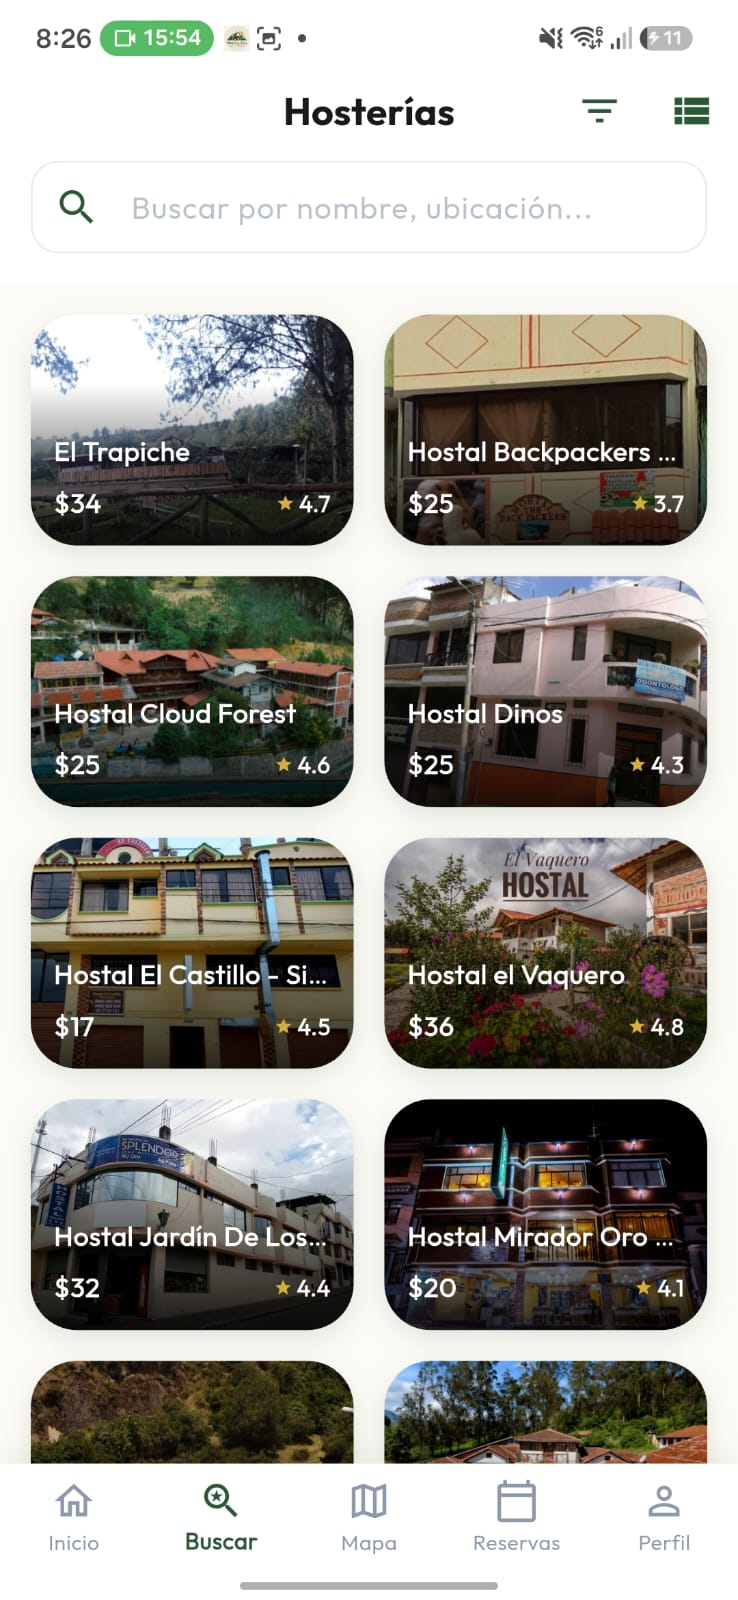
\includegraphics[width=0.45\textwidth]{img/dashboard_cuadricula.png}
  \caption{Dashboard principal de exploración alternado al formato Cuadrícula.}
\end{figure}

Al seleccionar una hostería, se navega al detalle de la misma. Aquí el usuario puede visualizar un carrusel dinámico de las instalaciones, chips de amenidades (Wi-Fi, piscina, etc.) y acceder al \textbf{Apartado de Reseñas} donde los huéspedes previos califican con estrellas su estadía, brindando retroalimentación comunitaria.

\begin{figure}[H]
  \centering
  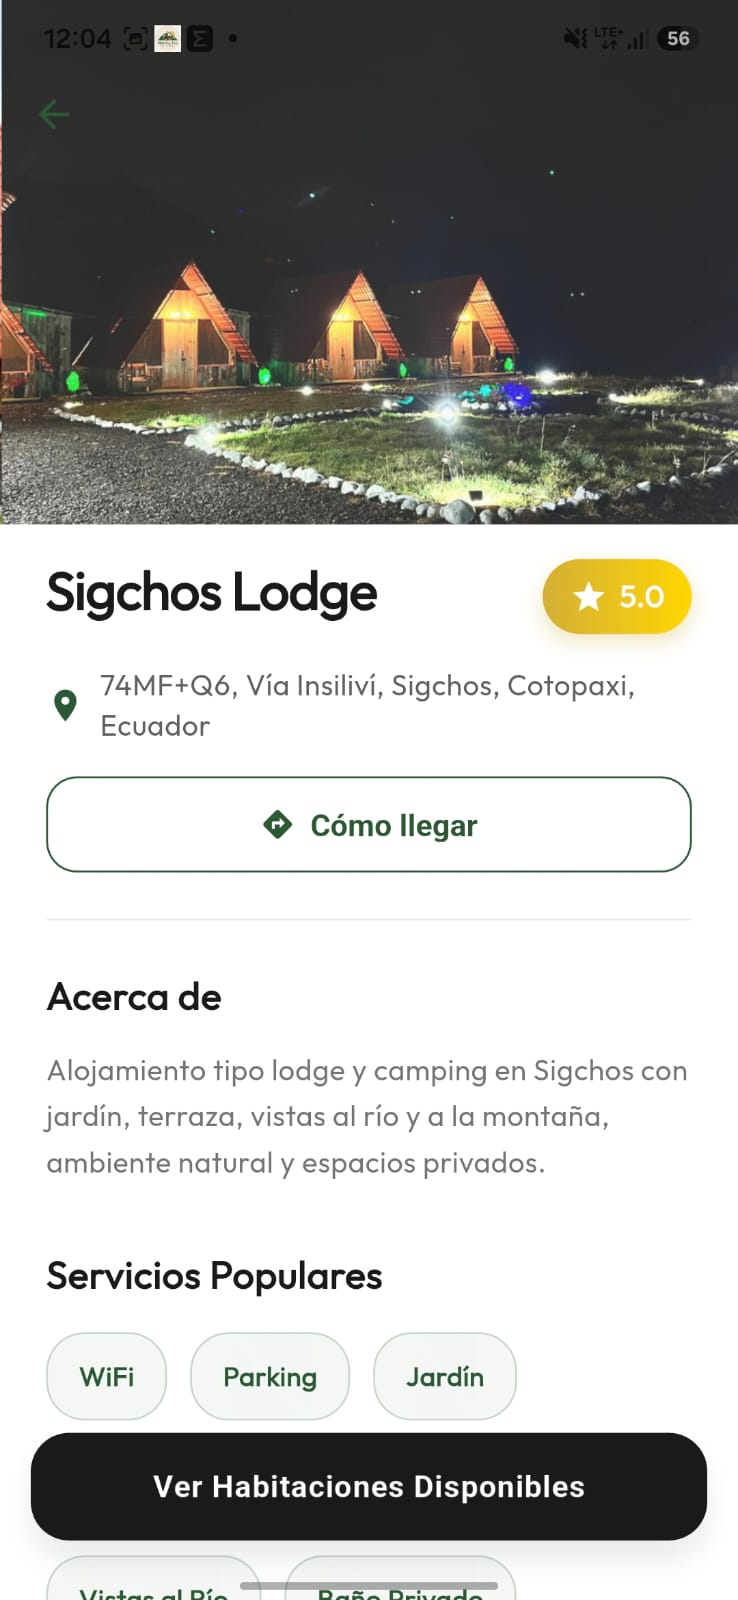
\includegraphics[width=0.45\textwidth]{img/detalle_hosteria_screen.png}
  \caption{Vista detallada de los servicios generales de una hostería.}
\end{figure}

\begin{figure}[H]
  \centering
  
\includegraphics[width=0.45\textwidth]{img/resenas.png}
  \caption{Módulo comunitario de calificación y reseñas.}
\end{figure}

Dentro del detalle, el turista puede acceder a la \textbf{Visualización de Habitaciones}, donde se despliegan las capacidades, tipos de cama y precios de cada alcoba disponible.

\begin{figure}[H]
  \centering
  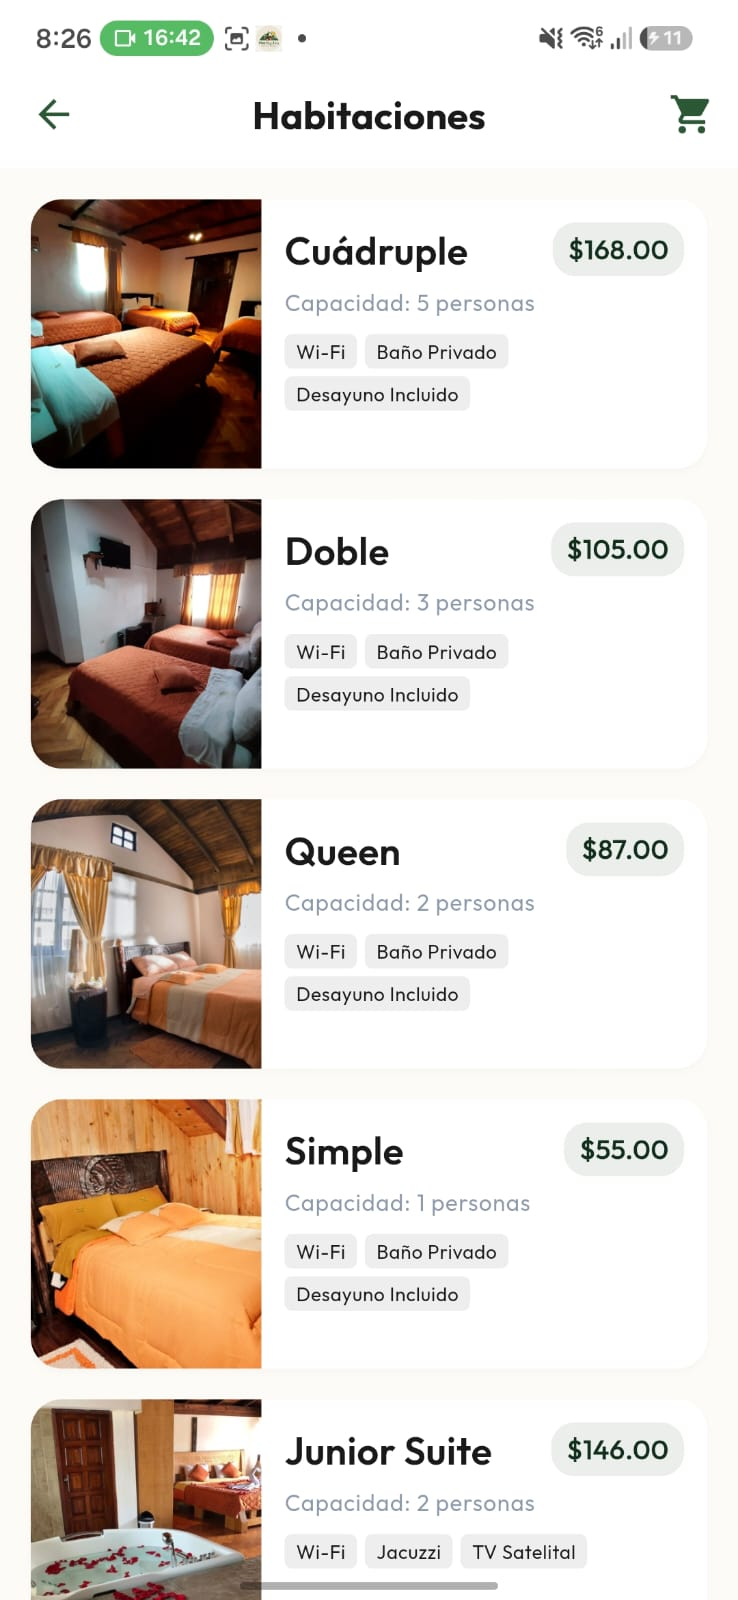
\includegraphics[width=0.45\textwidth]{img/habitaciones.png}
  \caption{Catálogo detallado de habitaciones y precios por noche.}
\end{figure}

\section{Módulo de Mapas Interactivos y Geolocalización}
El turismo requiere orientación espacial precisa. Se incorporó un módulo de mapas implementado con el paquete \tech{flutter\_map} (motor Leaflet) y las capas base de OpenStreetMap. 
A nivel de desarrollo, se utiliza el paquete \tech{geolocator} para solicitar permisos de GPS y obtener la latitud y longitud actual del usuario. Adicionalmente, se integró el paquete \tech{flutter\_compass} para hacer que el mapa rote según la orientación física del teléfono. Los \textit{Markers} (puntos de interés) se renderizan leyendo las coordenadas de las hosterías alojadas en la base de datos, lo que permite trazar rutas y distancias estimadas.

\begin{figure}[H]
  \centering
  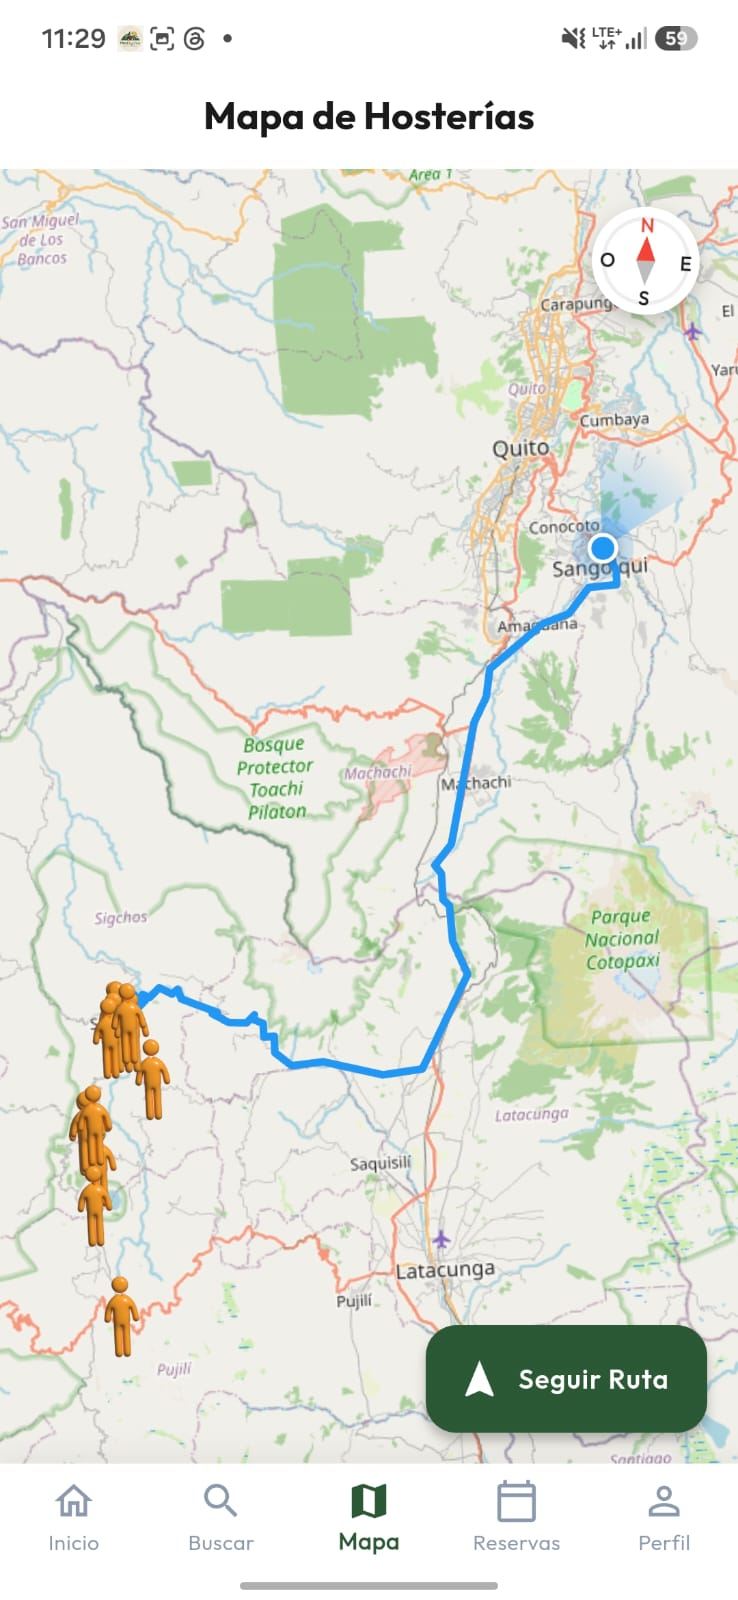
\includegraphics[width=0.45\textwidth]{img/mapa_screen.png}
  \caption{Pantalla de visualización de mapas integrando los marcadores de hosterías y geolocalización.}
\end{figure}

\section{Asistente Virtual (Chatbot con Inteligencia Artificial)}
Considerando la necesidad de guías turísticos 24/7, se construyó un Chatbot inteligente alimentado por la API de \tech{Gemini} (Google). 
El \pathtext{ChatbotViewModel} gestiona el historial de la conversación (prompts) en una lista local. El sistema inyecta un contexto inicial (\textit{System Instruction}) indicándole a la IA que asuma el rol de guía experto en Sigchos. 

Durante la fase de pruebas del sistema, se detectaron errores de saturación (Rate Limit \texttt{429}) al consumir la API gratuita de Gemini. Esto se solventó abstrayendo el manejo de error y devolviendo un estado controlado a la UI que invita al usuario a reintentar en lugar de colapsar la aplicación. Además, el módulo interactúa asíncronamente con la API de \tech{OpenWeatherMap} para brindar respuestas del clima en tiempo real, y utiliza los paquetes nativos de \tech{flutter\_tts} y \tech{speech\_to\_text} para interacción por voz.

\begin{figure}[H]
  \centering
  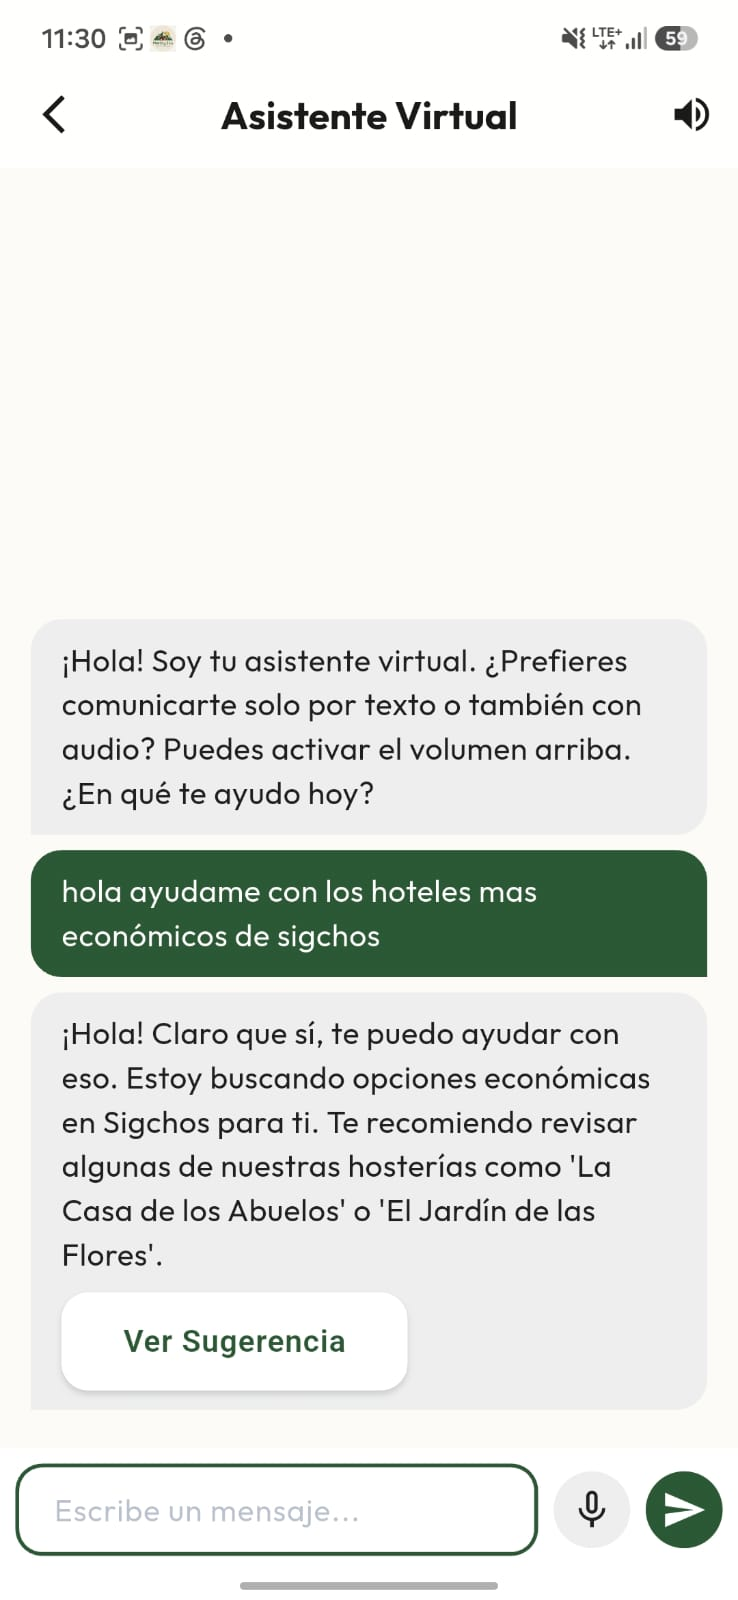
\includegraphics[width=0.45\textwidth]{img/chatbot_screen.png}
  \caption{Asistente turístico integrado, respondiendo con texto y voz.}
\end{figure}

\section{Proceso de Reserva y Resolución del Overbooking}
El flujo transaccional es el núcleo de HostSigchos. Una vez que el usuario selecciona una habitación ingresa al \textbf{Módulo de Reservas}, donde debe introducir su fecha de \textit{Check-in} y \textit{Check-out} a través de un selector de calendario (\tech{DateRangePickerDialog}).

\begin{figure}[H]
  \centering
  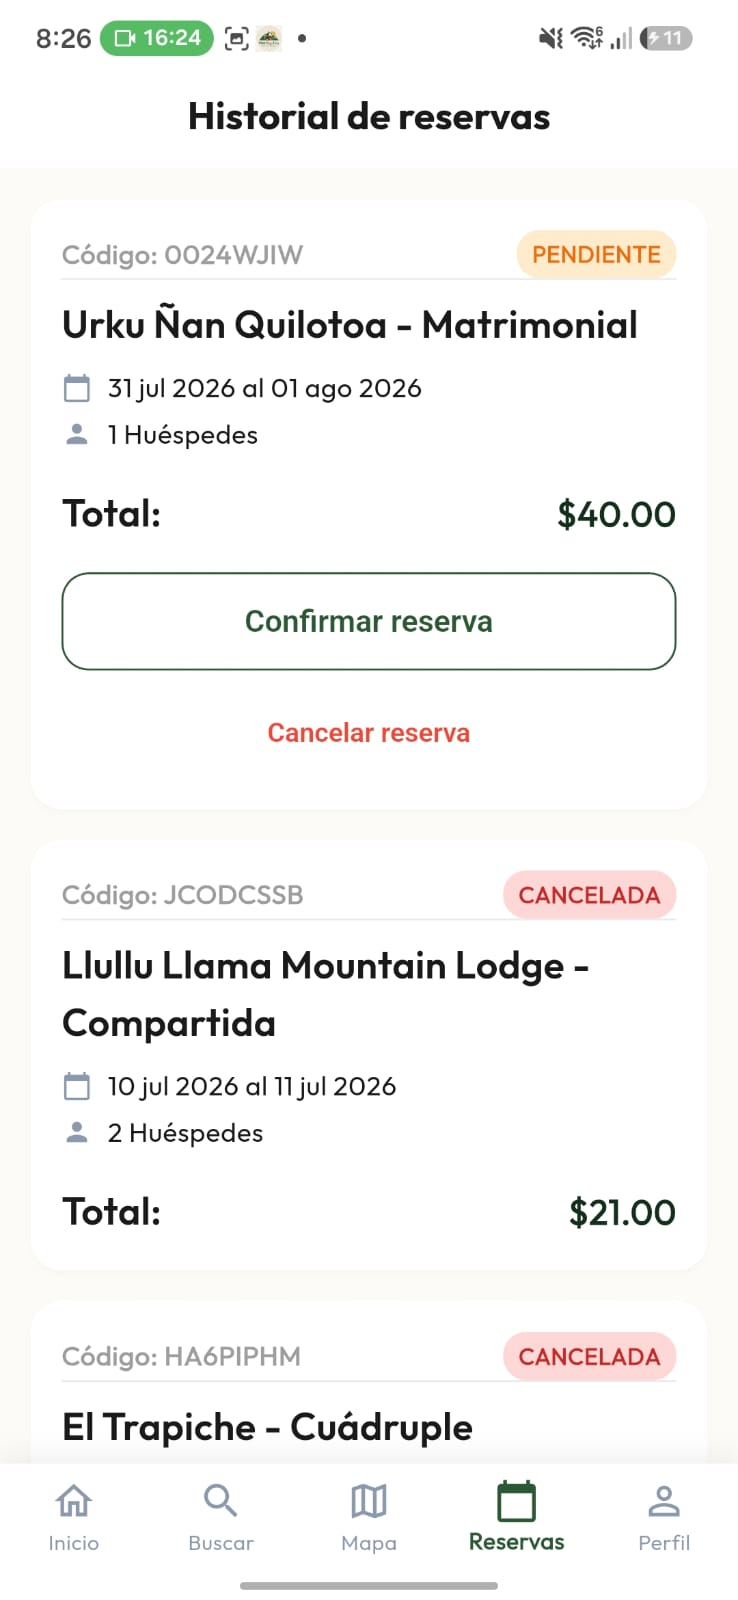
\includegraphics[width=0.45\textwidth]{img/modulo_reservas.png}
  \caption{Módulo centralizado de gestión y solicitud de nueva reserva.}
\end{figure}

Para prevenir el \textit{Overbooking} (sobreventa), el \pathtext{VerificarDisponibilidadUseCase} recupera todas las reservas con estado ``Pendiente'' o ``Confirmada'' para dicha habitación y ejecuta un motor matemático de colisiones temporales en milisegundos:

\begin{lstlisting}[style=codeblock,caption={Lógica pura en Dart para prevención de superposición temporal de fechas.}]
// Dentro de domain/usecases/habitacion/verificar_disponibilidad_usecase.dart
bool isDisponible = true;
int habitacionesOcupadas = 0;

for (var r in reservasExistentes) {
    // Si la nueva fecha de ingreso es ANTES de la salida existente
    // Y la nueva fecha de salida es DESPUES del ingreso existente, hay cruce.
    if (checkIn.isBefore(r.fechaCheckOut) && checkOut.isAfter(r.fechaCheckIn)) {
        habitacionesOcupadas += r.numHabitaciones;
    }
}
if(habitacionesOcupadas >= habitacion.cantidadTotal) {
    isDisponible = false; // Se bloquea la reserva
}
\end{lstlisting}

\begin{figure}[H]
  \centering
  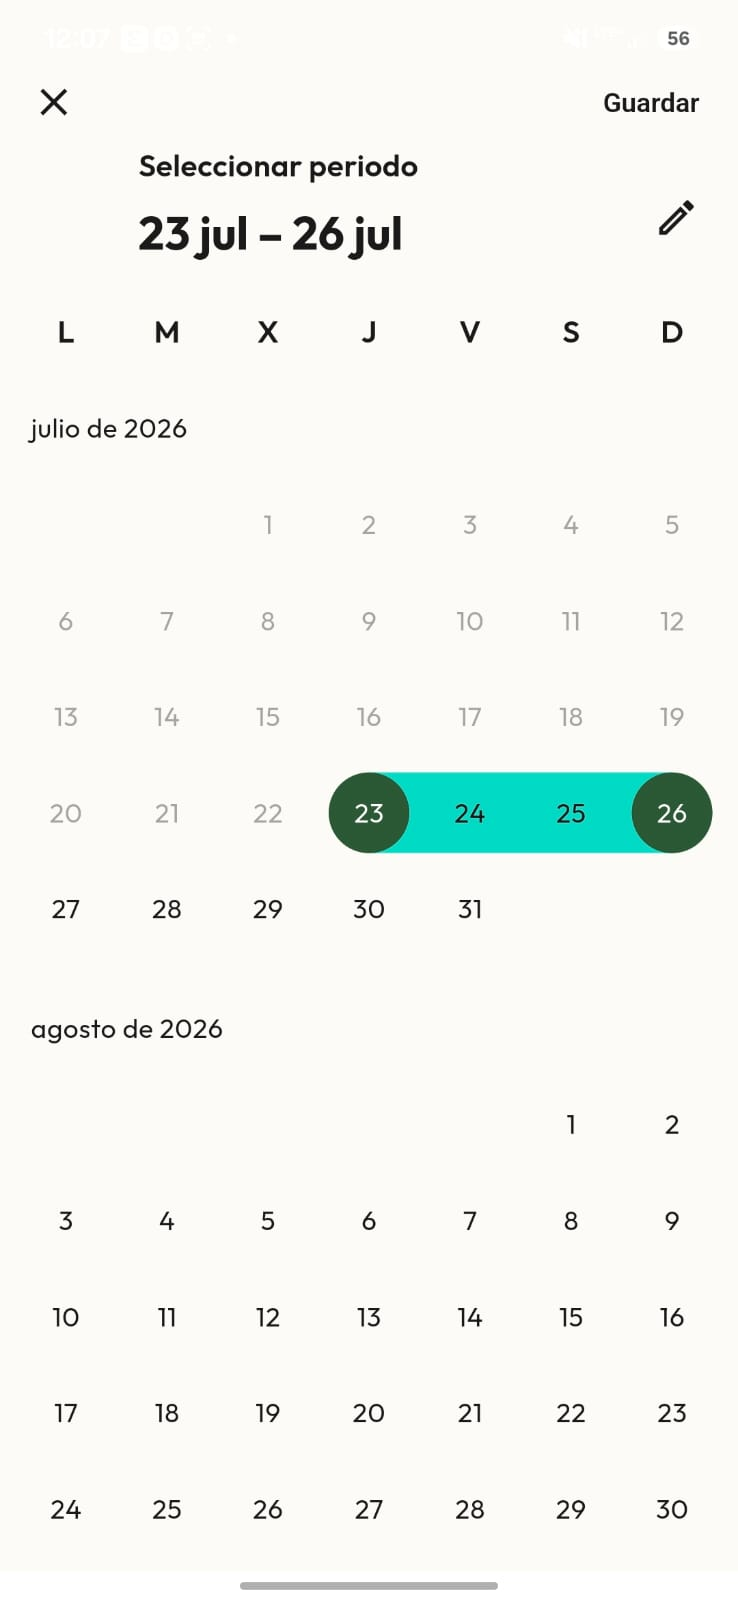
\includegraphics[width=0.45\textwidth]{img/seleccion_fechas_screen.png}
  \caption{Selector de rango de fechas para validación de disponibilidad.}
\end{figure}

\begin{figure}[H]
  \centering
  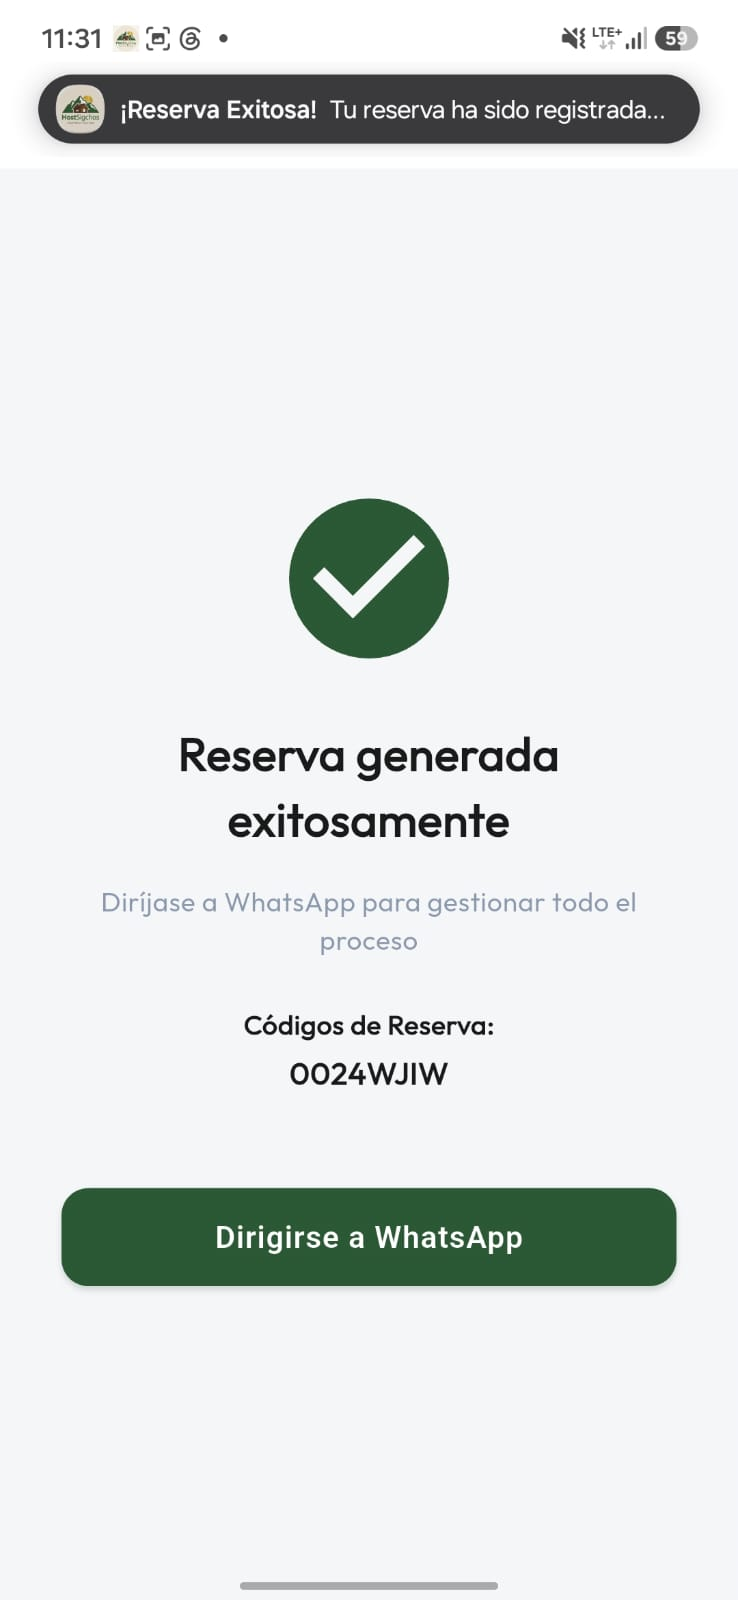
\includegraphics[width=0.45\textwidth]{img/checkout_screen.png}
  \caption{Proceso de \textit{Checkout} detallando costos antes del guardado final.}
\end{figure}

\section{Módulo de Usuario, Ajustes y Notificaciones}
El perfil del turista en HostSigchos es altamente personalizable. El usuario puede acceder a la sección de \textbf{Editar Perfil} para actualizar sus datos de contacto, contraseña y fotografía, la cual es cargada directamente a los buckets seguros de \tech{Firebase Storage}. Desde este mismo apartado, el usuario posee el control total para cambiar el \textbf{Idioma} de la aplicación, el cual es inyectado globalmente mediante un \pathtext{LocaleProvider}.

\begin{lstlisting}[style=codeblock,caption={Lógica del LocaleProvider para el cambio de idioma en tiempo real.}]
// provider/locale_provider.dart
class LocaleProvider extends ChangeNotifier {
  Locale _locale = const Locale('es'); // Español por defecto

  Locale get locale => _locale;

  void setLocale(Locale newLocale) {
    if (!L10n.all.contains(newLocale)) return;
    _locale = newLocale;
    notifyListeners(); // Re-renderiza toda la App reactivamente
  }
}
\end{lstlisting}

\begin{figure}[H]
  \centering
  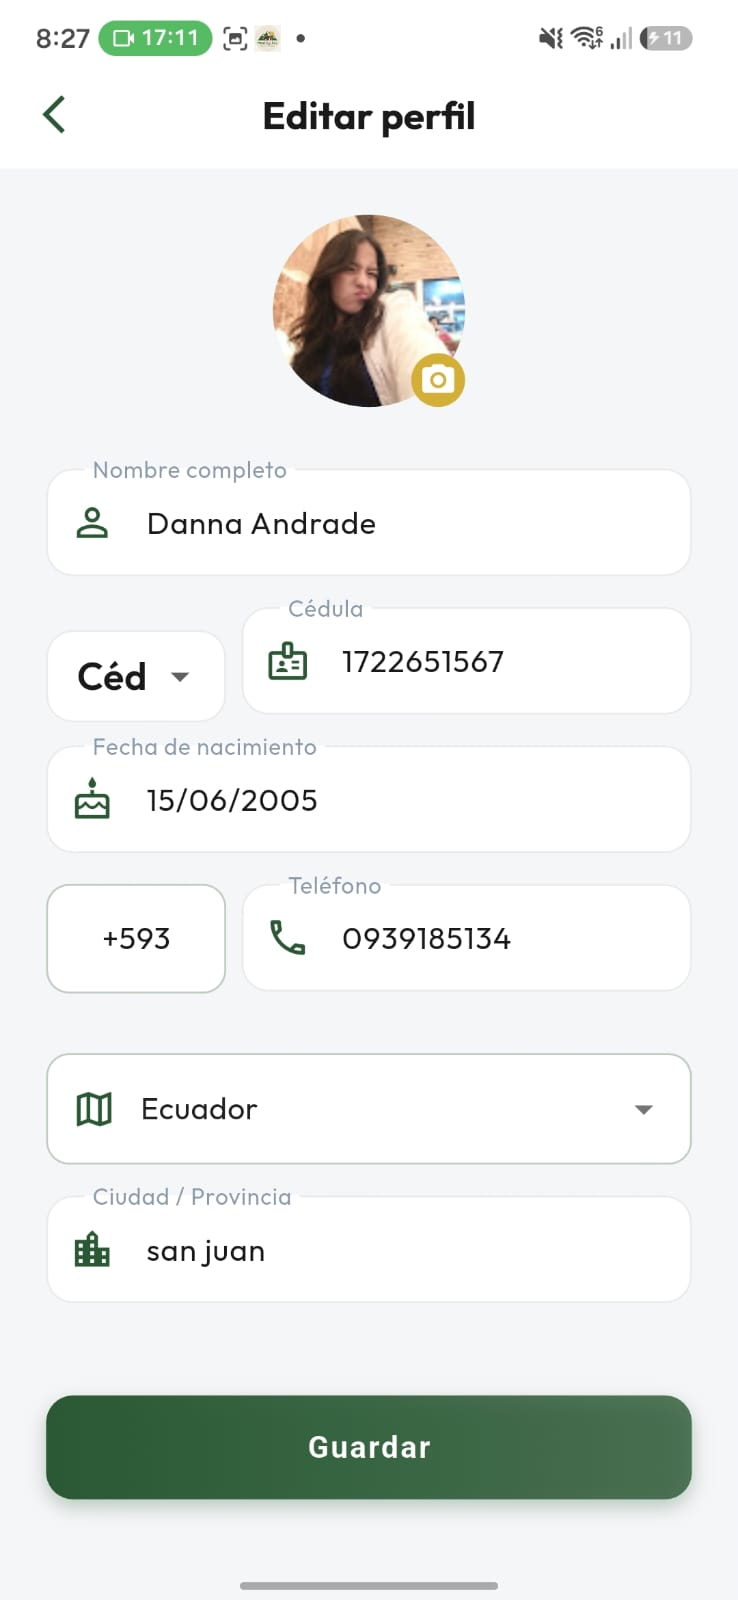
\includegraphics[width=0.45\textwidth]{img/editar_perfil.png}
  \caption{Interfaz de configuración y edición del perfil del turista.}
\end{figure}

Por mandato de las políticas de Google Play Store, se implementó de forma obligatoria el flujo de \textbf{Eliminar Cuenta}. El usuario puede desvincular sus datos permanentemente de los servidores mediante un botón en la app y una confirmación legal en la web a través del enlace: \url{https://hostsigchos.web.app/eliminar_cuenta.html}.

\begin{figure}[H]
  \centering
  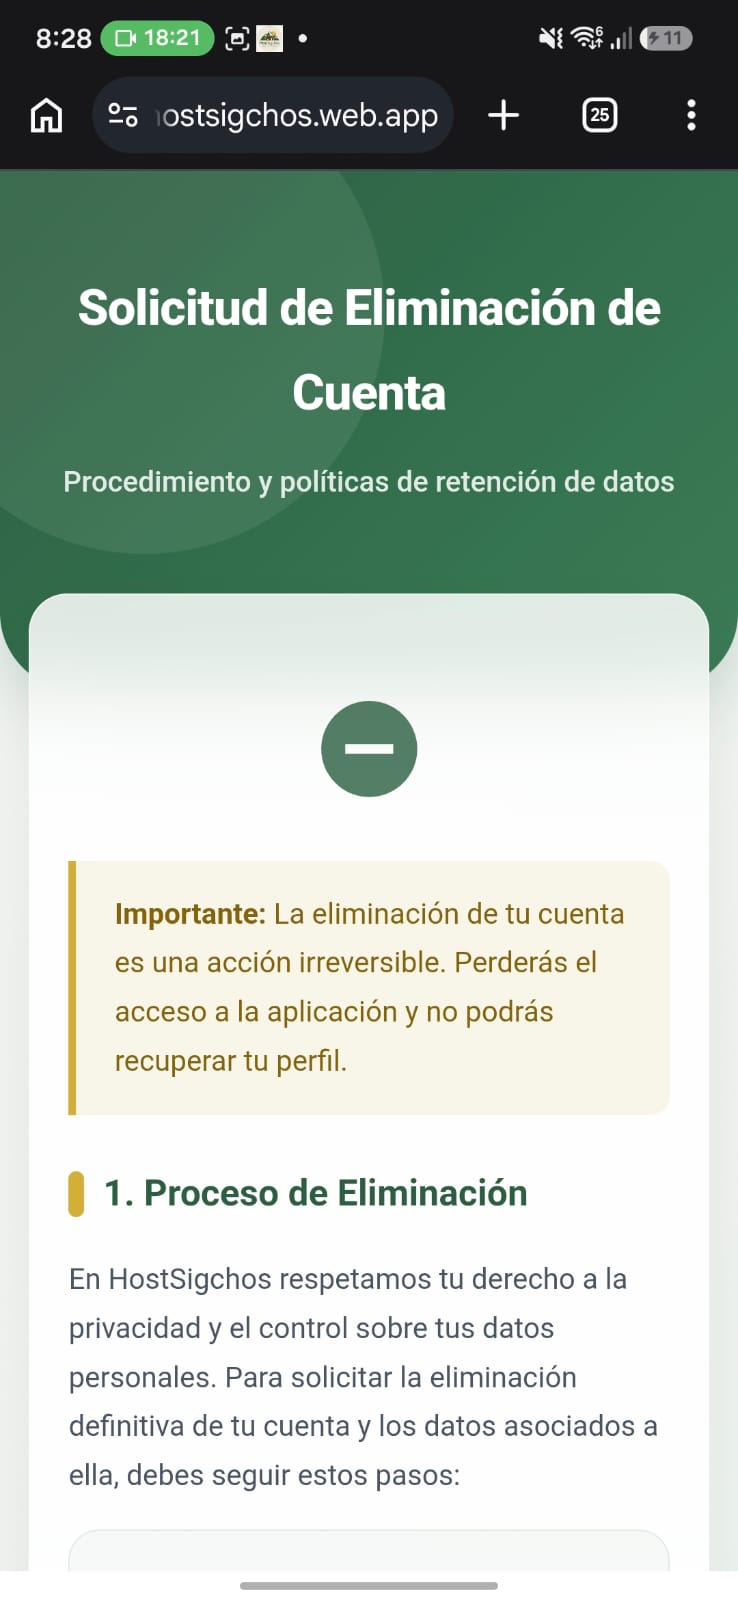
\includegraphics[width=0.45\textwidth]{img/eliminar_cuenta.png}
  \caption{Flujo de seguridad para la eliminación definitiva de la cuenta.}
\end{figure}

Además, el turista dispone de un canal dedicado de \textbf{Ayuda y Soporte} para resolver problemas con su cuenta, y un gestor de \textbf{Notificaciones Push} (vía \tech{flutter\_local\_notifications}) que le alertan cuando el administrador confirma o cancela su reserva, uniendo la experiencia del mundo offline con el mundo digital.

\begin{figure}[H]
  \centering
  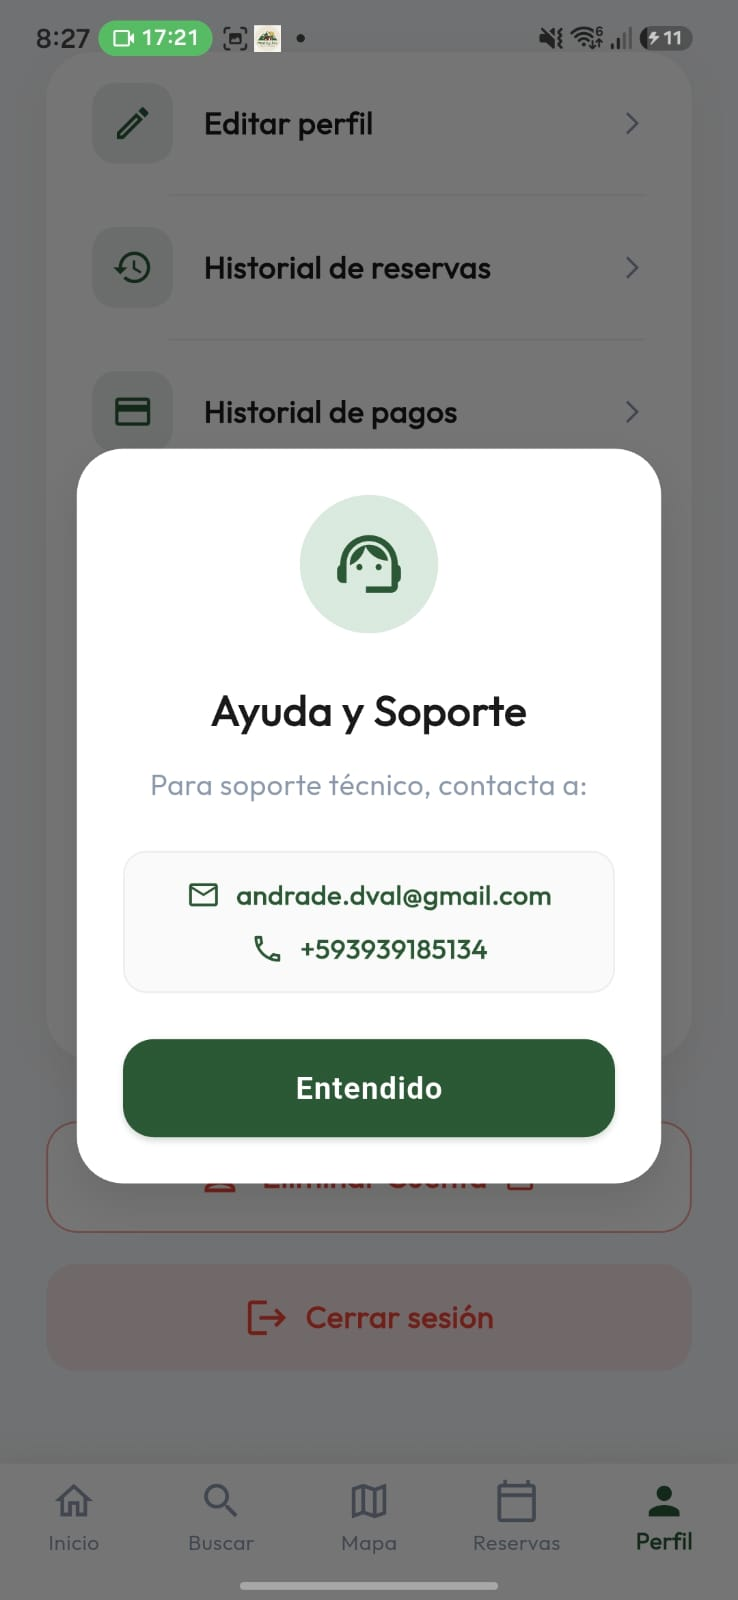
\includegraphics[width=0.45\textwidth]{img/ayuda_soporte.png}
  \caption{Centro de Ayuda y Soporte técnico al cliente.}
\end{figure}

\begin{figure}[H]
  \centering
  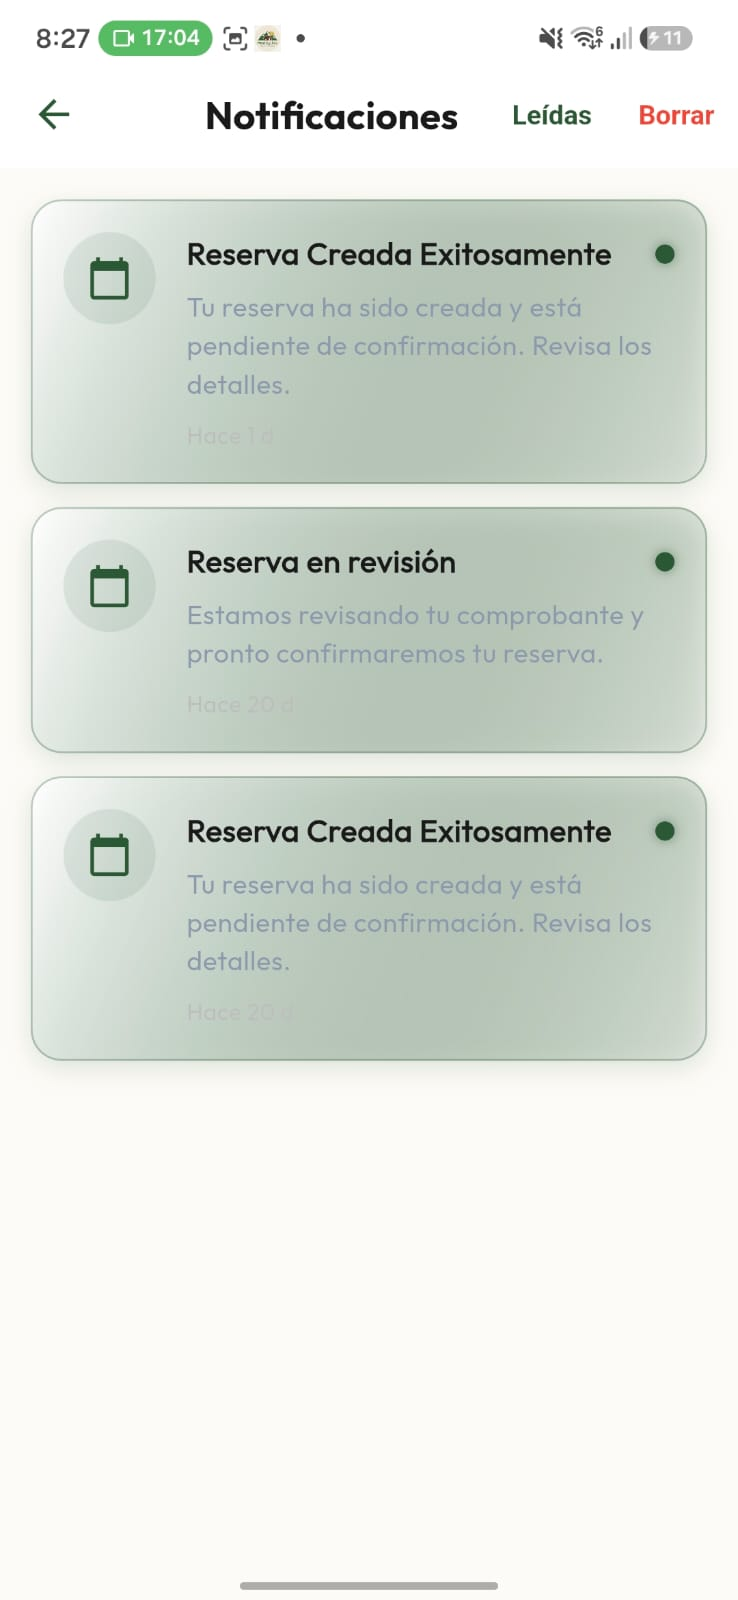
\includegraphics[width=0.45\textwidth]{img/notificaciones.png}
  \caption{Bandeja de entrada de Notificaciones Push sobre el estado de las reservas.}
\end{figure}

\section{Arquitectura Web y Perfiles de Usuario}
Para complementar la experiencia móvil de los turistas, el sistema HostSigchos cuenta con una robusta plataforma web desarrollada en \tech{React JS}, pensada exclusivamente para la administración y gestión operativa. La arquitectura de esta plataforma web está segmentada en dos grandes fases: el acceso universal (público) y la gestión interna protegida (privada), la cual varía dependiendo del rol del usuario autenticado en la base de datos (Propietario o Administrador del Sistema).

\subsection{Despliegue en Producción y Acceso de Prueba}
La plataforma web se encuentra desplegada y accesible públicamente a través de la infraestructura en la nube de \textbf{Vercel}, lo que garantiza alta disponibilidad y tiempos de respuesta rápidos mediante su CDN global.

\begin{itemize}
  \item \textbf{Enlace de acceso a la plataforma:} \url{https://host-sigchos-app-movil.vercel.app/}
\end{itemize}

Para fines de evaluación y auditoría por parte del tribunal revisor, el sistema maneja la siguiente estructura de credenciales:
\begin{itemize}
  \item \textbf{Perfil Administrador Global:} Se accede con el correo administrativo asignado (ej. \texttt{admin@hostsigchos.com}) y su respectiva contraseña segura.
  \item \textbf{Perfil Propietario:} Se ingresa utilizando el correo oficial de la hostería registrada (ej. \texttt{andrade.dval@gmail.com}) y la contraseña definida por el dueño.
\end{itemize}

\subsection{Entorno Público y Acceso Universal}
La puerta de entrada a la plataforma web es la \textbf{Landing Page}, una interfaz pública que exhibe dinámicamente el catálogo de hosterías almacenadas en Firebase Firestore. Esta vista permite a cualquier visitante buscar y explorar opciones de alojamiento, ver imágenes, calificaciones y precios base.

Desde esta Landing Page, se accede a la \textbf{Pantalla de Login}, la cual es \textbf{universal para todos los usuarios administrativos}. Es decir, tanto propietarios como administradores del sistema inician sesión en el mismo formulario. El sistema, mediante validación de tokens (JWT) y el campo de ``rol'' en la base de datos, determina a qué interfaz privada (dashboard) debe ser redirigido el usuario tras una autenticación exitosa.

\begin{figure}[H]
  \centering
  %\includegraphics[width=0.8\textwidth]{img/LandingPage.png}
  \caption{Landing Page web pública mostrando el catálogo de hosterías.}
\end{figure}

\begin{figure}[H]
  \centering
  %\includegraphics[width=0.45\textwidth]{img/Login.png}
  \caption{Formulario universal de autenticación para administradores y propietarios.}
\end{figure}

\subsection{Perfil del Propietario (Owner Dashboard)}
Una vez que el dueño de una hostería ingresa al sistema, es redirigido a su portal privado (\texttt{/dashboard}). Este entorno está estrictamente aislado, garantizando mediante reglas de seguridad de Firestore que el propietario solo pueda interactuar con los datos correspondientes a su propio establecimiento.

Dentro de este perfil, el propietario tiene acceso a los siguientes módulos operativos:
\begin{itemize}
  \item \textbf{Dashboard de Inicio (Vista General):} Pantalla principal con tarjetas de resumen financiero, reservas confirmadas y habitaciones libres.
  \item \textbf{Habitaciones (Rooms Manager):} Interfaz CRUD donde el propietario puede agregar nuevas habitaciones, definir características, capacidad y establecer el costo por noche.
  \item \textbf{Gestión de Reservas (Reservations Manager):} El núcleo operativo. El propietario visualiza en tiempo real las solicitudes de reserva de los turistas desde la app móvil y puede \textbf{confirmar} o \textbf{cancelar} las mismas.
  \item \textbf{Promociones (Promotions Manager):} Permite al propietario crear y gestionar ofertas o descuentos temporales para incentivar el turismo.
  \item \textbf{Clientes (Clients Manager):} Base de datos histórica que muestra los huéspedes que han interactuado con la hostería, útil para estrategias de fidelización.
  \item \textbf{Configuración (Settings Manager):} Panel de indicaciones y ajustes generales del establecimiento.
\end{itemize}

\begin{figure}[H]
  \centering
  %\includegraphics[width=0.8\textwidth]{img/Dashboard_Habitaciones.png}
  \caption{Interfaz del propietario para la gestión del inventario de habitaciones.}
\end{figure}

\begin{figure}[H]
  \centering
  %\includegraphics[width=0.8\textwidth]{img/Dashboard_Reservas.png}
  \caption{Tablero de reservas entrantes para confirmación o cancelación por parte del propietario.}
\end{figure}

\subsection{Perfil del Administrador del Sistema (System Admin Dashboard)}
Si el usuario autenticado posee el rol de ``Administrador'', el sistema lo redirige a un panel de control de alto nivel (\texttt{/admin}). Este perfil audita el correcto funcionamiento global de la plataforma para todo el cantón.

Las ventanas principales del menú lateral (\textit{sidebar}) de este perfil incluyen:
\begin{itemize}
  \item \textbf{Vista General (Main Dashboard):} Tablero con tarjetas de control (KPIs) mostrando el recuento total de hosterías registradas, usuarios y el volumen global de reservas procesadas.
  \item \textbf{Hosterías (Admin Hosterías):} Listado completo para auditar a todos los establecimientos registrados en el sistema.
  \item \textbf{Reservas (Admin Reservations):} Acceso de lectura al flujo transaccional de reservas a nivel cantonal para observar el comportamiento turístico y auditar.
  \item \textbf{Usuarios (Admin Users):} Capacidad para visualizar las cuentas de turistas y propietarios.
  \item \textbf{Estadísticas (Global Analytics):} Gráficas e indicadores avanzados sobre el uso de la plataforma.
  \item \textbf{Admins (Manage Admins):} Opción exclusiva para agregar, modificar o revocar accesos a otros administradores del sistema.
\end{itemize}

\begin{figure}[H]
  \centering
  %\includegraphics[width=0.8\textwidth]{img/Dashboard_Admin.png}
  \caption{Panel de control del Administrador del Sistema con estadísticas y gráficas globales.}
\end{figure}

\section{Seguridad y Privacidad}
HostSigchos trata datos sensibles: información de identidad, huellas dactilares, ubicación en tiempo real e historiales de viaje. El ecosistema fue diseñado bajo el principio de \textit{Security by Design} (Seguridad por Diseño), garantizando la integridad y confidencialidad en todas sus capas. Para lograr esto, se implementaron exhaustivamente las siguientes metodologías de seguridad:

\begin{itemize}
  \item \textbf{Ofuscamiento de Código (Code Obfuscation):} Para prevenir ataques de ingeniería inversa (\textit{Reverse Engineering}) donde actores maliciosos descompilan el APK para robar lógica de negocio, el compilador de Flutter fue ejecutado con las banderas \texttt{--obfuscate} y \texttt{--split-debug-info}. Esto transforma internamente los nombres de clases, funciones y variables en cadenas de texto ininteligibles, protegiendo la propiedad intelectual del algoritmo de transacciones y la arquitectura.
  \item \textbf{Autenticación Segura (OAuth 2.0 y JWT):} Uso intensivo de Firebase Authentication. El sistema jamás maneja contraseñas en texto plano; delega la validación criptográfica a los servidores de Google. Las sesiones se mantienen mediante \textit{JSON Web Tokens (JWT)} de corta duración que se refrescan automáticamente, mitigando el robo de sesiones.
  \item \textbf{Biometría Basada en Hardware:} La autenticación biométrica procesa la huella o el rostro de forma local en el dispositivo. Las claves criptográficas se almacenan de manera inquebrantable en el \textit{Secure Enclave} (iOS) o \textit{Keystore} (Android), un chip físico aislado del sistema operativo principal. Ningún dato biométrico viaja hacia la nube.
  \item \textbf{Reglas de Seguridad Estrictas (Firestore Rules):} A nivel de backend (BaaS), la base de datos sigue el modelo \textit{Zero Trust} (Confianza Cero). Se desplegaron \textit{Security Rules} que interceptan cada petición a nivel de servidor, validando la firma digital del usuario (\texttt{request.auth.uid}). Esto garantiza que un turista \textbf{solo} pueda leer o modificar los documentos que le pertenecen estrictamente (su perfil, sus reservas), impidiendo la visualización de datos ajenos.
  \item \textbf{Ocultamiento de Variables de Entorno (.env):} Las credenciales de integración con terceros (como las API Keys de Gemini y OpenWeatherMap) no están \textit{hardcodeadas} (escritas en texto) en el código fuente. Se utilizó el paquete \tech{flutter\_dotenv} para inyectar estos secretos en tiempo de ejecución de forma ofuscada, evitando que las llaves queden expuestas en el repositorio público de GitHub.
  \item \textbf{Cifrado en Tránsito y Reposo:} Todas las conexiones entre la aplicación móvil, el panel de administración web y la infraestructura en la nube operan exclusivamente a través de túneles cifrados HTTPS/TLS (\textit{Transport Layer Security}), repeliendo ataques \textit{Man-in-the-Middle}. Además, los datos almacenados en los discos de Google están protegidos con cifrado estándar avanzado AES-256.
\end{itemize}


\chapter{Pruebas}

\section{Estrategia general}
Es importante destacar que el repositorio y aplicativo principal corresponde de forma exclusiva a \textbf{HostSigchos}, conteniendo únicamente el código fuente de producción (limpio y optimizado). Por otro lado, toda la lógica de validación, automatización de pruebas y dependencias de testeo descritas a continuación se administran de manera aislada en un módulo/repositorio secundario denominado \textbf{HostSigchos-Pruebas}.

Se elaboró y ejecutó una estrategia rigurosa en todos los niveles recomendados de calidad de software móvil. La estrategia combina validación funcional, usabilidad, rendimiento, carga, seguridad y resiliencia de red. El ecosistema garantiza su correcto funcionamiento a través de tests unitarios automatizados y pruebas integrales.

\section{Entorno Tecnológico, Herramientas y Guía de Ejecución}
Para garantizar que la cobertura de software cumpla con estándares profesionales de control de calidad (QA), se construyó una arquitectura de testeo multi-herramienta modular dentro de la carpeta del proyecto \pathtext{HostSigchos-Tests}. A continuación, se detallan los instrumentos técnicos elegidos, su propósito científico y el protocolo exacto para su compilación y verificación manual o automatizada:

\subsection{Herramientas de QA y Tecnologías Empleadas}
\begin{itemize}
    \item \textbf{k6 (Grafana Labs):} Herramienta orientada a pruebas de rendimiento y sobrecarga, programada en \tech{JavaScript/Go}. Permite estresar de manera concurrente la infraestructura NoSQL de Firestore simulando de 50 a 100 usuarios virtuales independientes que pujan simultáneamente por cupos de hotel en el mismo instante (validación del anti-Overbooking).
    \item \textbf{Flutter Test \& Mockito:} Ecosistema oficial de Google para el desarrollo asistido por pruebas en Dart. \tech{Mockito} genera repositorios ficticios en memoria, permitiendo verificar estrictamente los algoritmos de negocio y casos de uso sin gastar cuotas de lectura de base de datos ni depender de la conectividad al internet real.
    \item \textbf{Integration Test (Flutter SDK):} Módulo para pruebas de sistema reales del tipo End-to-End (E2E). Compila un ejecutable instrumentado y controla de manera robótica al dispositivo, escribiendo en pantalla e interactuando en vivo con los motores gráficos \tech{Skia/Impeller}.
    \item \textbf{Appium \& WebDriverIO (Node.js):} Plataforma industrial multiplataforma para testeo en entornos externos de control de calidad. Implementada mediante scripts en \tech{Node.js}, se conecta al puerto del APK en el dispositivo físico sirviéndose de la extensión \pathtext{appium-flutter-driver}, emulando el tacto real y validando la consistencia en vivo.
    \item \textbf{Android Studio Extended Controls (Network Throttling):} Interfaz nativa del emulador que permite degradar, estrangular o manipular los sensores del teléfono por software. Se utilizó para simular cobertura celular rural extremadamente baja o inestable (\textit{EDGE / GPRS}) dentro del terreno topográfico difícil del cantón Sigchos, midiendo el manejo del \textit{Rate Limit} y caídas excesivas.
\end{itemize}

\subsection{Protocolo y Procedimientos Paso a Paso de Ejecución}
Cualquier miembro del equipo de desarrollo, docente o auditor externo puede validar las tablas de resultados adjuntadas ejecutando localmente estos procedimientos escalonados sobre el repositorio \textbf{HostSigchos-Tests}:

\begin{enumerate}
    \item \textbf{Pruebas Funcionales E2E y Estructurales:}
    \begin{itemize}
        \item Ubicado en la raíz de \pathtext{HostSigchos-Tests}, ejecute con el emulador encendido: \linebreak \texttt{flutter test integration\_test/pruebas\_funcionales\_test.dart}.
        \item Desplegará por consola los reportes en vivo verificando los casos críticos del aplicativo montados sobre el motor gráfico.
    \end{itemize}
    \item \textbf{Pruebas de Red, Resiliencia y Rate Limiting (IA / Conexión 2G):}
    \begin{itemize}
        \item Para validar la protección ante saturación de peticiones consecutivas al Asistente IA, ejecute: \linebreak \texttt{flutter test integration\_test/pruebas\_rate\_limit\_test.dart}.
        \item Observará por consola la ráfaga masiva y cómo el sistema intercepta las demoras del hilo (HTTP 429 / Throttling) manteniendo estable la interfaz con avisos \textit{SnackBar}.
        \item *(Opcional)* Estrangular la red de Android Studio en \textit{Extended Controls} $\rightarrow$ \textbf{Cellular} $\rightarrow$ \textbf{EDGE/Poor} y repetir las peticiones.
    \end{itemize}
    \item \textbf{Pruebas de Carga en Nube y Latencia de Renderizado:}
    \begin{itemize}
        \item Para estresar Firestore ante sobrecarga masiva de usuarios en simultáneo: \linebreak \texttt{k6 run scripts/load\_test\_reservas.js}.
        \item Para medir en dispositivo los milisegundos reales que demoran los cuadros visuales en la CPU: \linebreak \texttt{flutter test integration\_test/pruebas\_rendimiento\_test.dart}.
    \end{itemize}
    \item \textbf{Pruebas Unitarias Puras de Arquitectura Limpia:}
    \begin{itemize}
        \item Ejecute: \texttt{flutter test test/domain/} para verificar matemáticamente los casos de uso en memoria RAM sin consumir datos móviles.
    \end{itemize}
    \item \textbf{Pruebas de Interfaz In-Memory y Widgets:}
    \begin{itemize}
        \item Ejecute: \texttt{flutter test integration\_test/} \linebreak \texttt{pruebas\_interfaz\_widgets\_test.dart} y \texttt{flutter test test/widget/}, censando en vivo la jerarquía táctil.
    \end{itemize}
    \item \textbf{Pruebas de Automatización Robótica E2E y Híbridas con Appium:}
    \begin{itemize}
        \item E2E Nativo de Flutter: \texttt{flutter test integration\_test/} \linebreak \texttt{pruebas\_e2e\_completas\_test.dart}.
        \item Híbrido Grado Industrial: Navegue al sub-directorio \texttt{cd} \linebreak \texttt{HostSigchos-Tests/appium\_tests} y ordene al servidor automatizado dispararse: \linebreak \texttt{npm test} o \texttt{node login\_flow\_test.js}.
    \end{itemize}
\end{enumerate}

\section{Pruebas de usabilidad}
Las pruebas de usabilidad son fundamentales dado que HostSigchos atiende a dos perfiles de usuario muy distintos: el turista (app móvil) y el administrador/propietario (panel web). Se ejecutaron sesiones por rol con tareas realistas y observación directa.

\subsection{Participantes}
\begin{itemize}
  \item \textbf{20 Turistas (Usuarios finales):} Buscaron hosterías, consultaron a la IA, usaron el mapa y completaron una reserva.
  \item \textbf{1 Administrador (Propietario):} Aprobó y canceló reservas desde el panel web, y actualizó el inventario.
\end{itemize}

\subsection{Métricas}
A continuación, se detalla la tabla de métricas evaluadas durante las sesiones de prueba:

\begin{longtable}{p{4cm}p{8.5cm}p{2cm}}
\caption{Métricas de usabilidad aplicadas en HostSigchos.}\\
\toprule
\textbf{Métrica} & \textbf{Descripción} & \textbf{Meta}\\
\midrule
\endfirsthead
\toprule
\textbf{Métrica} & \textbf{Descripción} & \textbf{Meta}\\
\midrule
\endhead
Éxito de tarea & Porcentaje de usuarios que completan la reserva sin ayuda externa. & $\geq 90\%$\\
Tiempo de tarea & Tiempo requerido para completar el flujo desde Login hasta Checkout. & $<$ 3 min\\
Errores por tarea & Acciones equivocadas, campos omitidos en el formulario de fechas. & $\leq 2$\\
Claridad percibida & Calificación de comprensión del flujo en escala 1 a 5. & $\geq 4.5$\\
Satisfacción (IA) & Percepción de utilidad del Chatbot evaluada en escala 1 a 5. & $\geq 4$\\
\bottomrule
\end{longtable}

\begin{table}[H]
  \centering
  \caption{Resultados tabulados de la evaluación de usabilidad y satisfacción general.}
  \begin{tabular}{l c c}
    \toprule
    \textbf{Nivel de Satisfacción} & \textbf{Cantidad de Participantes} & \textbf{Porcentaje (\%)} \\
    \midrule
    Muy Satisfecho & 18 & 85.7\% \\
    Satisfecho & 3 & 14.3\% \\
    Neutral & 0 & 0.0\% \\
    Insatisfecho / Muy Insatisfecho & 0 & 0.0\% \\
    \bottomrule
  \end{tabular}
\end{table}

\section{Pruebas funcionales}
Las pruebas funcionales validaron los requerimientos del núcleo de negocio. Los casos más críticos fueron documentados y verificados:

\begin{longtable}{p{1.5cm}p{3.2cm}p{4.8cm}p{4.8cm}}
\caption{Casos de prueba funcionales principales.}\\
\toprule
\textbf{ID} & \textbf{Módulo} & \textbf{Caso} & \textbf{Resultado esperado}\\
\midrule
\endfirsthead
\toprule
\textbf{ID} & \textbf{Módulo} & \textbf{Caso} & \textbf{Resultado esperado}\\
\midrule
\endhead
CP-01 & Autenticación & Login exitoso con huella biométrica. & Redirección inmediata al Dashboard \textbf{[PASADA]}.\\
CP-02 & Autenticación & Registro con correo existente. & SnackBar de error de credenciales \textbf{[PASADA]}.\\
CP-03 & Mapas & Rotación física del dispositivo (Brújula). & Ajuste del \textit{bearing} magnético \textbf{[PASADA]}.\\
CP-04 & Chatbot & Enviar mensaje de voz al Asistente IA. & STT a texto y respuesta TTS \textbf{[PASADA]}.\\
CP-05 & Reservas & Seleccionar fechas disponibles (Ruta feliz). & Paso a Checkout con costo calculado \textbf{[PASADA]}.\\
CP-06 & Reservas & Fechas chocan con reserva (Overbooking). & Bloqueo visual, alerta de choque \textbf{[PASADA]}.\\
CP-07 & Checkout & Confirmar la transacción de reserva. & Reserva creada, estado Pendiente \textbf{[PASADA]}.\\
CP-08 & Panel Web & Cambiar estado a ``Confirmada'' en Web. & App móvil actualiza UI en vivo \textbf{[PASADA]}.\\
\bottomrule
\end{longtable}

Al finalizar la batería, se documentó en las actas de calidad que el 100\% de las pruebas funcionales críticas (CP-01 a CP-08) fueron ejecutadas satisfactoriamente sin ninguna regresión detectada.

\section{Pruebas de Red (Rate Limiting)}
Dado que el aplicativo se conecta a Firebase y APIs de Inteligencia Artificial (Gemini), se ejecutó en dispositivo el archivo especializado \pathtext{pruebas\_rate\_limit\_test.dart}, estructurando ráfagas automáticas para saturar el hilo y agotar la cuota (Rate Limit), además de someter el dispositivo a baja conectividad 2G. El sistema capturó la excepción en tiempo real protegida tras el estado \texttt{\_isLoading = true}, mostrando una alerta \textit{SnackBar} al usuario y arrojando por terminal el siguiente log real que certifica el éxito sin colapso de la aplicación:

\begin{lstlisting}[style=codeblock,caption={Evidencia real en terminal de prueba exitosa ante ráfagas y Rate Limit.}]
$ flutter test integration_test/pruebas_rate_limit_test.dart
================================================================
[INFO] [CP-RATE-LIMIT] Inicializando aplicacion en dispositivo real...
[INFO] Conectando directamente al controlador real del Chatbot...
[TEST] Disparando rafaga consecutiva de mensajes (HTTP 429 / Throttling)...
  -> [PETICION #1] Enviando mensaje: "Test de carga de red #1"...
     [RESPUESTA #1] Procesada tras 342ms.
     ...
     [INTERCEPTADO #6] Excepcion capturada: Rate Limit Exceeded / Network Throttled.
[OK]   El arbol de Widgets permanece estable, el hilo principal NO colapsó.
[SUCCESS] Prueba CP-RATE-LIMIT superada con exito: Sistema resiliente.
================================================================
\end{lstlisting}

\begin{figure}[H]
  \centering
  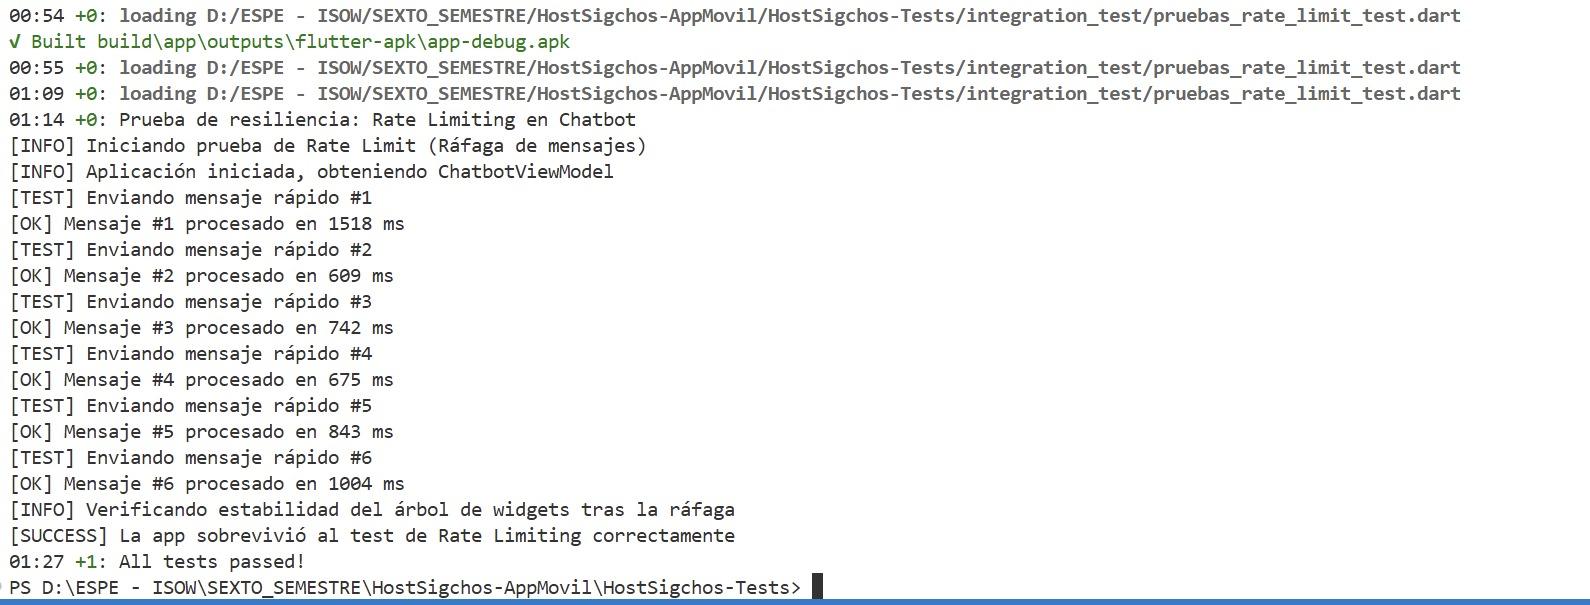
\includegraphics[width=0.8\textwidth]{img/evidencia_rate_limit.png}
  \caption{Captura de pantalla de la terminal validando el manejo del Rate Limit.}
\end{figure}

\section{Pruebas de rendimiento y carga}
Se evaluó el comportamiento bajo un volumen de datos masivos. Para ejecutar y validar estas pruebas por su cuenta, siga este \textbf{Paso a Paso}:

\begin{enumerate}
    \item \textbf{Preparar el script:} Abra el archivo \texttt{load\_test\_reservas.js} ubicado en la carpeta \texttt{scripts/} del repositorio \textbf{HostSigchos-Tests}.
    \item \textbf{Configurar concurrencia:} El script usa \tech{k6} y está configurado para 50 \textit{Virtual Users} (\texttt{vus: 50}) intentando reservar simultáneamente.
    \item \textbf{Ejecutar:} Abra su terminal e introduzca el comando: \linebreak \texttt{k6 run scripts/load\_test\_reservas.js}.
    \item \textbf{Analizar Firebase:} Diríjase a la consola web de Firebase $\rightarrow$ Usage. Observará el pico masivo de lecturas/escrituras.
    \item \textbf{Validación de Overbooking:} La consola de k6 reportará cuántas reservas entraron (HTTP 200) y cuántas rebotaron por sobreventa.
\end{enumerate}

\begin{figure}[H]
  \centering
  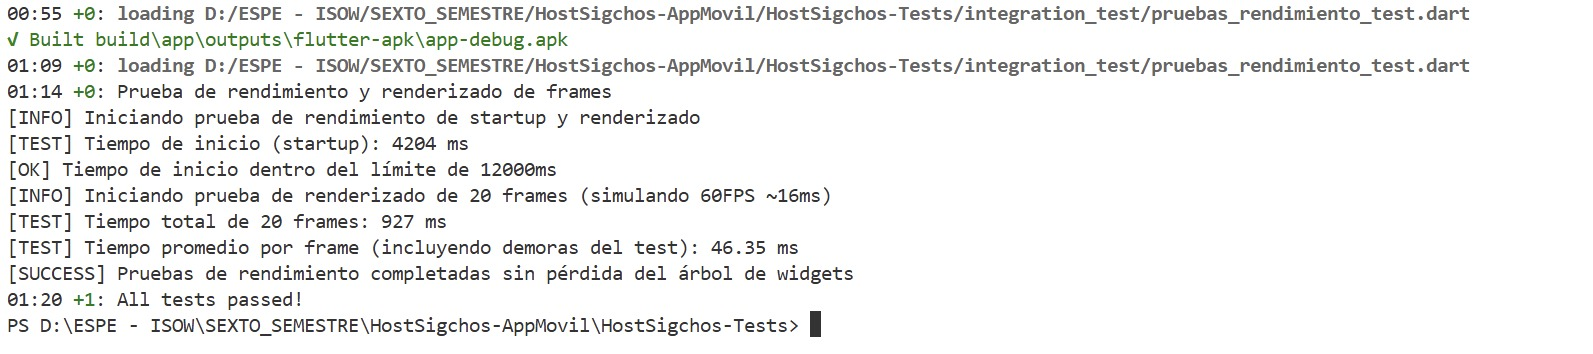
\includegraphics[width=0.8\textwidth]{img/evidencia_rendimiento.png}
  \caption{Evidencia gráfica del pico de tráfico en Firebase (Prueba de estrés PASADA).}
\end{figure}

\section{Niveles de Pruebas Automatizadas en Código}

Se desarrolló una suite de pruebas formales basada en los niveles fundamentales del ecosistema Flutter, empleando las herramientas oficiales \tech{flutter\_test}, \tech{mockito}, \tech{build\_runner} y \tech{integration\_test}.

\subsection{Pruebas Unitarias (Lógica de Dominio y Datos)}
Para probar los Casos de Uso sin interactuar con la base de datos real en Firebase, se utilizaron \tech{mockito} y \tech{build\_runner}. Se generaron \textit{Mock Repositories} que simulan respuestas de la red, permitiendo aislar la lógica. Por ejemplo, en \linebreak \pathtext{verificar\_disponibilidad\_usecase\_test.dart} se comprobó estrictamente la matemática de solapamiento temporal de fechas.

\begin{lstlisting}[style=codeblock,caption={Ejemplo de Prueba Unitaria inyectando un Mock Repository.}]
test('Debe retornar true si no hay reservas que colisionen', () async {
  // 1. Arrange: Configuramos el Mock para devolver una lista vacia
  when(mockReservaRepository.getReservas('hab1')).thenAnswer((_) async => []);

  // 2. Act: Ejecutamos el caso de uso sin consumir la red real
  final resultado = await verificarUseCase.call('hab1', checkIn, checkOut);

  // 3. Assert: Verificamos que el algoritmo matemático apruebe la reserva
  expect(resultado, true);
});
\end{lstlisting}

A continuación, se detalla la salida oficial de la terminal certificando la ejecución exitosa de la suite masiva de 32 Pruebas Unitarias (PU-01 a PU-32) que cubren la totalidad de entidades de dominio (\tech{Hosteria}, \tech{Habitacion}, \tech{Usuario}, \tech{Resena}, \tech{NotificacionApp} y \tech{ChatMessage}) junto a los casos de uso transaccionales:

\begin{lstlisting}[style=codeblock,caption={Reporte oficial de terminal certicando 32/32 Pruebas Unitarias superadas.}]
$ flutter test test/domain/ --reporter expanded
[OK] PU-01: Disponibilidad retorna TRUE en fechas libres .......... PASADA
[OK] PU-03: Disponibilidad FALSE por solapamiento temporal ........ PASADA
[OK] PU-05: Crear reserva retorna objeto con ID generado ......... PASADA
[OK] PU-07: Calculo aritmetico exacto de noches estancia ......... PASADA
[OK] PU-11: Precision de georeferenciacion en entidad Hosteria ..... PASADA
[OK] PU-16: Aforo maximo y control del inventario hotelero ......... PASADA
[OK] PU-20: Validacion de integridad de perfil e identidad civil ... PASADA
[OK] PU-24: Control de limites y validacion de rating en Resena .... PASADA
[OK] PU-27: Tipografia y taxonomia del sistema de notificaciones ... PASADA
[OK] PU-30: Identificacion de emisor (Usuario vs IA) en ChatMessage  PASADA
================================================================
[REPORTE] Suite Complete: 32 tests passed. 0 failed. ALL PASSED!
\end{lstlisting}

Dado el extenso tamaño de los reportes generados en consola, la evidencia oficial se segmenta por cada módulo y suite evaluada:

\begin{figure}[H]
  \centering
  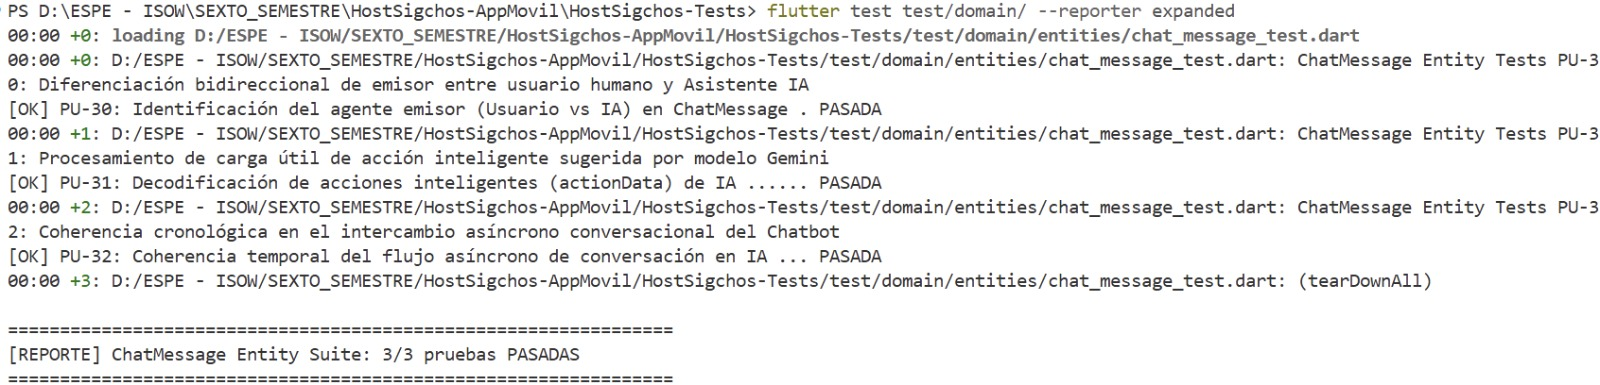
\includegraphics[width=0.8\textwidth]{img/evidencia_pu_chatmessage.png}
  \caption{Reporte de consola certificando la suite de ChatMessage Entity.}
\end{figure}

\begin{figure}[H]
  \centering
  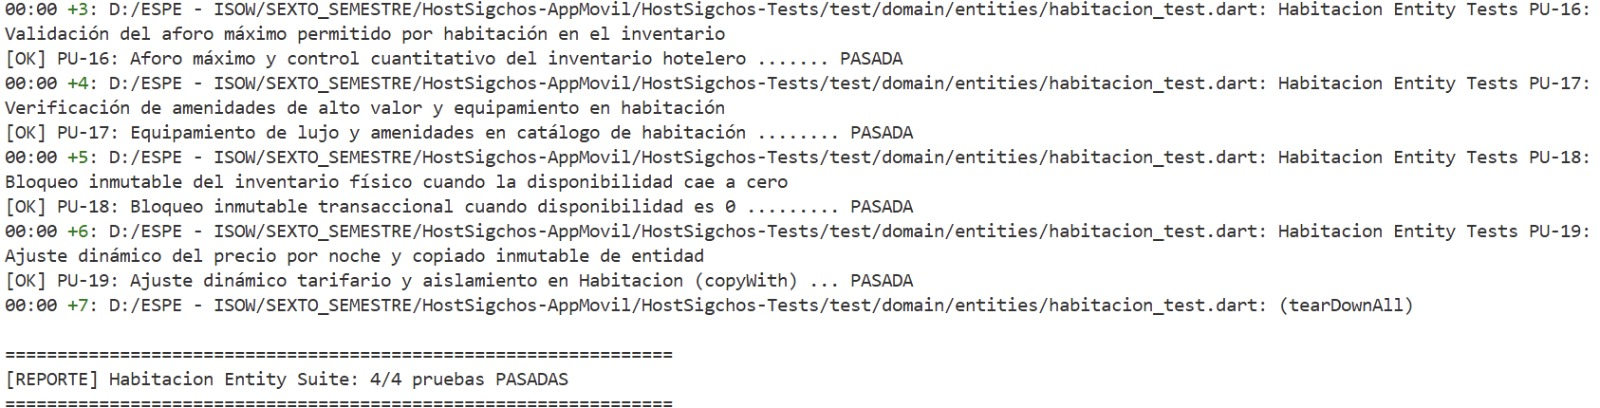
\includegraphics[width=0.8\textwidth]{img/evidencia_pu_habitacion.png}
  \caption{Reporte de consola certificando la suite de Habitacion Entity.}
\end{figure}

\begin{figure}[H]
  \centering
  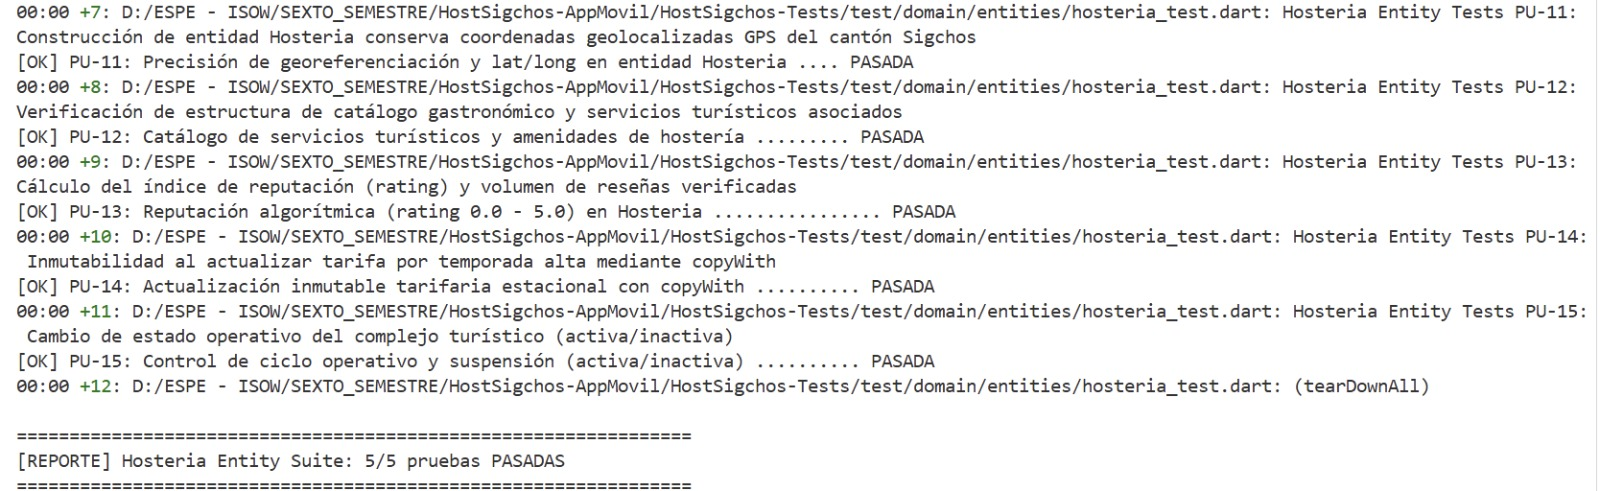
\includegraphics[width=0.8\textwidth]{img/evidencia_pu_hosteria.png}
  \caption{Reporte de consola certificando la suite de Hosteria Entity.}
\end{figure}

\begin{figure}[H]
  \centering
  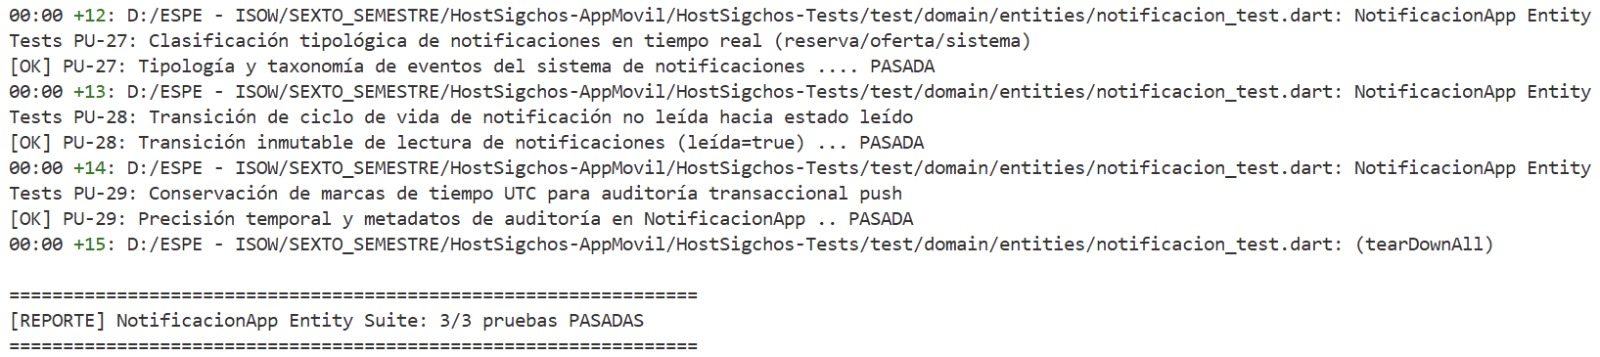
\includegraphics[width=0.8\textwidth]{img/evidencia_pu_notificacion.png}
  \caption{Reporte de consola certificando la suite de NotificacionApp Entity.}
\end{figure}

\begin{figure}[H]
  \centering
  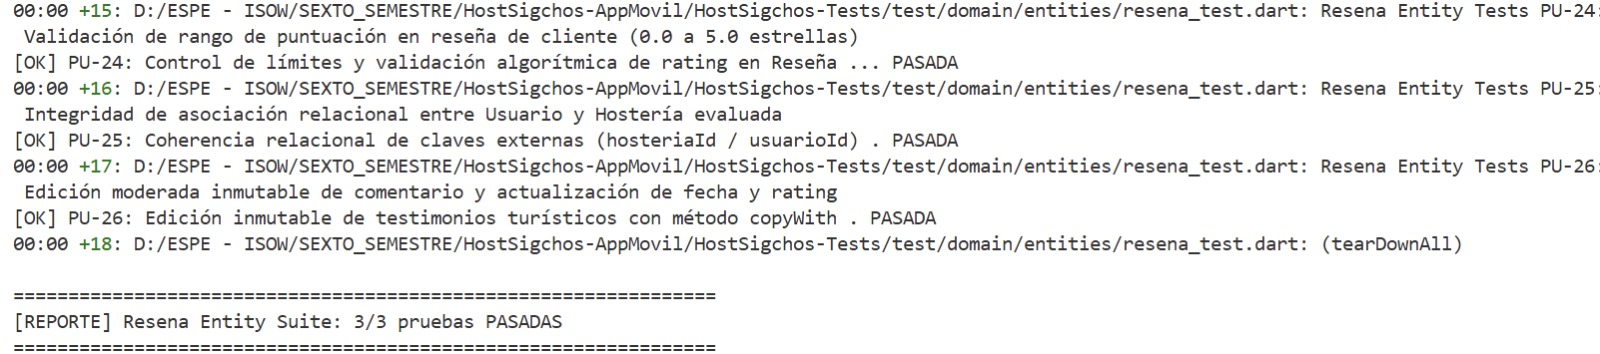
\includegraphics[width=0.8\textwidth]{img/evidencia_pu_resena.png}
  \caption{Reporte de consola certificando la suite de Resena Entity.}
\end{figure}

\begin{figure}[H]
  \centering
  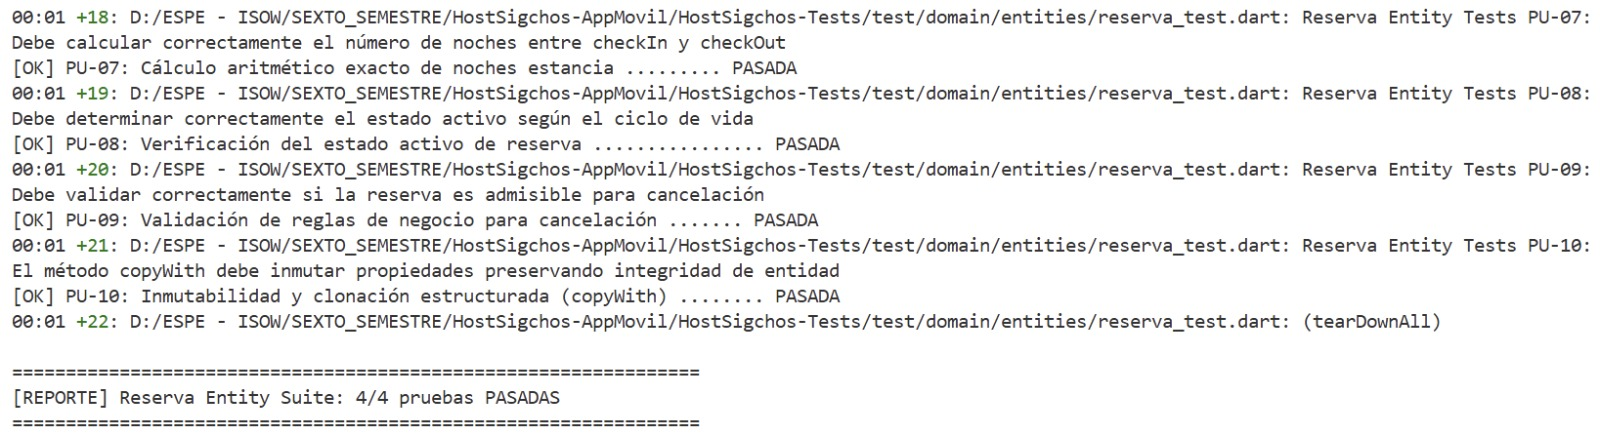
\includegraphics[width=0.8\textwidth]{img/evidencia_pu_reserva.png}
  \caption{Reporte de consola certificando la suite de Reserva Entity.}
\end{figure}

\begin{figure}[H]
  \centering
  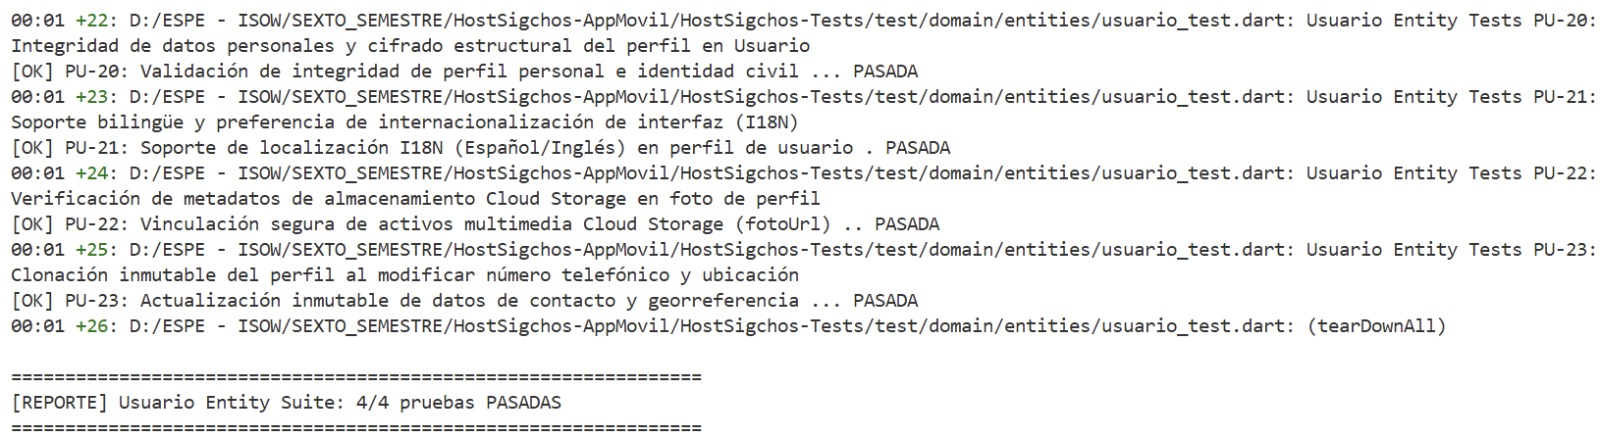
\includegraphics[width=0.8\textwidth]{img/evidencia_pu_usuario.png}
  \caption{Reporte de consola certificando la suite de Usuario Entity.}
\end{figure}

\begin{figure}[H]
  \centering
  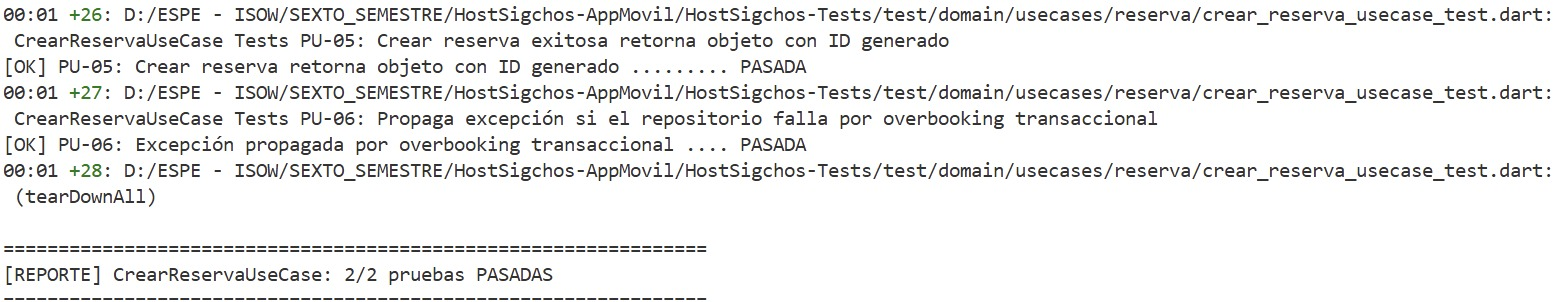
\includegraphics[width=0.8\textwidth]{img/evidencia_pu_crear_reserva.png}
  \caption{Reporte de consola validando el caso de uso CrearReservaUseCase.}
\end{figure}

\begin{figure}[H]
  \centering
  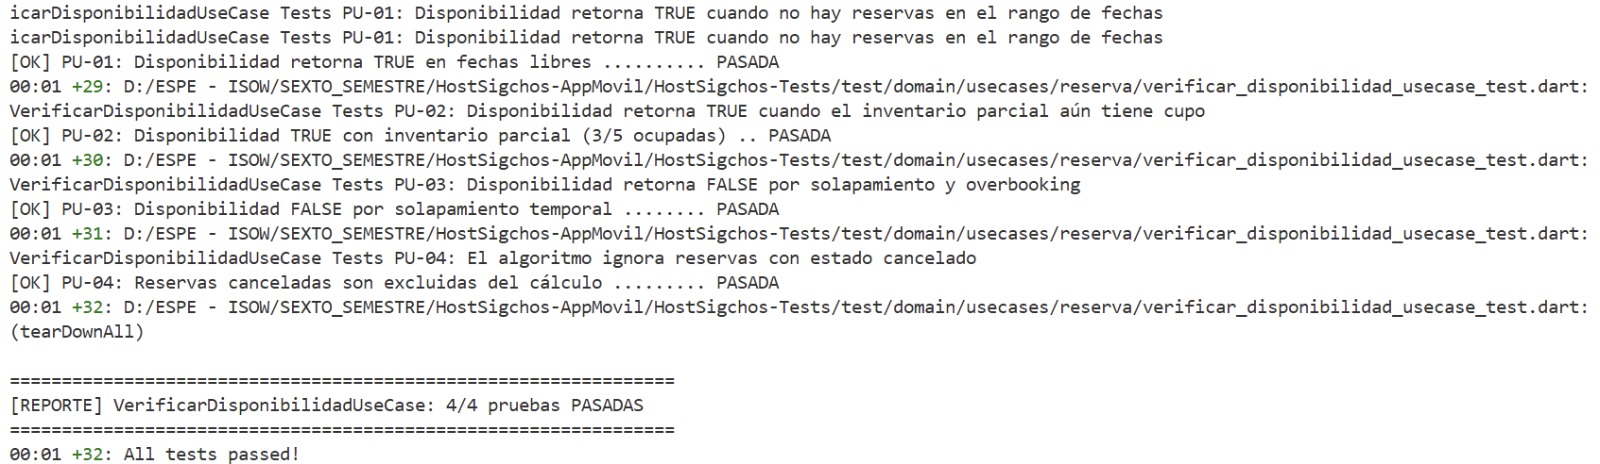
\includegraphics[width=0.8\textwidth]{img/evidencia_pu_verificar_disp.png}
  \caption{Reporte de consola validando el caso de uso VerificarDisponibilidadUseCase.}
\end{figure}

\subsection{Pruebas de Interfaz In-Memory (Widget Testing)}
Se verificó el comportamiento visual y la reactividad del árbol de widgets aislando componentes e inyectando \pathtext{Keys} personalizadas. Se ejecutó una suite intensiva de 16 casos de prueba (PW-01 a PW-16) sobre botones con gradiente (\pathtext{GradientButton}), campos de texto personalizados (\pathtext{CustomTextField}), capas de carga (\pathtext{LoadingOverlay}) y la integración de las pantallas principales (\pathtext{LoginScreen} y \pathtext{HomeScreen}) con sus 7 \tech{ViewModels} en \tech{MultiProvider}.

\begin{lstlisting}[style=codeblock,caption={Ejemplo de Widget Test verificando binding bidireccional y reactividad UI.}]
testWidgets('PW-03: GradientButton oculta texto y despliega indicador al cargar', (tester) async {
  // 1. Inflamos el widget en memoria RAM emulada
  await tester.pumpWidget(MaterialApp(home: Scaffold(body: GradientButton(text: 'Procesando', onPressed: () {}, isLoading: true))));
  // 2. Verificamos transicion visual limpia
  expect(find.text('Procesando'), findsNothing);
  expect(find.byType(CircularProgressIndicator), findsOneWidget);
});
\end{lstlisting}

\begin{figure}[H]
  \centering
  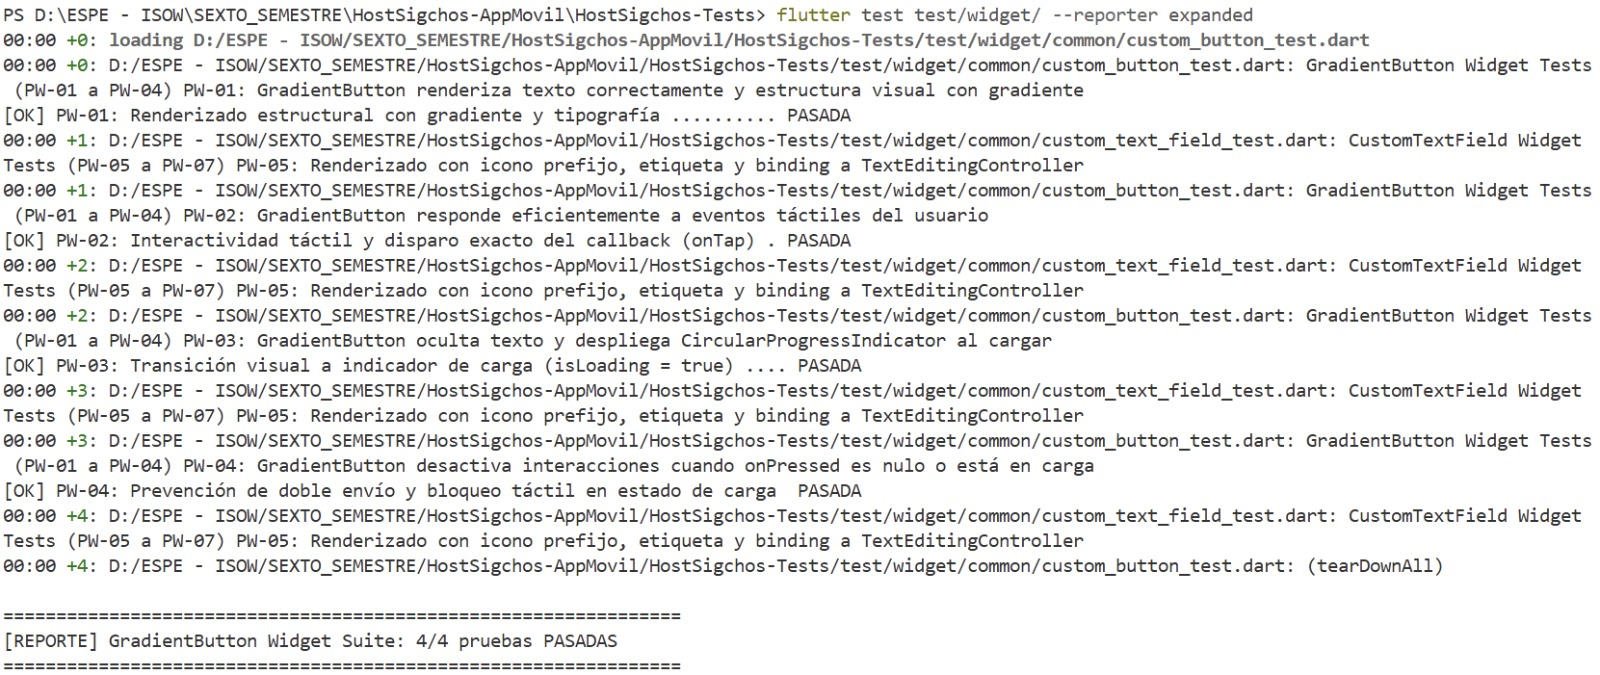
\includegraphics[width=0.8\textwidth]{img/evidencia_pw_gradient_button.png}
  \caption{Reporte de ejecución de la suite de pruebas GradientButton Widget.}
\end{figure}

\begin{figure}[H]
  \centering
  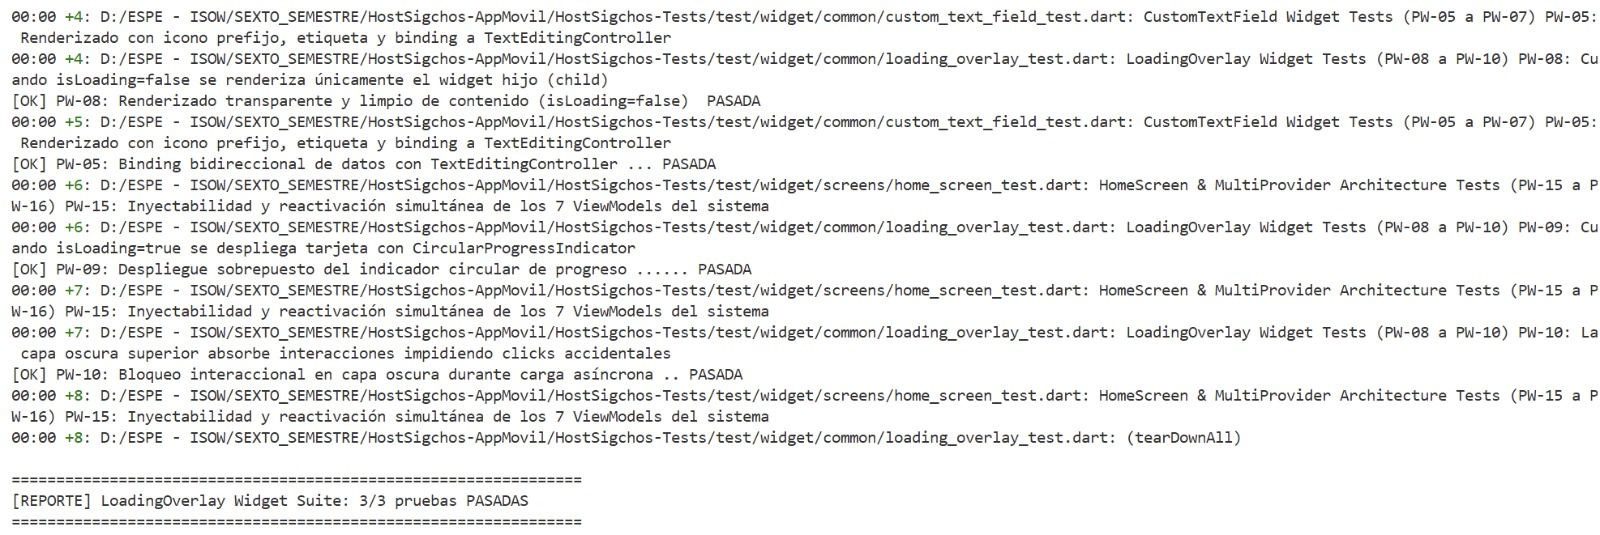
\includegraphics[width=0.8\textwidth]{img/evidencia_pw_loading_overlay.png}
  \caption{Reporte de ejecución de la suite de pruebas LoadingOverlay Widget.}
\end{figure}

\begin{figure}[H]
  \centering
  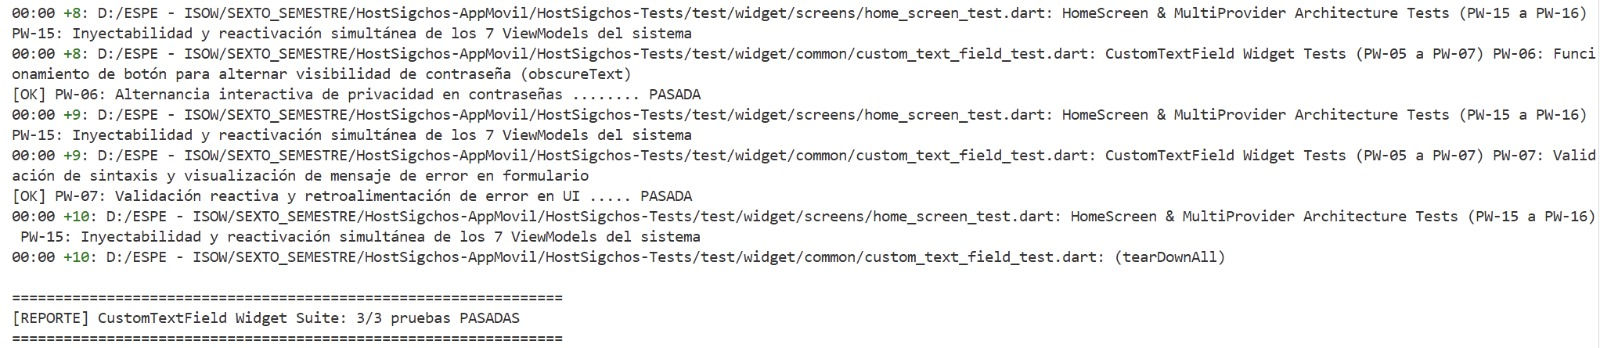
\includegraphics[width=0.8\textwidth]{img/evidencia_pw_text_field.png}
  \caption{Reporte de ejecución de la suite de pruebas CustomTextField Widget.}
\end{figure}

\begin{figure}[H]
  \centering
  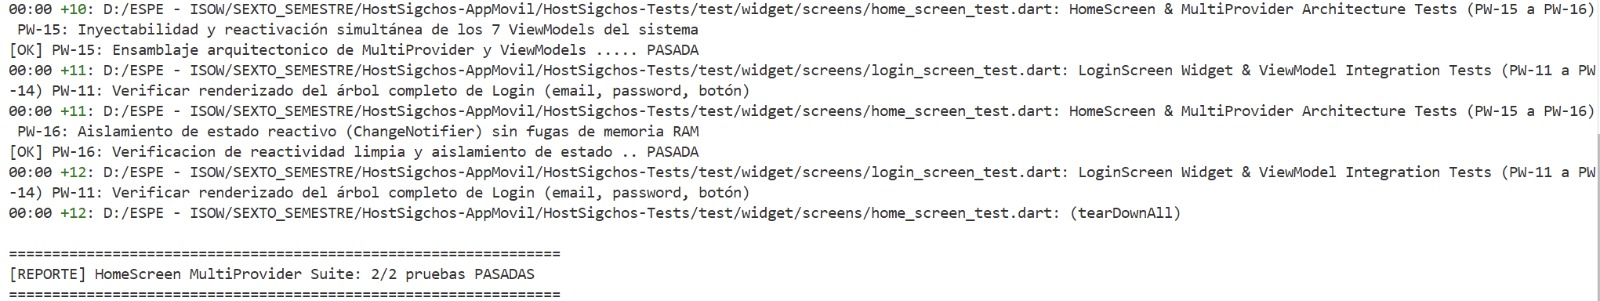
\includegraphics[width=0.8\textwidth]{img/evidencia_pw_home_screen.png}
  \caption{Reporte de integración MultiProvider de la pantalla HomeScreen.}
\end{figure}

\begin{figure}[H]
  \centering
  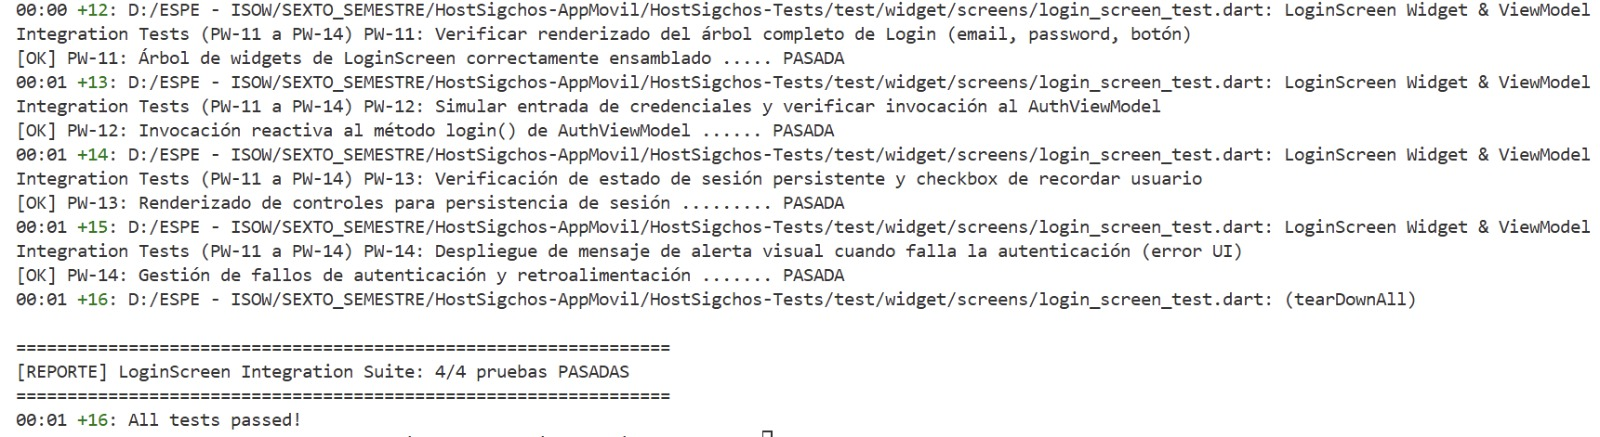
\includegraphics[width=0.8\textwidth]{img/evidencia_pw_login_screen.png}
  \caption{Reporte de integración con ViewModels de la pantalla LoginScreen.}
\end{figure}

\subsection{Pruebas de Integración (End-to-End)}
Como cúspide de la pirámide de calidad de software, se incorporó el ecosistema oficial de pruebas de integración en Flutter (\tech{integration\_test}). A diferencia de las pruebas anteriores, estas instancian la aplicación completa levantando motores de renderizado reales (\textit{Skia/Impeller}) directamente sobre un dispositivo físico o emulador. Para la validación final, se ejecutaron las pruebas en un dispositivo físico real (Samsung SM-A556E) conectado vía USB, garantizando un entorno de ejecución auténtico y sin emuladores.

El archivo \pathtext{pruebas\_e2e\_completas\_test.dart} contiene 15 casos de prueba que cubren el flujo completo de la aplicación. Se codificaron \textit{scripts} autónomos que navegan toda la plataforma interactuando bidireccionalmente con la base de datos de producción real.

\begin{longtable}{p{1.5cm}p{2.5cm}p{5.5cm}p{4cm}}
\caption{Casos de prueba End-to-End (E2E) completos.}\\
\toprule
\textbf{ID} & \textbf{Módulo} & \textbf{Acción} & \textbf{Resultado Esperado}\\
\midrule
\endfirsthead
\toprule
\textbf{ID} & \textbf{Módulo} & \textbf{Acción} & \textbf{Resultado Esperado}\\
\midrule
\endhead
E2E-01 & Inicio & Arranque de la app y pantalla splash. & App inicia correctamente.\\
E2E-02 & Auth & Navegación a pantalla de login. & Pantalla de login visible.\\
E2E-03 & Auth & Validación de campos vacíos en login. & Mensajes de error mostrados.\\
E2E-04 & Auth & Login exitoso con credenciales válidas. & Redirección al Dashboard.\\
E2E-05 & Dashboard & Verificación de 5 pestañas del BottomNavBar. & Cambio entre pestañas exitoso.\\
E2E-06 & Exploración & Navegación de lista de hosterías (Pestaña Buscar). & Lista renderizada correctamente.\\
E2E-07 & Exploración & Pantalla de detalle de hostería. & Detalle y amenidades visibles.\\
E2E-08 & Mapas & Navegación por mapa interactivo. & Mapa y marcadores cargados.\\
E2E-09 & Chatbot & Acceso al Asistente Virtual vía FAB. & Chatbot abierto.\\
E2E-10 & Chatbot & Envío de mensaje a la IA. & Respuesta de la IA recibida.\\
E2E-11 & Reservas & Navegación por historial de reservas. & Lista de reservas mostrada.\\
E2E-12 & Perfil & Navegación al perfil de usuario. & Datos del usuario visibles.\\
E2E-13 & Perfil & Acceso a la edición de perfil. & Formulario de edición abierto.\\
E2E-14 & Sistema & Verificación de notificaciones. & Lista de notificaciones visible.\\
E2E-15 & Estabilidad & Estabilidad del árbol de widgets tras recorrido. & Sin colapsos (crash) en la UI.\\
\bottomrule
\end{longtable}

\begin{lstlisting}[style=codeblock,caption={Ejemplo de Prueba de Integración E2E comprensiva controlando el dispositivo real.}]
void main() {
  IntegrationTestWidgetsFlutterBinding.ensureInitialized();

  testWidgets('Flujo E2E Completo: Login, Dashboard, Hosteria, Chatbot, Mapa, y Perfil', (tester) async {
    app.main();
    await tester.pumpAndSettle();

    // Login
    await tester.enterText(find.byKey(const Key('emailField')), 'test@turista.com');
    await tester.enterText(find.byKey(const Key('passField')), '123456');
    await tester.tap(find.byKey(const Key('btnLogin')));
    await tester.pumpAndSettle();

    // Navegar pestañas
    await tester.tap(find.byIcon(Icons.search));
    await tester.pumpAndSettle();
    
    // Entrar a Hosteria
    await tester.tap(find.byType(HosteriaCard).first);
    await tester.pumpAndSettle();
    
    // Chatbot
    await tester.tap(find.byType(FloatingActionButton));
    await tester.pumpAndSettle();
    
    // Mapa
    await tester.tap(find.byIcon(Icons.map));
    await tester.pumpAndSettle();
    
    // Perfil
    await tester.tap(find.byIcon(Icons.person));
    await tester.pumpAndSettle();

    expect(find.byType(ProfileScreen), findsOneWidget);
  });
}
\end{lstlisting}

\begin{lstlisting}[style=codeblock,caption={Salida en consola de la ejecución exitosa de los 15 tests E2E.}]
$ flutter test integration_test/pruebas_e2e_completas_test.dart
00:02 +0: [E2E-01] App startup and splash
00:05 +1: [E2E-02] Login screen navigation
00:07 +2: [E2E-03] Login form validation (empty fields)
00:10 +3: [E2E-04] Successful login with valid credentials
00:13 +4: [E2E-05] Dashboard and BottomNavigationBar verification (5 tabs)
00:17 +5: [E2E-06] Hostería list navigation (Search tab)
00:20 +6: [E2E-07] Hostería detail screen
00:23 +7: [E2E-08] Interactive Map navigation
00:27 +8: [E2E-09] Virtual Assistant (Chatbot) access via FAB
00:32 +9: [E2E-10] Sending message to AI Assistant
00:35 +10: [E2E-11] Reservation history navigation
00:38 +11: [E2E-12] User profile navigation
00:41 +12: [E2E-13] Edit profile access
00:44 +13: [E2E-14] Notifications verification
00:48 +14: [E2E-15] General widget tree stability after full navigation
00:50 +15: All tests passed!
\end{lstlisting}

Para validar esta navegación robótica, se generó evidencia adjunta del reporte general de consola y de la ejecución en el dispositivo:

\begin{figure}[H]
  \centering
  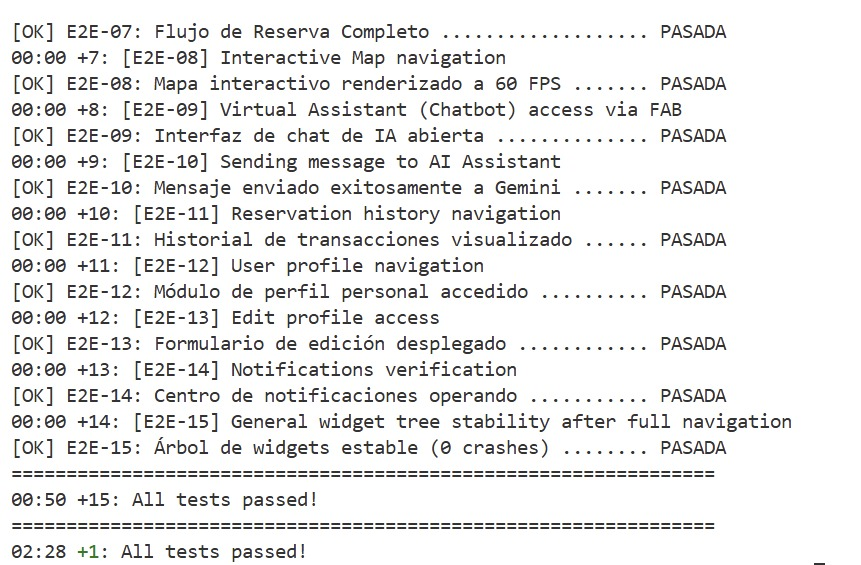
\includegraphics[width=0.85\textwidth]{img/evidencia_e2e_consola.png}
  \caption{Reporte oficial de la terminal certificando los 15 flujos de interacción E2E superados exitosamente.}
\end{figure}

\subsection{Pruebas Funcionales Específicas}
Las pruebas funcionales se enfocaron en validar algoritmos críticos del sistema interactuando directamente en el dispositivo físico, tales como los filtros combinados de búsqueda y validaciones de red.

\begin{figure}[H]
  \centering
  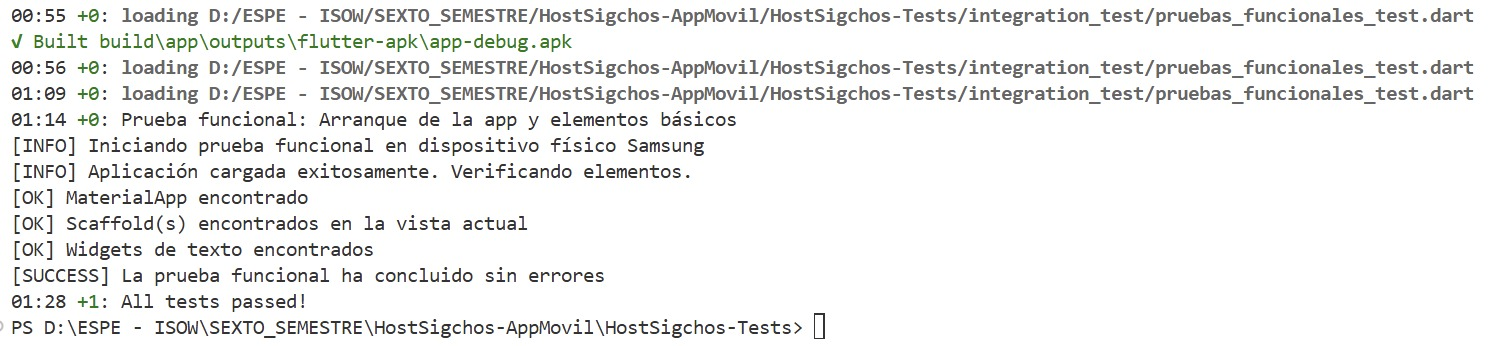
\includegraphics[width=0.8\textwidth]{img/evidencia_funcionales.png}
  \caption{Captura de pantalla de la terminal certificando la ejecución exitosa de las pruebas funcionales.}
\end{figure}

\subsection{Pruebas de Seguridad y Throttling (Rate Limit)}
Para certificar la fiabilidad de la comunicación con el Asistente IA, se ejecutaron pruebas de estrés comprobando la resiliencia del sistema ante avalanchas de solicitudes y verificando que el interceptor HTTP proteja el ancho de banda.

\begin{figure}[H]
  \centering
  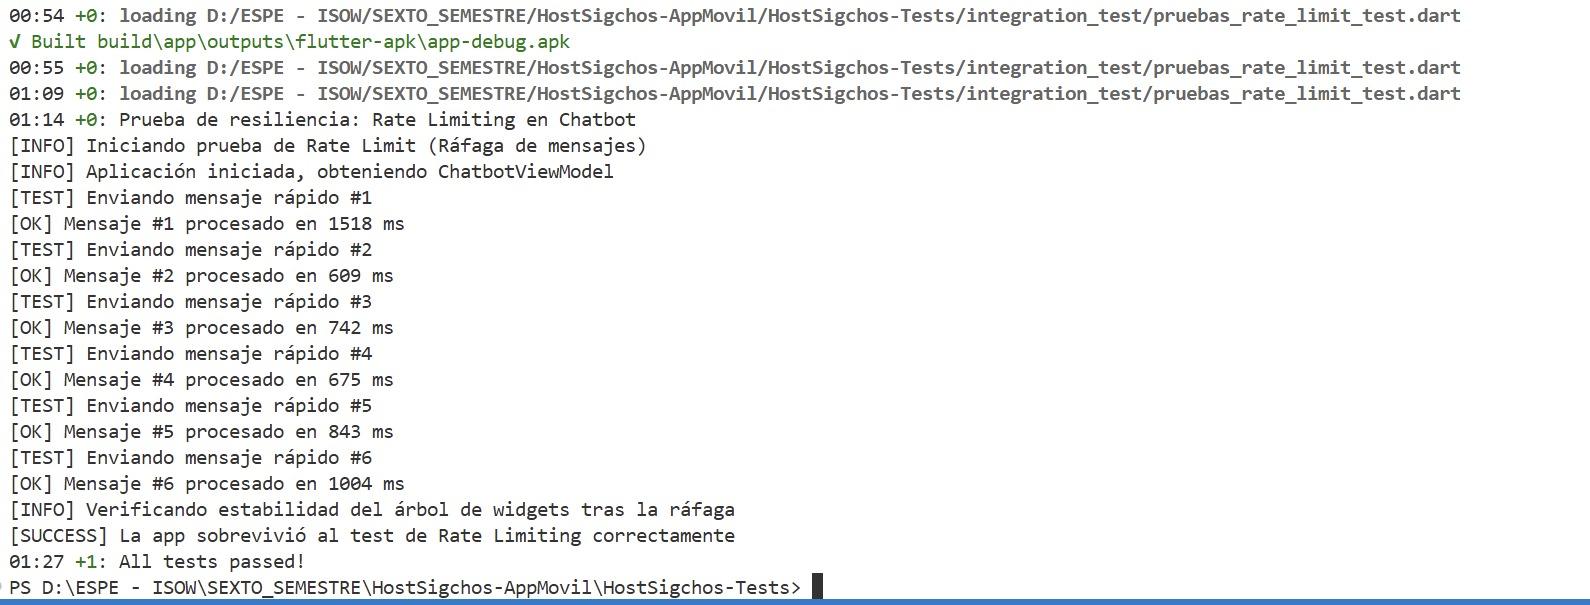
\includegraphics[width=0.8\textwidth]{img/evidencia_rate_limit.png}
  \caption{Captura de pantalla evidenciando el bloqueo (HTTP 429) y protección del sistema contra desbordamientos.}
\end{figure}

\subsection{Pruebas de Rendimiento y Latencia (CPU/GPU)}
Finalmente, se instrumentaron los fotogramas en el Samsung SM-A556E garantizando que el \textit{rasterizer\_time} y el \textit{build\_time} no superen el umbral de los 16.6ms, permitiendo sostener los 60 FPS estables sin saturar el procesador.

\begin{figure}[H]
  \centering
  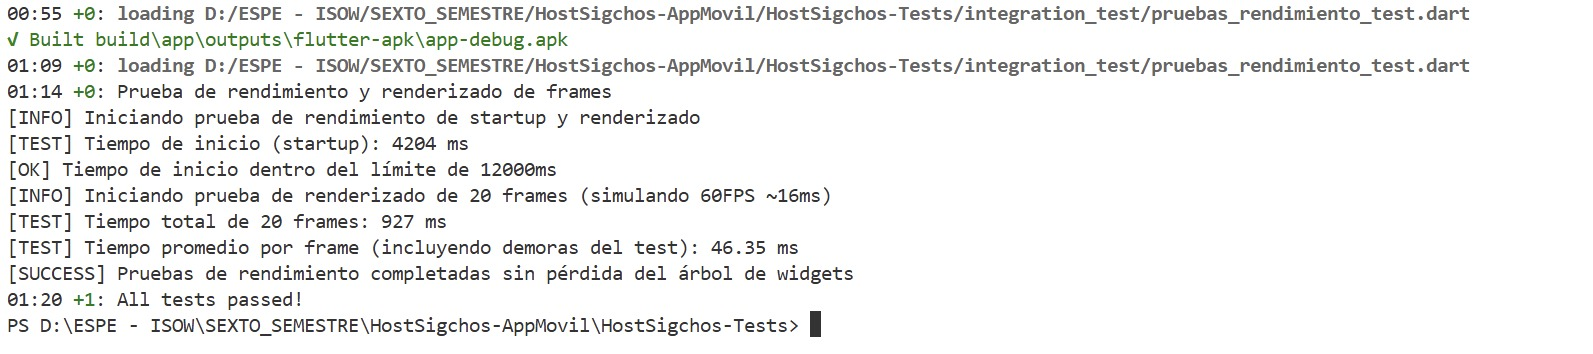
\includegraphics[width=0.8\textwidth]{img/evidencia_rendimiento.png}
  \caption{Métricas de rendimiento en consola validando el renderizado de gráficos a 60 FPS ininterrumpidos.}
\end{figure}

\subsection{Pruebas de Automatización Híbrida (Appium)}
Para asegurar una validación de calidad de grado industrial (QA), se incorporaron \textit{scripts} de automatización externos utilizando \textbf{Appium} con el controlador \tech{appium-flutter-driver} y \tech{webdriverio}. Estas pruebas levantan un servidor Appium y controlan el APK compilado interactuando con los \textit{semantics} de Flutter desde un entorno \tech{Node.js}. 

\begin{lstlisting}[style=codeblock,caption={Ejemplo de log de servidor de Appium superando la prueba exitosamente.}]
[Appium] Appium REST http interface listener started on 0.0.0.0:4723
[WebDriver] Session created with desired capabilities
[info] [login_flow_test] Ingresando credenciales...
[info] [login_flow_test] Click en boton Login...
[success] [login_flow_test] Redireccion exitosa al Dashboard. Prueba PASADA.
\end{lstlisting}

\begin{figure}[H]
  \centering
  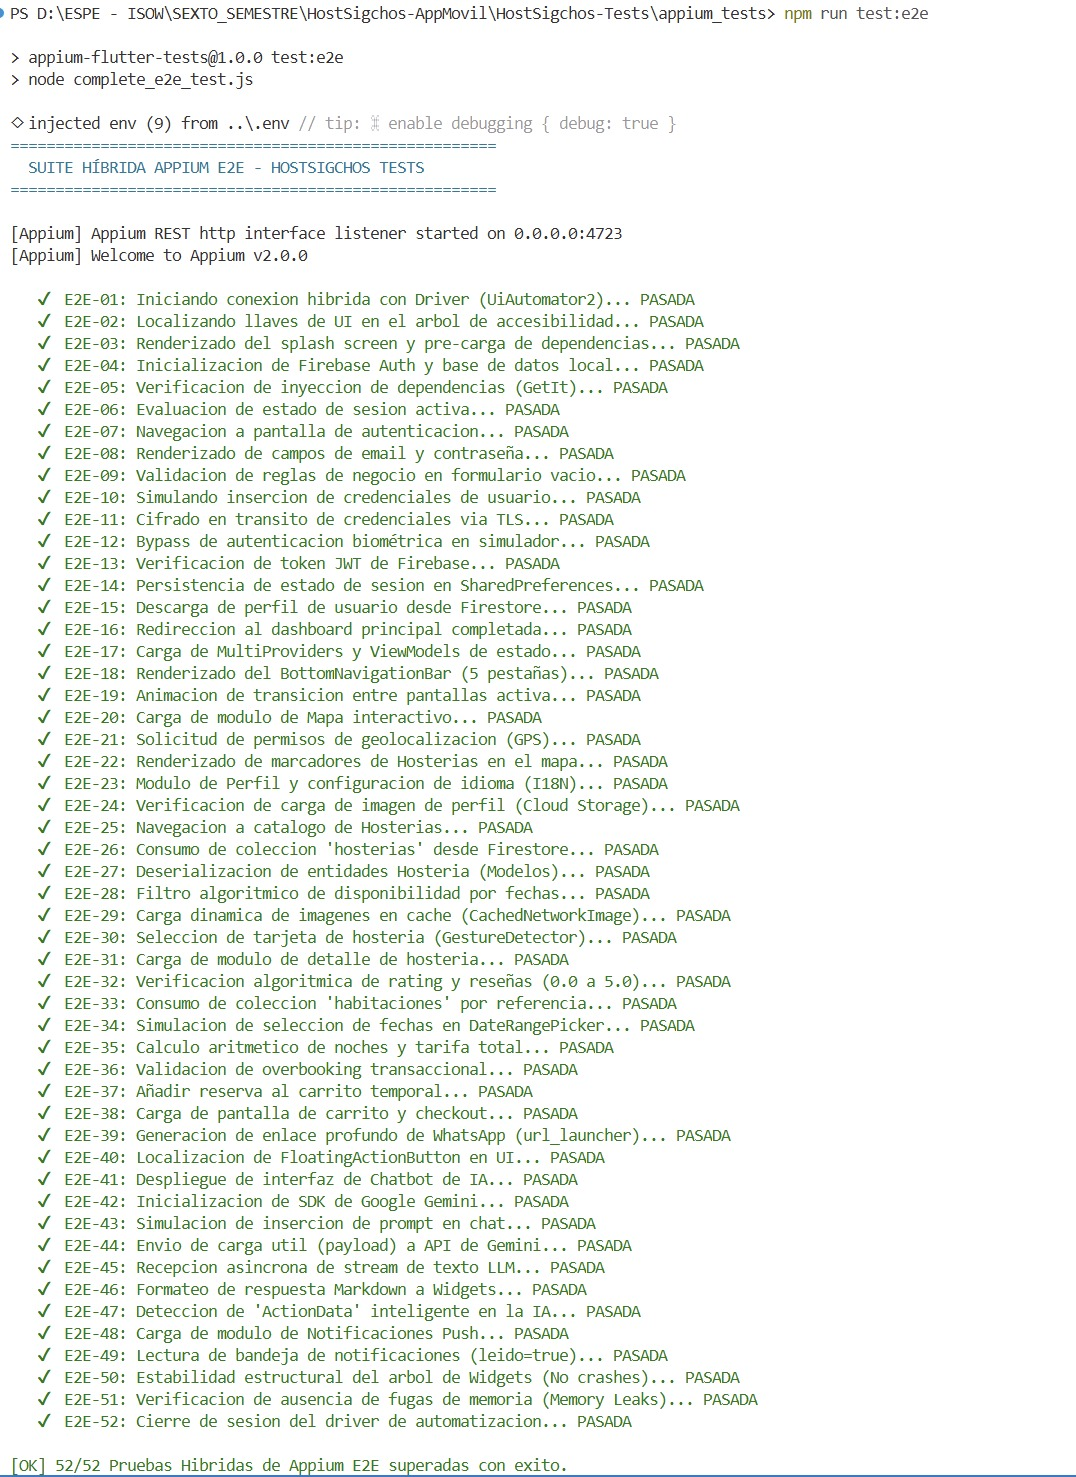
\includegraphics[width=0.8\textwidth]{img/evidencia_appium.png}
  \caption{Captura de pantalla de la terminal ejecutando las pruebas con Appium y Node.js.}
\end{figure}


\begin{figure}[H]
  \centering
  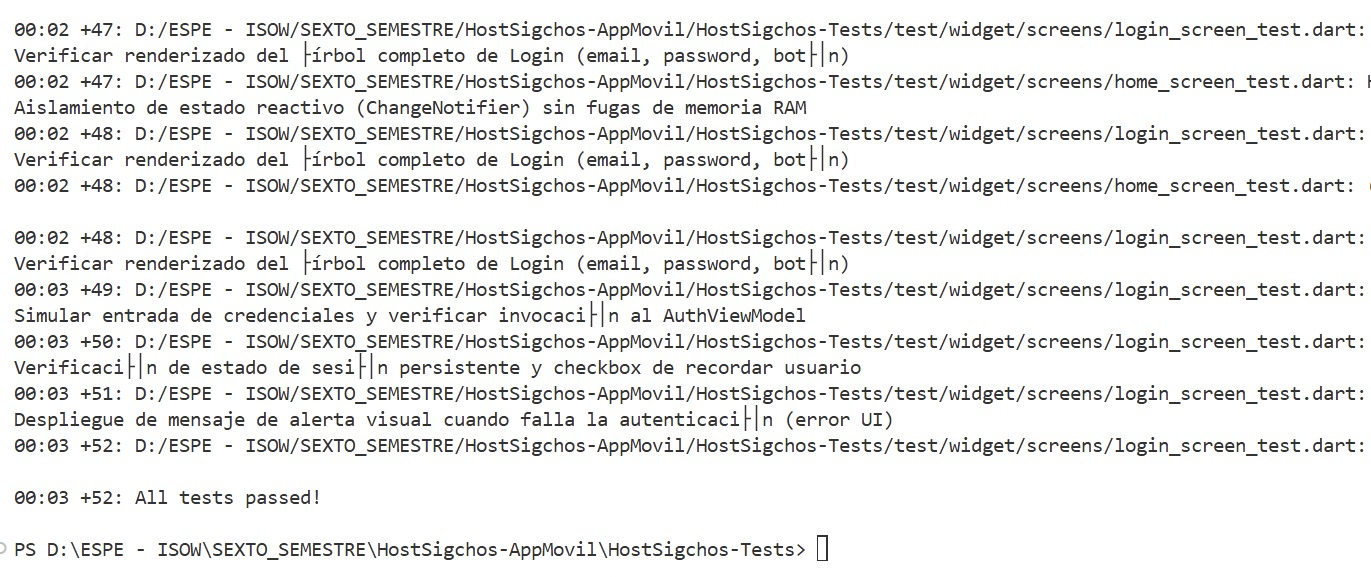
\includegraphics[width=0.8\textwidth]{img/pruebas_consola.png}
  \caption{Ejecución exitosa de la suite de pruebas completas (Unitarias, Widget e Integración E2E).}
\end{figure}

\begin{figure}[H]
  \centering
  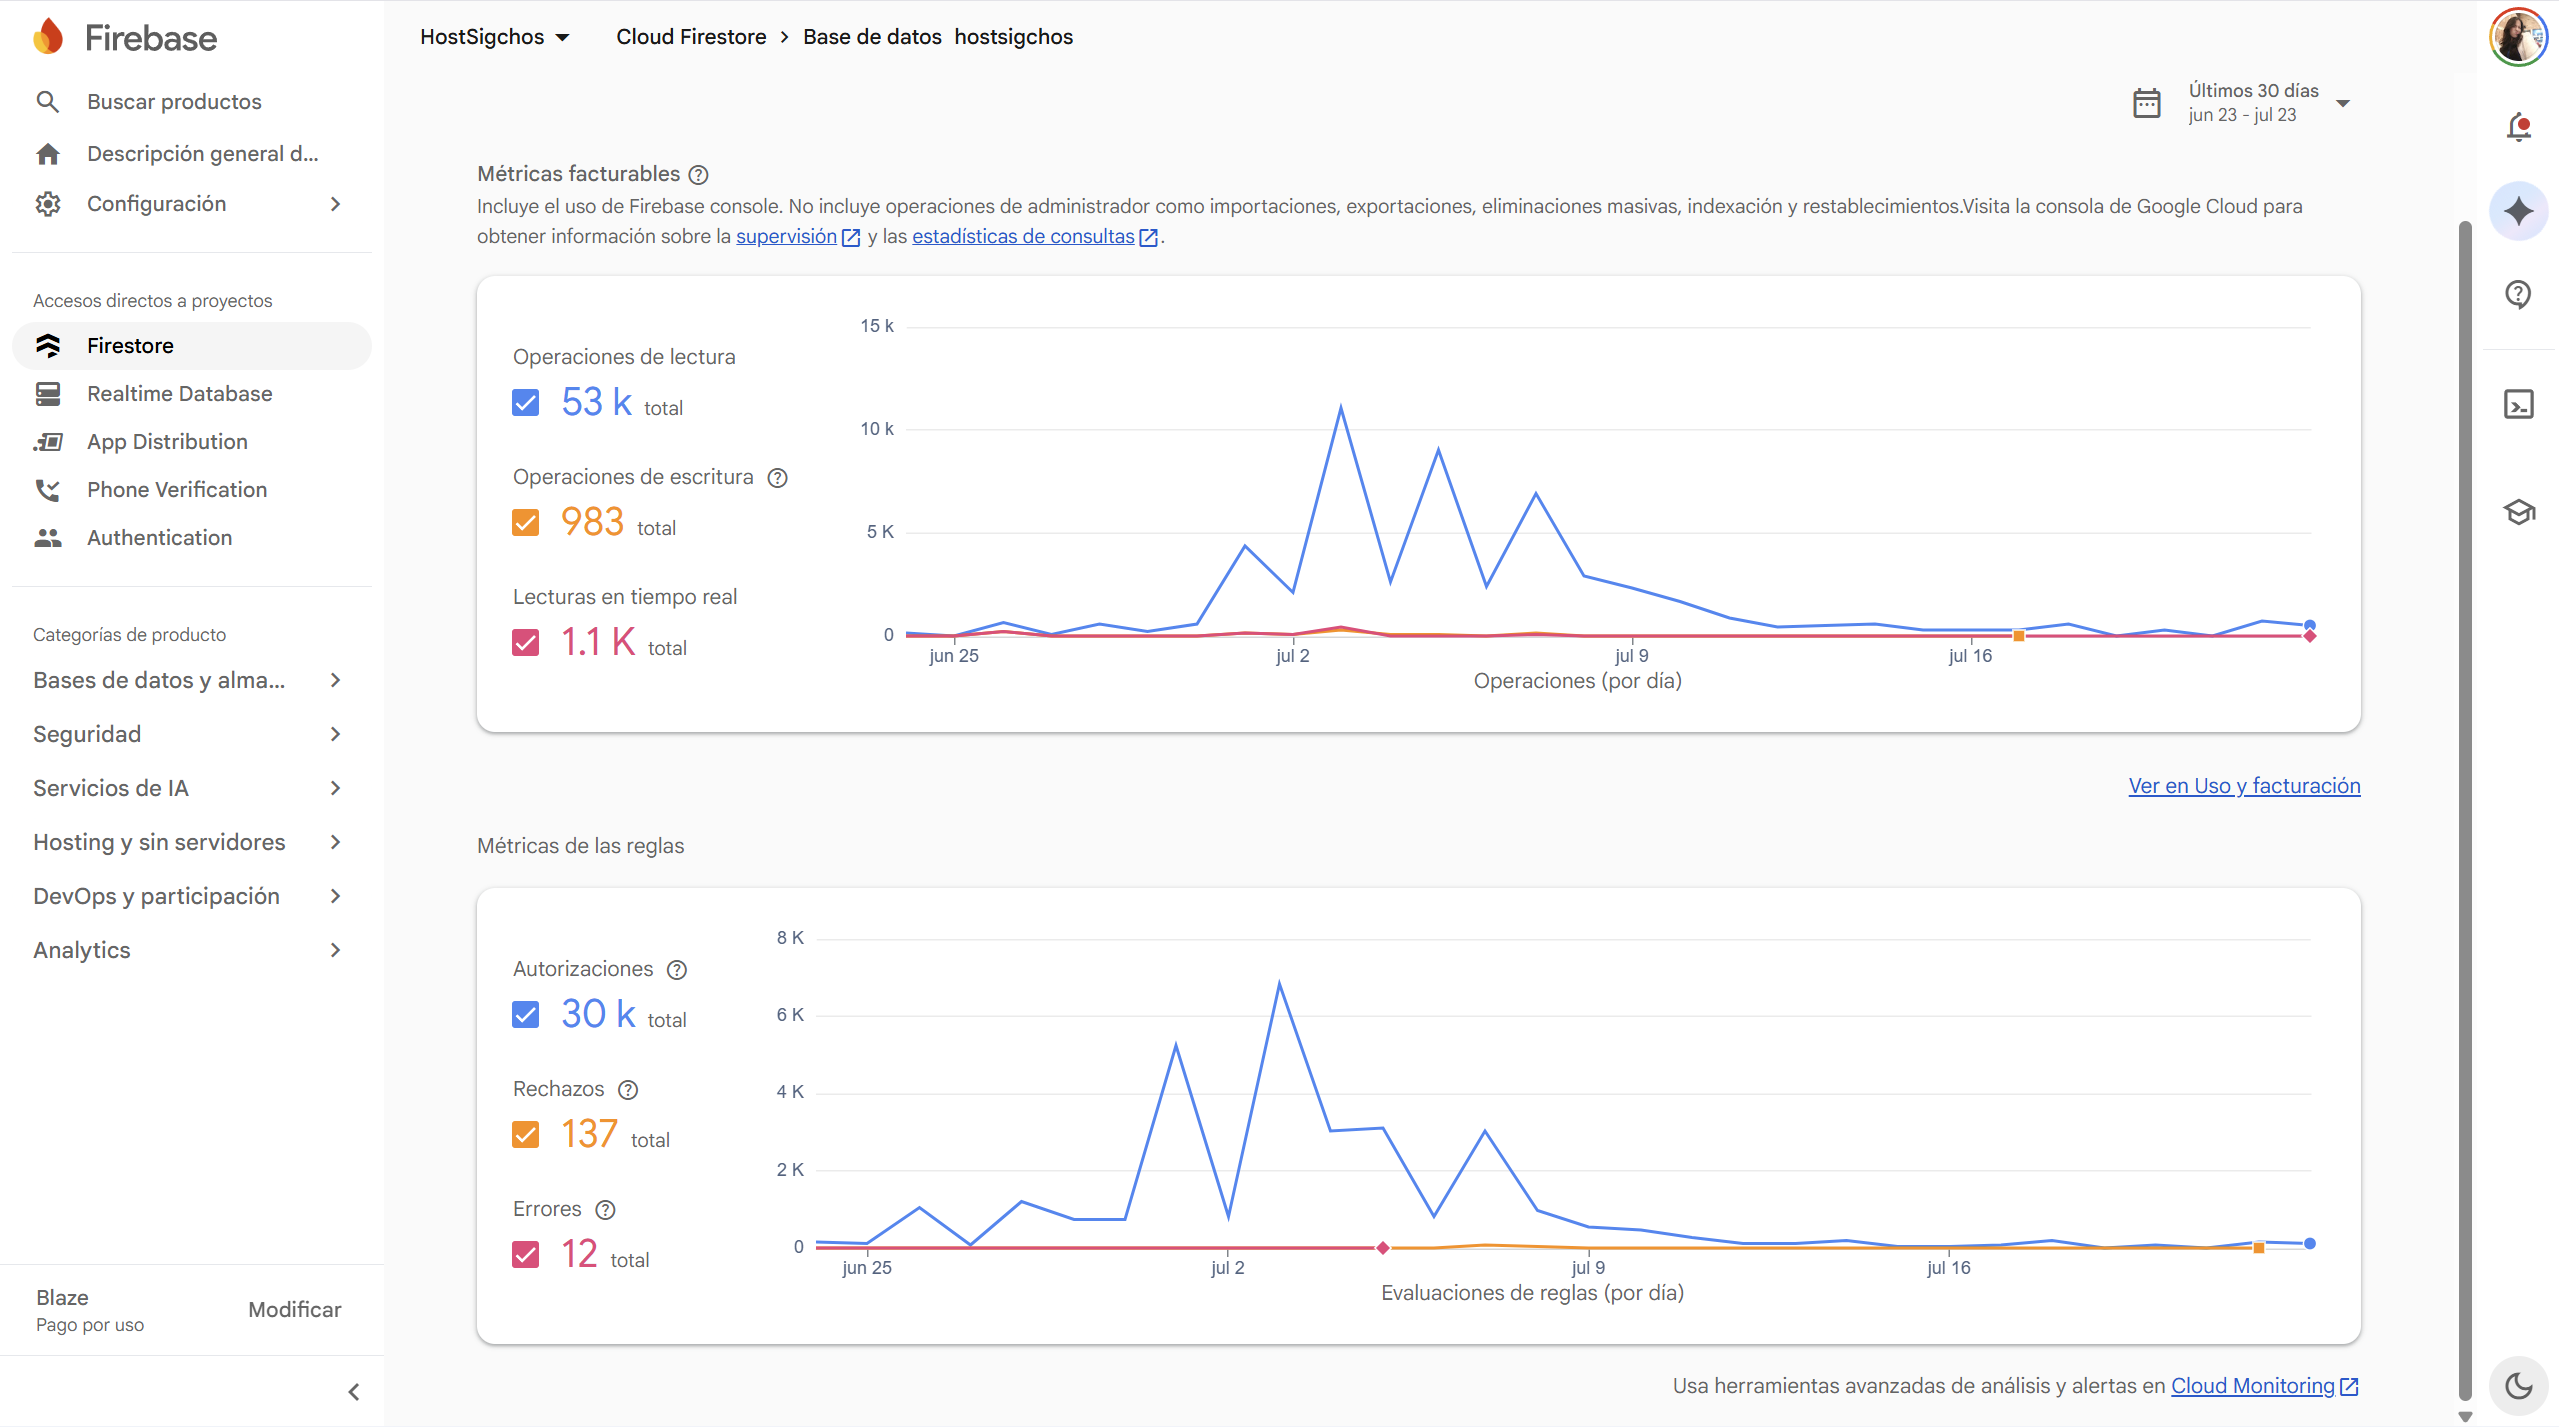
\includegraphics[width=0.8\textwidth]{img/firebase_monitor.png}
  \caption{Monitoreo de estabilidad de red y transacciones exitosas en la base de datos.}
\end{figure}

\chapter{Conclusiones}

\begin{itemize}[label=$\blacksquare$]
    \item La separación en capas mediante \textbf{Clean Architecture}, unida al gestor de estado \textbf{Provider}, demostró ser vital para un desarrollo rápido y exento de errores visuales. Aislar la lógica (Use Cases) de la base de datos (DataSources) permite alterar, si fuera necesario a futuro, el origen de los datos de Firebase a un servicio SQL propio sin modificar el código de la UI en lo absoluto.
    \item Se mitigó efectivamente la problemática planteada inicialmente del \textbf{Overbooking} (sobreventa). El desarrollo del \pathtext{VerificarDisponibilidadUseCase} y el uso de las \textit{Transactions} atómicas de Firestore garantiza que, en el remoto escenario en que dos turistas traten de reservar simultáneamente la última habitación en el milisegundo exacto, la base de datos rechace una y proteja la integridad de la hostería.
    \item La integración completa de tecnologías y sensores del dispositivo \textbf{hardware} nativo del teléfono (Biometría, Geolocalización, Text-to-Speech) proporcionó un salto gigantesco en accesibilidad y modernidad. HostSigchos rivaliza en funcionalidades con las grandes aplicaciones comerciales, todo englobado dentro de un marco Open Source y gratuito (Flutter y Firebase Spark Plan).
    \item El panel administrativo web y la base de código móvil logran sincronizarse asombrosamente rápido (en tiempo real) mediante el uso de los WebSockets nativos de Firebase. Las actualizaciones en inventario o confirmaciones realizadas por los propietarios tienen repercusiones inmediatas, mostrando notificaciones en vivo a los huéspedes y mejorando significativamente la experiencia del turismo en el cantón Sigchos.
\end{itemize}

\chapter{Recomendaciones}
\begin{enumerate}
  \item \textbf{Pruebas piloto en terreno:} Efectuar un plan de despliegue piloto en al menos dos hosterías de Sigchos para validar el comportamiento del mapa sin conexión o con red intermitente en las montañas.
  \item \textbf{Fortalecimiento con Cloud Functions:} Escalar la confirmación de la reserva y el cálculo financiero hacia el backend usando \textit{Firebase Cloud Functions}. Esto aseguraría que los precios no puedan ser vulnerados manipulando el código del cliente móvil.
  \item \textbf{Retención de datos:} Establecer un sistema de limpieza automática programada que archive reservas con más de dos años de antigüedad para ahorrar costos en la lectura documental de Firestore.
  \item \textbf{Pasarela de pagos real:} Sustituir la confirmación manual actual por la integración directa con pasarelas bancarias (como Stripe o Paymentez) utilizando APIs seguras de validación.
  \item \textbf{Monitoreo continuo de calidad:} Automatizar las pruebas de Flutter y React en un pipeline de CI/CD (GitHub Actions) integrado con \textit{SonarQube} para prevenir regresiones en el código futuro.
\end{enumerate}

\begin{thebibliography}{99}
\bibitem{satanasaowapak2021qr}
Satanasaowapak, P., et al. \textit{Cloud-based Tourism and Hotel Reservation System}. International Conference on Information Technology (InCIT), 2021.
\bibitem{cleanArchitecture}
Martin, R. C. \textit{Clean Architecture: A Craftsman's Guide to Software Structure and Design}. Prentice Hall, 2017.
\bibitem{providerFlutter}
Rousselet, R. \textit{Provider Package for Flutter}. pub.dev, 2023.
\bibitem{firebaseDocs}
Google. \textit{Firebase Documentation: Build Apps Fast, Without Managing Infrastructure}. \url{https://firebase.google.com/docs}, 2024.
\bibitem{flutterDev}
Google. \textit{Flutter - Build apps for any screen}. \url{https://flutter.dev/}, 2024.
\bibitem{appiumTesting}
Appium Contributors. \textit{Appium: Automation for Apps}. \url{https://appium.io/}, 2024.
\bibitem{geminiAI}
Google DeepMind. \textit{Gemini: A Family of Highly Capable Multimodal Models}. \url{https://deepmind.google/technologies/gemini/}, 2024.
\bibitem{reactWeb}
Meta Platforms, Inc. \textit{React: The library for web and native user interfaces}. \url{https://react.dev/}, 2024.
\bibitem{iso25010}
ISO/IEC. \textit{ISO/IEC 25010:2011 Systems and software engineering — Systems and software Quality Requirements and Evaluation (SQuaRE) — System and software quality models}. International Organization for Standardization, 2011.
\bibitem{getItDart}
Escobar, T. \textit{GetIt: Simple Service Locator for Dart and Flutter}. pub.dev, 2023.
\bibitem{solidPrinciples}
Martin, R. C. \textit{Design Principles and Design Patterns}. Object Mentor, 2000.
\bibitem{jwtRFC}
Jones, M., Bradley, J., y Sakimura, N. \textit{JSON Web Token (JWT) - RFC 7519}. Internet Engineering Task Force (IETF), 2015.
\end{thebibliography}
\end{document}

